\documentclass[letterpaper,12pt]{report}
\usepackage{thesis}







\begin{document}

\pagenumbering{roman}

% Fill in the title, author, degree name, department, and month/year.
% Upon completion, this should look like the following:
%\thesistitle
%	{Complicated and Important-Sounding Thesis Title}
%	{John P. Doe}
%	{Master of Science}
%	{Department of Computer Science}
%	{May 2009}
% The \thesistitle definition is in thesis.sty.  Other customizations
% can be made there.
\thesistitle
	{Methods for acoustic surveys with broadband echosounders on autonomous platforms in the Arctic}
	{\emph{Muriel Dunn} }
	{Doctor of Philosophy}
	{Fisheries and Marine Institute}
	{\emph{September 2023}}

\addcontentsline{toc}{chapter}{Abstract}
\begin{center}
\textbf{\large Abstract}
\end{center}


\vspace{1cm}

\emph{``The purpose of the abstract, which should not exceed 350 words for a Doctoral thesis, is to provide
sufficient information to allow potential readers to decide on relevance
of the thesis. Abstracts listed in Dissertation Abstracts International
or Masters' Abstracts International should contain appropriate key
words and phrases designed to assist electronic searches.''}


\addcontentsline{toc}{chapter}{General Summary}
\begin{center}
\textbf{\large General Summary}
\end{center}


– has the same content as the Abstract but is written for a general audience and should
be no more than 150 words for a Masters and 350 words for a PhD thesis. Provide a
summary of your research written in clear, plain language. It should be written in nontechnical terms that can be clearly understood by readers outside of academia. The
General Summary must not be identical to the Abstract.
\addcontentsline{toc}{chapter}{Acknowledgements}
\begin{center}
\textbf{\large Acknowledgements}
\end{center}

Put your acknowledgements here...

\vspace{1cm}

\emph{``Intellectual and practical assistance, advice, encouragement and
sources of monetary support should be acknowledged. It is appropriate to
acknowledge the prior publication of any material included in the thesis
either in this section or in the introductory chapter of the thesis.''}

\hfill --- MUN School of Graduate Studies

The thesis was financially supported by Glider Phase II financed by ConocoPhillips Skandinavia AS. Fieldwork and research were also financed by Arctic Field Grant project AZKABAN-light (Norwegian Research Council project ES675268), PolarFront (Norwegian Research Council project 326635), Bioglider (EU Horizon 2020 research and innovation programme 202094), Deep Impact (Norwegian Research Council project 3300333) and Deeper Impact (Norwegian Research Council project 329305). 
\addcontentsline{toc}{chapter}{Publications arising}
\begin{center}
\textbf{\large Publications arising}
\end{center}

The following publications were produced as part of this dissertation:
\\

\textbf{Chapter 2}
\\
\textbf{Dunn, M.}, Pedersen, G., Basedow, S.L., Daase, M., Falk-Petersen, S., Bachelot, L., Camus, L. \& Geoffroy, M. (2022). Inverse method applied to autonomous broadband hydroacoustic survey detects higher densities of zooplankton in near-surface aggregations than vessel-based net survey. \textit{Canadian Journal of Fisheries and Aquatic Sciences}.

\textbf{Chapter 3}
\\
\textbf{Dunn, M.}, McGowan-Yallop, C., Pedersen, G., Falk-Petersen, S., Daase, M.,  Last, L., Langbehn, T.J., Fielding, S., Brierly, A., Cotter, F., Basedow, S.L., Camus, L. \& Geoffroy, M. Model-informed classification of broadband acoustic backscatter from zooplankton in an in situ mesocosm. Submitted to \textit{ICES Journal of Marine Sciences - Echosounder to the Cloud Symposium Issue} on August 14th 2023.

\textbf{Chapter 4}
\\
\textbf{Dunn, M.}, Pedersen, G., Daase, M., Berge, J., Venables, E., Basedow, S.L., Falk-Petersen, S., Jensen, J., Langbehn T.J.,  Camus, L. \& Geoffroy, M. Classification of three coinciding species (Atlantic cod, polar cod, and northern shrimp) using broadband hydroacoustics. Submitted to \textit{ICES Journal of Marine Sciences - Echosounder to the Cloud Symposium Issue} on August 29th 2023. 
\\
The work from this thesis has been presented in multiple international conferences and workshops:
\begin{itemize}
\item \textbf{Dunn, M.}, Pedersen, G., Basedow, S.L., Daase, M., Camus, L., Falk-Petersen, S. \& Geoffroy, M. (2021). Autonomous measurements of an undisturbed epipelagic sound scattering layer at high latitudes. \textit{Arctic Science Summit Week (Online)}, Lisbon, Portugal.
\item \textbf{Dunn, M.}, Pedersen, G., Basedow, S.L., Daase, M., Falk-Petersen, S., Bachelot, L., Camus, L. \& Geoffroy, M. (2021). AZKABAN: An ex situ experiment for informing the inverse method \textit{ICES Working Group on Fisheries Acoustics Science and Technology (WGFAST) Meeting (Online)}, Bergen, Norway.
\item \textbf{Dunn, M.}, Pedersen, G., Basedow, S.L., Daase, M., Camus, L., Falk-Petersen, S. \& Geoffroy, M. (2022). Comparison of sampling strategies for epipelagic sound scattering layers at high latitudes. \textit{Ocean Sciences Meeting (Online)}, Hawaii, US.
\item \textbf{Dunn, M.}, Pedersen, G., Basedow, S.L., Daase, M., Camus, L., Falk-Petersen, S. \& Geoffroy, M. (2022). Using an autonomous surface vehicle and hydroacoustics to survey epipelagic organisms at high-latitudes. \textit{ Fourth ICES/PICES Early Career Scientist Conference}, St-John's, Canada.
\item \textbf{Dunn, M.} (2022). Get more from EK80 data. \textit{Kongsberg EK80 Workshop Tromsø}, Tromsø, Norway. 
\item \textbf{Dunn, M.}, McGowan-Yallop, C., Pedersen, G., Falk-Petersen, S., Daase, M.,  Last, L., Langbehn, T.J., Fielding, S., Brierly, A., Cotter, F., Basedow, S.L., Camus, L. \& Geoffroy, M. (2023). Model-informed classification of broadband acoustic backscattering from zooplankton in an \textit{in situ} mesocosm. \textit{ICES Symposium: From echosounders to the cloud}, Portland, ME.
\item \textbf{Dunn, M.}, Pedersen, G., Daase, M., Berge, J., Venables, E., Basedow, S.L., Falk-Petersen, S., Jensen, J., Langbehn, T.J.,  Camus, L. \& Geoffroy, M. (2023). Discrimination of target strength spectra from three coinciding Arctic species (\textit{Boreogadus saida, Gadus morhua, Pandalus borealis}).\textit{Canadian Meterological and Oceanographic Society (CMOS) conference} St-John’s, Canada. (Presented by Geoffroy, M.).
\end{itemize}


In addition to my thesis chapters I have published a peer-reviewed publication, contributed to one conference proceedings, four technical or scientific reports and obtained one research grant:
\begin{itemize}
\item Poncon, Y., et al., [including \textbf{Dunn, M.}] (2023) Bioglider: an integrated glider solution for enhancing environmental knowledge. \textit{OCEANS 2023 Gulf Coast conference}, IEEE Oceanic engineering society, Sep 2023, Biloxi, MS, United States.
\item \textbf{Dunn, M.} \& Zedel, L. (2022). Evaluation of discrete target detection with an acoustic Doppler current profiler. \textit{Limnology and Oceanography: Methods}.
\item ICES [including \textbf{Dunn, M.}] (2022). Working Group of Fisheries Acoustics, Science and Technology (WGFAST).\textit{ ICES Scientific Reports}. 4:54. 93 pp.
\item Ramasco, V., \textbf{Dunn, M.} (2021). Sailbuoy in Antarctica: A survey for the Norwegian Polar Institute. \textit{Akvaplan-niva Report}. 2021 62586.01.
\item ICES [including \textbf{Dunn, M.}] (2020). Working Group on Fisheries Acoustics, Science and Technology (WGFAST). \textit{ICES Scientific Reports}. 2:70. 18 pp.
\item \textbf{Dunn, M.} (2021). Arrested Zooplankton Kept Alive for Broadband Acoustic Net experiment for light reactions (AZKABAN-light). Commissioned by the Research Council of Norway (NOK 60 000-).
\item Niemi, A., et al. [including \textbf{Dunn, M.}] (2020). Data from the BREA-MFP and CBS-MEA research programs describing the Anguniaqvia niqiqyuam Marine Protected Area (ANMPA) ecosystem. \textit{Can. Data Rep. Fish. Aquat. Sci.} 1316: ix + 90 p.
\end{itemize}



\tableofcontents

\addcontentsline{toc}{chapter}{List of Tables}
\listoftables

\addcontentsline{toc}{chapter}{List of Figures}
\listoffigures

\addcontentsline{toc}{chapter}{Authorship statement}
\begin{center}
\textbf{\large Co-authorship statement}
\end{center}


Co-authorship statements are described below for each chapter following the CRediT classification.

\paragraph{Chapter 1}
\textbf{MDu}: Writing – original draft.

\paragraph{Chapter 2}
\textbf{MDu}: Conceptualisation, Methodology, Software, Formal Analysis, Visualisation, Writing – original draft. \textbf{GP}: Conceptualisation, Supervision, Writing – review \& editing. \textbf{SLB}: Investigation, Writing – review \& editing. \textbf{MDa}: Conceptualisation, Investigation, Writing – review \& editing. \textbf{SFP}: Investigation, Writing – review \& editing. \textbf{LB}: Software, Visualisation. \textbf{LC}: Funding Acquisition, Resources. \textbf{MG}: Conceptualisation, Supervision, Writing – review \& editing.

\paragraph{Chapter 3}
\textbf{MDu}: Conceptualization, Investigation, Methodology, Software, Formal analysis, Visualisation, Funding Acquisition, Writing – original draft.
\textbf{CMY}: Conceptualization, Investigation, Methodology, Software, Formal analysis, Visualisation, Funding Acquisition, Writing – original draft. \textbf{GP}: Conceptualization, Methodology, Supervision, Writing – Review \& editing. \textbf{SFP}: Investigation, Writing – Review \& editing. \textbf{MDa}: Investigation, Funding Acquisition, Writing – Review \& editing. \textbf{KL}: Conceptualization, Supervision, Writing – Review \& editing. \textbf{TJL}: Investigation, Visualization, Writing – Review \& editing. \textbf{SF}: Methodology, Resources, Supervision, Writing – Review \& editing. \textbf{AB}: Supervision, Writing – Review \& editing. \textbf{FC}: Supervision, Writing – Review \& editing. \textbf{SLB}: Resources, Writing – Review \& editing. \textbf{LC}: Funding Acquisition, Resources. \textbf{MG}: Conceptualisation, Methodology, Resources, Supervision, Writing – Review \& editing.

\paragraph{Chapter 4}
\textbf{MDu}: Conceptualization, Investigation, Methodology, Software, Formal analysis, Visualisation, Writing – original draft. \textbf{GP}: Conceptualization, Methodology, Supervision, Writing – Review \& editing. \textbf{MDa}: Investigation, Methodology, Funding Acquisition, Writing – Review \& editing. \textbf{JB}: Investigation, Funding Acquisition, Resources, Writing – Review \& editing. \textbf{EV}: Investigation, Methodology. \textbf{SLB}: Resources, Writing – Review \& editing. \textbf{SFP}: Investigation, Methodology. \textbf{JJ}: Methodology, Resources. \textbf{TJL}: Visualisation, Writing – Review \& editing. \textbf{LC}: Funding Acquisition, Resources. \textbf{MG}: Conceptualisation, Investigation, Methodology, Resources, Supervision, Writing – Review \& editing.


\paragraph{Chapter 5}
\textbf{MDu}: Writing – original draft.



\pagenumbering{arabic}
\chapter{Introduction}
\label{chap:intro}

\section{Context for thesis}
The Arctic is rapidly changing due to physical environmental changes driven by climate change. The rapid changes (e.g., early ice breakup and reduced coverage (Stroeve et al., 2012) and increased flow of warm Atlantic waters (Wang et al., 2020), and changing sea temperatures (Steele et al., 2008) are increasing both the industry operations development (commercial fishing, oil and gas exploration, and shipping) and the ecosystem changes (Fossheim et al., 2017; Frainer et al., 2017; Doney et al., 2012) in the Arctic.
Sustainable industry development in the Arctic requires better ecosystem understanding and increased environmental monitoring. However, environmental monitoring in the Arctic can be challenging. The harsh and remote areas of the Arctic present logistical and financial barriers to frequent ship-based surveys in the Arctic. Furthermore, the Arctic has a strong seasonal cycle which alternates between polar night in the winter and midnight sun, with constant sunlight, in the summer. Until recently, the polar night, or winter, was not of interest for ecological studies because it was assumed that it was a time of biological quiescence. However, ecological processes remain high during this dark period (Berge et al., 2015 unexpected; Ludvigsen et al., 2009). We still have a lack of understanding of the polar night, and therefore, the full seasonal cycle of the Arctic marine ecosystem should be monitored to understand the impacts of industry developments in the Arctic (Berge et al., 2015, review). \\

Figure 1 :Randall photo of ship?

Monitoring undistrupted pelagic species with traditional methods is already a difficult task in daylight because of the net and trawl sampling biases (Skjoldal et al., 2013) but in the dark, the artificial light from the ship further impacts the behaviour of pelagic species down to at least 200 m (Berge et al., 2020 artifical). Hydroacoustics surveys are a monitoring method that does not require lights from large vessels and can be used to completement the traditional net and trawl surveys. Acoustics is a non-invasive monitoring method that can be mounted on a mooring or buoy to study an undisrupted pelagic ecosystem. Acoustics systems can collect long time series, which are particularly valuable in Arctic where it is expensive and logistically challenging to collect baseline measurements.\\

The Arctic is not the only place undergoing significant ecosystem changes with limited baseline information. Globally, and in Canada, fisheries management has minimal consideration for ecosystem processes and is predominantly single-species focused (Skern et al., 2016, Pepin et al., 2020). Nevertheless, there is a widespread agreement that, to harvest the aquatic environment sustainably, there needs to be a shift towards a more holistic approach to fisheries management (Hilborn et al., 2004, Fao et al., 2003, Brodziak et al., 2002). This shift is called the ecosystem-based approach to fisheries management. It requires consideration of the impacts of the fishery on habitat, predator and prey interactions, as well as social impacts (Link et al., 2011). It also includes the increasing recognition of the effects of climate, weather, environmental conditions, and food web dynamics on the targeted stock (Fernandino et al., 2018, Tam et al., 2017). Therefore, comprehensive monitoring of living marine resources is fundamental to a successful ecosystem-based approach to fisheries management. In fact, Canada's Oceans Act states that to perform it's duties and function, Fisheries and Oceans Canada may "conduct marine scientific surveys relating to fisheries resources and their supporting habitat and ecosystems" and "participate in ocean technology development" (Canada, 1996). Ecosystem-based fisheries management requires baseline data on interspecific interactions and their connections with environmental factors, which will involve much more data inputs and technologies than traditional ship-based methods can provide (Van et al., 2013). With increasing fishing efforts combined with dramatically declining fish species stocks, good ecosystem-based fisheries management is urgently needed (Aronica et al., 2019, Yassir et al., 2023).\\
In recent years, there has been significant technology and scientific development in three fields that are increasing the ecosystem monitoring potential, which are particularly valuable for addressing the challenges of ecosystem monitoring the Arctic. These developments are: 1) commercial availability of broadband echosounders, 2) autonomous ocean monitoring platforms;  and 3) development and access to software for sound scattering models and machine learning algorithms. In this thesis, I make use of these recent technology and scientific breakthroughs towards improved methods for monitoring and understanding Arctic ecosystems.\\

\section{Acoustic monitoring}
\subsection{Active acoustics}
Monitoring marine resources is an important part of sustainable fisheries and ecosystem services. Traditional large-scale scientific trawl surveys (Chadwick et al., 2007) are routinely used for stock assessments for fisheries management bodies. These extractive surveys can be complemented with active acoustics, or hydroacoustics, to increase the spatial resolution of the station-based sampling from the trawls for pelagic species (Mowbray, 2014). Active acoustic is a powerful tool for aquatic monitoring because sound travels much further underwater than light. Furthermore, the echo of a reflected sound wave contains information about the fish or object that reflected the sound therefore, it is used for remote observations and monitoring of aquatic species (Simmonds and MacLennan, 2005). It differs from passive acoustics, which records sounds emitted by other sources, such as whale songs. \\

Hydroacoustics surveys use echosounders, which consist of a transceiver and one or many transducers. The transducer converts the electrical energy sent from the transceiver into mechanical energy, an acoustic pulse (Urick, 1983; Simmonds and MacLennan, 2005). The transducer is typically mounted on a ship's hull, submerged in the water and pointing downwards. The acoustic pulse travels through the water column and is reflected by surfaces and objects with acoustic impedance that differs from that of the surrounding medium, seawater or fresh water. The impedance is the product of the acoustic density (rho) of the object and the speed of sound (c) (z=rho*c) (Medwin and Clay, 1998). Then, the transducer takes on a listening role, records the reflection of the emitted acoustic pulse (the echo), amplifies, and converts the echo into an electrical signal to send to the transceiver. The received acoustic pulse contains information on the impedance of scatterers and backscatter throughout the water column. The temporal delay of the backscatter informs on the distance between the target and the transducer face. The radial location of the target in the acoustic beam can be calculated with a split-beam transducer. The split-beam transducer records the backscatter through three or four quadrants; the phase difference between the signal from each quadrant can be used to locate the target in the beam (Ehrenberg and Torkelson, 1996). Split-beam technology has had an important impact on fisheries acoustics because the backscatter can compensate for the beam pattern by determining the target's location. The acoustic beam pattern is conical, much like a flashlight beam, with most of the energy concentrated in the centre. \\

 
Figure 2: Image of a wideband autonomous transceiver (yellow cylinder ; Kongsberg, Horten, Norway) with a 38 kHz split-beam transducer (orange). Photo taken by Stig Falk-Petersen.
\subsection{Quantifying acoustic backscatter}
The backscattered energy measured by the transducer during hydroacoustic surveys is typically quantified by the fraction of incident energy scattered back to the transducer, described as the backscattering cross-section, $\sigma_{bs}$:
\begin{muneqn}{sigbs}
\sigma_{bs}=R^{2}\frac{I_b}{I_i }
\end{muneqn}


where $I_b$ is the backscattered intensity, $I_i$ intensity of the incident wave, and R is the range from the target where $I_b$ and $I_i$ are measured. In fisheries acoustics, we often use logarithmic scale, in decibels, because of the wide scale of sizes for aquatic organisms, from zooplankton to fish (Simmonds and MacLennan, 2005). The backscattering cross section is then commonly described as Target Strength (TS):
\begin{muneqn}{TS}
TS=10\log_{10}\sigma_{bs},
\end{muneqn}

Typically, TS is used to describe the ability a single target (fish or zooplankton) to reflect sound. However, when considering an aggregation or layer of single targets that are is too dense to resolve individuals, it is more appropriate to use the volume backscattering coefficient, sv:
\begin{muneqn}{sv}
s_v=\frac{\sum_{i=1}^{N}\sigma_{bs}^{i}}{V}
\end{muneqn}

Where N is the number of individual int the volume, $\sigma_{bs}^{i}$ is the cross-section of each individual, V is the sampling volume of the acoustic pulse (MacLennan and Simmonds, 2013). The sampling volume can be related to the acoustic beam pattern as:
\begin{muneqn}{samplingV}
V =\frac{c\tau\psi R^2}{2}  
\end{muneqn}

where the range is R, the pulse length is $\tau$, and the sound speed velocity is c. The sample volume represents a measure of the beam width (MacLennan and Simmonds, 2013) and results in the direction of the target relative to the origin of the transducer. The equivalent beam angle, $\psi$, indicates the solid angle of an idealized acoustic beam:
\begin{muneqn}{EBA}
\psi =\int^{\pi}_{\theta=0}\int^{2\pi}_{\phi=0}b4(\theta, \phi)sin(\theta) d\theta d\phi,
\end{muneqn}

where for an ideal cylindrical transducer, the directivity, or beam pattern, is expressed as:
\begin{muneqn}{bessel}
b\ =\frac{2J_1(ka\ sin(\theta))}{ka\ sin(\theta)},
\end{muneqn}
Where $k$ is the wavenumber, $a$ is the transducer radius, and $J_1$ is a Bessel function of the first kind (Medwin and Clay, 1997). Similarly to the backscattering cross section ($\sigma_{bs}$), the volume backscattering coefficient is commonly expressed on a logarithmic scale as volume backscatter, $S_v$:
\begin{muneqn}{Sv}
S_v=10\log_{10}s_v.
\end{muneqn}

The measure of $s_v$ summarizes the aggregation inside the acoustic sampling volume because of the linearity principle of fisheries acoustics \citep{Foote1983}, which is expressed as:
\begin{muneqn}{av}
A_v\ \varepsilon\ =\ n_o<G \ b^2\ \sigma_{bs}\ >,
\end{muneqn}
where $A_v$ $\varepsilon$ is the mean echo energy of the impinged target, $n_o$ is the number density, and $<G\ b^2\ \sigma_{bs}\ >$ is the ensemble average of the distribution of the characteristics of the targets; G is the gain factor, b2 is the product of transit and received beam pattern and $\sigma_{bs}$ backscatter cross-section of the targets \citep{Foote1983}. Equation~\ref{eq:av}) states that the echo energy from a volume containing a random distribution of scatterers is on average equal to the sum of scattered echo energy from each individual within the volume (Benoit-Bird, 2009, Greenlaw, 1979).

\subsection{Hydroacoustic surveys}
Based on these fundamental fisheries acoustics principles, hydroacoustic surveys commonly use narrowband echosounders (acoustic pulse containing a single frequency) to extend the spatial resolution of trawl data (Parker-Stetter et al., 2009) and calculate biomass. The theoretical TS values of the species found in the trawl are calculated using sound scattering models, they are summed based on their relative abundance and scaled to estimate the absolute abundance corresponding to the measured $S_v$. The measured Sv is often integrated between depth layers to get a measure of the nautical area backscattering coefficient (NASC or $s_A$) for a larger area:
\begin{muneqn}{NASC}
NASC = 4\pi \ {1852}^2 \ {10}^{Sv/10} \ T,  
\end{muneqn}

where the 4$\pi$ is remnants from historic uses of spherical scattering coefficient ($4\pi\sigma_{bs}$, assumes omnidirectional scattering) , the integer, 1852, is the conversion for units from meter to nautical mile, and T is the thickness of the integrated layer (MacLennan et al., 2002). For large-scale surveys, NASC is a common measure (Parker-Stetter et al., 2009; MacLennan et al., 2002). However, as demonstrated by the linearity principle, many small weak scattering targets can have the equivalent volume backscatter to fewer targets with a higher impedance. Therefore, narrowband acoustic surveys rely on trawling for species identification and length composition (De Robertis et al., 2021). Hydroacoustic surveys typically do not increase species richness or biodiversity knowledge, but they can inform vertical migrations and predator-prey interactions (Skaret et al., 2020; Macaulay et al., 1995). Furthermore, a species' life history can be used to target a specific age group of a species with pelagic acoustic surveys. For example, many species are pelagic in their juvenile stage, such as Atlantic cod (Gadus morhua) and polar cod (Boreogadus saida), and can be detected with pelagic acoustic surveys (Bouchard et al., 2017; Nielsen and Lundgren, 1999). In regions dominated by a single species, narrowband hydroacoustic surveys can be used without coincident additional evidence (i.e., trawling) because all the backscatter can be attributed to a single species (De Robertis et al., 2021; Reiss et al., 2021; Geoffroy et al., 2011). However, hydroacoustic surveys typically depend on knowledge of species composition, body size and density data to translate active sonar signals to abundance or biomass (McClatchie et al., 2000; Fernandes et al., 2016).\\
To reduce the dependence of trawling, different discrete narrowband frequencies at wide intervals can be used to isolate the backscatter contribution from targets or the volume backscatter of different classes of targets (Figure 3). This method is called multifrequency analysis or frequency differencing (Korneliussem et al., 2018). For example, a common technology used for vertical migrations and predator-prey interactions is the Acoustic Zooplankton Fish Profiler (AZFP) because it has a transducer available for different narrowband frequencies (38 to 2000 kHz). The wide range of available frequencies enables the detection of fish (typically detected with lower frequencies <=200 kHz) and zooplankton (typically detected with higher frequencies >=200 kHz) with a single instrument (Simmonds and MacLennan, 2005, p.66). AZFPs are commonly installed on moorings for low spatial coverage but high temporal resolution because of their long-term sampling capabilities. Recently, an AZFP on a bottom mooring has been used to study diel vertical migrations by fish schools to predict the overlap with tidal stream renewable energy devices (Whitton et al., 2020). \\
 

\munepsfig[scale=0.8]{Figure3_TS}{Target strength of marine animals at a range of frequencies. Swimbladdered fish is representative of a 20 cm Atlantic cod (\textit{Gadus morhua}), Euphausiid is representative of a 25 mm \textit{Thyssanoessa inermis}, Hydrozoan is representative of 15 cm \textit{Aglantha digitale}, Pteropod is representative of a 1.5 mm \textit{Limacina retroversa} and Copepod is representative of a 5 mm \textit{Calanus finmarchicus}. The vertical grey dashed lines indicate commonly used frequencies in fisheries acoustics.}

\subsection{Broadband  echosounders}
Building on the benefits found with multifrequency analysis, acoustic remote sensing technology has advanced from narrowband to broadband echosounders. The wider bandwidth made available by broadband echosounders returns backscatter measurements across a wider range of frequencies, offering discrimination and characterization of targets (i.e. fish or zooplankton) (Lavery et al., 2017, Bassett et al., 2020, Benoit-Bird and Waluk, 2020) (Figure~\ref{fig:Figure3_TS}). The broadband acoustic pulse is typically referred to as a frequency-modulated chirp, with the frequency increasing linearly throughout the acoustic pulse. Broadband echosounders improve the range resolution and signal-to-noise ratio relative to narrowband echosounders. These improvements result from the single processing technique of pulse-compression or matched filter. The matched filter output, yR(t) is calculated by:
\begin{muneqn}{matchfilter}
{\ y}_R(t)\ =\frac{\ {\ v}_R(t)\ \otimes\ {\ v\ast}_T(t)\ }{{|v_T(t)|}^2},
\end{muneqn}
where vr is the received pulse, vt is the transmitted pulse, ⊗ is the cross-correlation and * is the complex conjugate (Andersen et al., 2020:not peer reviewed; Loranger et al., 2023). Through the cross-correlation, the matched filter systematically compares the received signal with the pattern of the emitted signal. Stochastic noise does not contain the pattern of the emitted signal, and therefore the match filter results in a signal with dampened noise. Whereas a discrete target, such as a fish, will reflect a mirror image of the emitted pulse and result in a narrow peak in the matched filtered signal. 
Commercial broadband echosounders are relatively new (~2011), and with new commercially used technology comes new artefacts and problems to be resolved and potentially modified data processing conventions. For example, the beam pattern (equation x, b) varies with frequency through the wavenumber (k=f/c). As a result, the sampling volume is reduced throughout a single frequency modulated up-chirp (i.e., the frequency increasing linearly throughout the pulse duration), which is expressed as a positive trend in volume backscatter with frequency (Eq. # Sv, V) (Urmy et al., 2023, Medwin and Clay, 1998). Furthermore, the datasets are ~10x larger than narrowband datasets. Narrowband data processing methods that require expert scrutiny and visual assessments do not transfer well to broadband datasets because of the size of the files. Therefore, smaller subsamples must be analyzed with more powerful algorithms. 
Autonomous ocean monitoring platforms
Until recently, oceanography was a data-limited field with data collection solely dependent on expensive research vessels for large survey campaigns. Recent scientific and technological advances are moving physical, chemical and biological oceanography to data-rich fields (Malde et al., 2020). Emerging technologies, in particular autonomous or uncrewed, ocean monoring plarforms, stem from these scientific and technological advances and can provide a new perspective to regions that have traditionally been surveyed with large research vessels. Autonomous ocean monitoring vehicles can increase the spatial extent, temporal resolution, and taxonomic resolution of environmental monitoring and provide measurements for biophysical assessments (Greene et al., 2014). Indeed, many scientific and technological advancements for ecosystem monitoring with autonomous platforms are non-lethal and have minimal impact on the ecosystem (Trenkel et al., 2019). 
A prominent benefit to autonomous or uncrewed ocean monitoring platforms is the reduced disturbance from light and noise. Fish within the epipelagic layer (0 - 100 m) react to light from vessels (Ludvigsen et al., 2018) and vessel noise, even when using noise-reducing state-of-the-art research vessels (Ona et al., 2007). Therefore, research vessel surveys report deeper and fewer fish detections for shallowly distributed fish than autonomous platform surveys (De Robertis et al., 2019). 
An additional benefit to autonomous platforms is that they range in size, speed, endurance, depth coverage (Benoit-Bird et al., 2018) and sensor capacity. Diving platforms, such as gliders, can collect measurements at depths for extended periods of time (Benoit-Bird et al., 2018), whereas surface platforms can collect undisturbed near-surface data. Typically, hydroacoustic surveys have an acoustic blind zone, the depth at which data collection begins, that can extend ~15 m below the surface with a hull-mounted transducer from a research vessel (Scalabrin et al., 2009), but autonomous or uncrewed surface platforms tend to be much smaller and have a shallower hull, which reduces the acoustic blind zone to < 5m.
Despite the clear benefits of autonomous platforms, there remains resistance to changing the status quo because of the complexities involved in integrating new data streams (Wilson et al., 2011, Fujita et al., 2021). For example, data analysis pipelines for autonomous hydroacoustics surveys have not maintained the same pace as technology advances, causing a bottleneck and a delay in transferring information to end-users of the data (managers and policymakers) (Malde et al., 2020). Autonomous platforms equipped with echosounders can be used in areas dominated by a single species because all the backscatter can be estimated from the single dominant species (De Robertis et al., 2019; Bandara et al., 2022). De Robertis et al. (2021) present the first fully autonomous acoustic fisheries survey for stock assessment of walleye pollock (Gadus chalcogrammus) without trawling in 2020. Younger pollock, aged 2-4, are more pelagic and can be attributed to the "pre-recruit" biomass for abundance at age indices for fisheries management (De Robertis et al., 2021).
Since the ocean is typically dynamic and contains diverse species assemblages, most areas require data analysis methods to be extended to species mixtures. Broadband echosounders are a promising tool for species identification in species mixtures because they can be leveraged to extract a wider backscatter spectrum from a target and can be used to extract identifying features for identification (Urmy et al., 2023; Cotter et al., 2021, class..; Benoit-Bird and Waluk, 2020).  
\section{Scattering models}
Technology and computation developments have also improved numerical and analytical approaches to sound scattering models. Sound scattering models are used to predict the acoustic backscatter of a target (typically fish or zooplankton) (Jech et al., 2015). The target shape, orientation, and material properties are key parameters of sound scattering models. However, these can vary within a population and can be difficult to measure in situ (Sakinan et al., 2019, Smith et al., 2010). We can rely on literature values for study regions with comparable water masses and environmental conditions. Several sound scattering models are available depending on the type of acoustic target; each model has limitations and advantages. A summary of available models is published in Jech et al., 2015. The following is a summary of two commonly used scattering models:
\subsection{Distorted Wave Born Approximation}
The Distorted Wave Born Approximation (DWBA) is mainly applied to weak scatterers that have material properties that are similar to water (plankton; Stanton et al, 1993, 1996, Stanton and Chu, 2000, or non-swimbladdered fish; Gorska et al., 2005). There are a few variants of the DWBA. For example, the stochastic variant (SDWBA) which is commonly used for Antarctic krill (Euphausia superba) to account for the stochastic nature of the scattering as there results of body curvature changes while swimming (Calise et al., 2011, Demer and Conti 2003). Another variant is the phase-compensated version (PC-DWBA), which accounts for the scattering-induced attenuation due to densely aggregated zooplankton (Chu and Ye, 1999) (Figure 3, euphausiid, hydrozoan and copepod). Overall, the advantages of the DWBA and its variants are the flexibility to scattering geometry, orientation and acoustic frequency (Jech et al., 2015). The main limitation is that it is only applicable to fluid-like scatterers. 
Viscous-elastic model
Feuillade and Nero (1998) developed the viscous-elastic scattering model to include the scattering of the swimbladder wall, surrounding flesh and the gas enclosed. The outer shell, typically fish flesh, is the viscous layer and the elastic shell, swimbladder wall, is the elastic layer. Together, they affect the resonance of the swimbladder and its backscatter. Khodabandeloo et al. (2021) applied the model to mesopelagic fish and compared it with in situ measurements. The advantage of the viscous elastic model is that it includes the higher modes of scattering, which is particularly important for higher frequencies (Khodabandeloo et al., 2021) (Figure 3, swimbladdered fish and pteropod). As implemented in Khodabandeloo et al. (2021), a prominent limitation of this method is the assumption that the gas enclosure is spherical. The simple sphere shape was chosen to reduce the computational expense, but it ignores the realistic aspect ratios of the swimbladder, which tend to have the shape of a prolate spheroid (Khodabandeloo et al., 2021).
For all models, assumptions have to be made for morphological and material properties parameters, which can affect the shape and amplitude of the results. Sound scattering models can be run as ensembles to capture the study region's variability in shape, orientation, and material properties. Model ensembles repeat calculations with a random selection of parameters within the given parameter distributions. Model ensembles can be particularly valuable for averaging over orientation for volume backscatter inversions (Amakasu et al., 2017; Stanton et al., 1993 average). 
Machine learning in fisheries acoustics
From face recognition to self-driving cars, artificial intelligence is increasingly being applied to datasets of all types. Machine learning, a subfield of artificial intelligence, offers algorithms that can be used to solve problems in a range of domains, including fisheries acoustics. Machine learning supports data-driven learning and results in automated decision-making (Beyan and Browman, 2020), thus potentially reducing human review effort and user subjective bias from visual assessments during data analysis. In particular, machine learning algorithms are practical for sensors and platforms that collect large amounts of data, like autonomous platforms and broadband echosounders. With machine learning, patterns and mathematical expressions are found in past data to make judgements about new data (Nguyen and Armitage, 2008). 
Machine learning can be categorized into four learning methods: supervised learning, unsupervised learning, semi-supervised learning and reinforcement learning (Zhao et al., 2021). Supervised learning is the most common type of learning, including in fisheries acoustics. With supervised learning, predictions are made on new data through continuous learning from training data based on predictor features (Kotsiantism, 2007). Classification and regression type of problems are commonly solved with supervised learning (Zhao et al., 2021). Example uses of supervised learning in fisheries acoustics are predicting the dominant species of an aggregation or school by using multifrequency Sv of acoustic fish school and other fish school descriptions (morphological, bathymetric and positional) (e.g., Fallon, 2016; Fernandes, 2009) or, more recently, classifying species using modelled target strength spectra (Cotter et al., 2021; Roa et al., 2022). Unsupervised learning finds patterns and representations in the data without the requirement of labelled training data (Yassir et al., 2023). Unsupervised learning is predominantly used for clustering or dimensionality reduction. Unsupervised learning may be preferred in fisheries acoustics for studies with minimal supporting biological information (Agersted et al., 2021). For example, to differentiate between scattering layers based on volume backscatter spectra (Sv(f)) (Ross et al., 2013), to cluster mesopelagic targets based on their target spectra (TS(f)) (Agersted et al., 2021) or to optimize parameters in regression TS to length models (Stevens et al., 2021).
Semi-supervised learning combines supervised and unsupervised learning, where labelled and unlabelled datasets are used to realize a combination of classification, clustering and regression (Zhao et al., 2021). Semi-supervised classification was used by Choi et al. (2021) to delineate sandeel schools in Sv measurements by clustering and classification trained by labelled and unlabelled data. The semi-supervised method required only 10% of the training data to be labelled, thus reducing the dependency on user expert knowledge and visual assessments (Choi et al., 2022). Meanwhile, reinforcement learning is used for autopilot and uncrewed operations because it is a complex ML method that constantly interacts with the outside world (i.e., new information) (Montague, 1999, Zhao et al., 2021). It is not commonly directly used for fisheries acoustics, but it is used for uncrewed marine platforms. For example, reinforcement learning has been used for obstacle detection and avoidance (Cheng and Zhang, 2018).  
A particular limitation of machine learning is feature engineering. Feature engineering is the selection, manipulation and transformation of the raw input data into new variables for the ML algorithms. These are predominantly the steps in machine learning where data processing workflow continues to require user manipulation and decisions. Deep learning methods automate the feature engineering component and remove the need for user data preprocessing (Yassir et al., 2023). Generally, deep learning methods outperform machine learning. However, they are not always used because they require larger amounts of data for training. For example, fish school classification using machine learning methods requires that the input training data set have already identified schools and additional descriptors to be calculated (Proud et al., 2019). In deep learning, these features would be automatically learned (Yassir et al., 2023). Deep learning methods are deemed unnecessary for simpler cases, such as target spectra classification with limited availability for feature manipulation and training data. However, deep learning would become relevant for broadband species identification on field data with an entire echogram (Roa et al., 2023).
Chapter outline and research objectives
This thesis in structured in 5 chapters. Chapter 1 provides an introduction to the main themes discussed throughout the thesis, Chapter 2, 3 and 4 are research papers and Chapter 6 provides the final conclusions.
In Chapter 2, I conducted a comparative study of the zooplankton and ichthyoplankton density estimates in near-surface sound scattering layers using four different methods. Two of the methods were by direct sampling from a research vessel (mesozooplankton net (MultiNet), macrozooplankton trawl (Tucker trawl)) and the other two methods used broadband acoustic data collected from an autonomous surface vehicle (forward and inverse methods). I compared the density estimates results and contextualized the results in terms of each method's expected biases and uncertainties. I discussed the value of new solutions for surveying ecosystems with emerging technologies.
In Chapter 3, I examined the potential of increasing the taxonomic resolution of acoustic surveys with autonomous platforms by classifying the target spectra of zooplankton. I trained three conceptually different surpervised learning classification algorithms with modelled target spectra of four different Arctic zooplankton groups. I validated the classification predictions against observations collected in a mesocosm of a known mixed zooplankton community. I discussed the limitations of the tested method and provided recommendation for model-infromed classification of zooplankton.
In Chapter 4, we investigated the potential of discriminating between coincident species in the Arctic using only their measured target spectra. we conducted single-species mesocosm experiments to collect the target spectra of free swimming Atlantic cod, polar cod and northern shrimp. The target spectra measurements were used to train three machine learning classification algorithms. we discussed the feasibility of expanding the supervised classification of mesocosm-informed classification for \textit{in situ} measurements of coincident species from a lowered acoustic probe or diving autonomous platform. The publication resulting from this chapter's research was co-led by Chelsey McGowan-Yallop.
In Chapter 5, I summarized the results and contributions of the research from Chapters 2, 3 and 4. I discussed limited availability of ecosystem monitoring data in the Arctic and the use of autonomous platforms equipped with broadband echosounders as a tool to increase the monitoring potential and ecosystem understanding in the Arctic and beyond. I propose directions for future research to incorporate acoustic measurements in ecosystem monitoring.





\section{Chapter outline and research objectives}
This thesis in structured in 5 chapters. Chapter 1 provides an introduction to the main themes discussed throughout the thesis, Chapter 2, 3 and 4 are research papers and Chapter 6 provides the final conclusions.\\
In Chapter 2, I conducted a comparative study of the zooplankton and ichthyoplankton density estimates in near-surface sound scattering layers using four different methods. Two of the methods were by direct sampling from a research vessel (mesozooplankton net (MultiNet), macrozooplankton trawl (Tucker trawl)) and the other two methods used broadband acoustic data collected from an autonomous surface vehicle (forward and inverse methods). I compared the density estimates results and contextualized the results in terms of each method's expected biases and calculated uncertainties. I discussed the importance of new solutions for surveying ecosystems with emerging technologies.\\
In Chapter 3, I examined the potential of increasing the taxonomic resolution of acoustic surveys with autonomous platforms by classifying the target spectra of zooplankton. I trained three conceptually different supervised learning classification algorithms with modelled target spectra of four different Arctic zooplankton groups. I validated the classification predictions against observations collected in a mesocosm of a known mixed zooplankton community. I discussed the limitations of the tested method and provided recommendation for model-informed classification of zooplankton.\\
In Chapter 4, we investigated the potential of discriminating between coincident species in the Arctic using only their measured target spectra. we conducted single-species mesocosm experiments to collect the target spectra of free swimming Atlantic cod, polar cod and northern shrimp. The target spectra measurements were used to train three machine learning classification algorithms. we discussed the feasibility of expanding the supervised classification of mesocosm-informed classification for \textit{in situ} measurements of coincident species from a lowered acoustic probe or diving autonomous platform. The publication resulting from this chapter's research was co-led by Chelsey McGowan-Yallop.\\
In Chapter 6, I summarized the results and contributions of the research from Chapters 2, 3 and 4. I discussed limited availability of ecosystem monitoring data in the Arctic and the use of autonomous platforms equipped with broadband echosounders as a tool to increase the monitoring potential and ecosystem understanding in the Arctic and beyond. I propose directions for future research to incorporate acoustic measurements in ecosystem research.//

\chapter{Inverse method applied to autonomous broadband hydroacoustic survey detects higher densities of zooplankton in near-surface aggregations than vessel-based net survey}
\label{chap:invtab}



Muriel Dunn$^{1,2}$, Geir Pedersen$^3$, S\"{u}nnje L. Basedow$^4$, Malin Daase$^4$, Stig Falk-Petersen$^1$, Lo\"{i}c Bachelot$^5$, Lionel Camus$^1$, and Maxime Geoffroy$^{2,4}$\\

$^1$ Akvaplan-niva AS, Fram Centre, Postbox 6606, Stakkevollan, 9296 Tromsø, Norway \\
$^2$ Center for Fisheries Ecosystems Research, Fisheries and Marine Institute of Memorial University of Newfoundland and Labrador, St. John's, A1C 5R3, NL, Canada\\
$^3$ Institute for Marine Research, 5005 Bergen, Norway\\
$^4$ Department of Arctic and Marine Biology, UiT The Arctic University of Norway, 9019 Tromsø, Norway\\
$^5$ IFREMER, Laboratoire d’Océanographie Physique et Spatiale, 29280 Plouzané, France\\

Published in \textit{Canadian Journal of Fisheries and Aquatic Sciences} (2022)\\

\section{Abstract}
Throughout all oceans, aggregations of zooplankton and ichthyoplankton appear as horizontal sound scattering layers (SSLs) when detected with active acoustic techniques. Quantifying the composition and density of these layers is prone to sampling biases. We conducted a net and trawl survey of the epipelagic fauna in northern Norway (70$^{\circ}$N) in June 2018 while an autonomous surface vehicle equipped with a broadband echosounder (283-383 kHz) surveyed the same region. Densities from the autonomous hydroacoustic survey were calculated using forward estimates from the relative density from the net and trawl, and inversion estimates with statistical data-fitting. All four methods (net, trawl, acoustic forward and inverse methods) identified that copepods dominated the epipelagic SSL, while pteropods, amphipods and fish larvae were present in low densities. The density estimates calculated with the inverse method were higher for mobile zooplankton, such as euphausiid larvae, than with the other methods. We concluded that the inverse method applied to broadband autonomous acoustic surveys can improve density estimates of epipelagic organisms by diminishing avoidance biases and increasing the spatio-temporal resolution of ship-based surveys.

Keywords: broadband acoustics, inversion, machine learning, autonomous surface vehicle, zooplankton

\section{Introduction}
Pelagic zooplankton and ichthyoplankton form dense horizontal aggregations throughout all oceans and represent an easily accessible food source for higher trophic levels. In the North Atlantic, these organisms funnel energy from primary producers to top predators such as marine mammals, seabirds, and the pelagic early life stages of larger fishes targeted by commercial fisheries, e.g., Atlantic cod (\textit{Gadus morhua}) \citep{FalkPetersen1981, Solvang2021}. Accurate density estimates of zooplankton and ichthyoplankton are thus needed to calculate and model energy transfer in marine environments. \\
The density of zooplankton and ichthyoplankton can be calculated for large volumes of water using hydroacoustic surveys because the aggregations appear as sound scattering layers (SSLs) when detected with echosounders \citep{Dietz1948, Barham1966, Proud2018}. At high latitudes, for example in the Fram Strait, the backscatter from the SSLs is usually much stronger in the epipelagic zone ($<$ 200 m) than in the mesopelagic zone ($>$ 200 m), suggesting that there is a higher density of biomass near the surface than below 200 m \citep{Knutsen2017, Gjosaeter2020}. Epipelagic SSLs of zooplankton, mainly euphausiids, copepods, amphipods, pteropods, and juvenile fish, have been detected with acoustics over high latitude shelves \citep{Knutsen2017, Bandara2022}, in fjords in Northern Norway \citep{FalkPetersen1981, FalkPetersen1985}, and in deeper basins of the Barents Sea \citep{Gjosaeter2020}. However, density estimates of epipelagic organisms generally contain several biases because of 1) the draft of research vessels and the near-field of acoustic instruments which form a blind zone in the top ca. 10 m (e.g., \citealt{Pedersen2019}); 2) variation in detection probability with density and range \citep{Appenzeller1992, Demer1995, Simmonds2008}; and 3) the sound and light emitted by research vessels \citep{Trevorrow2005, DeRobertis2012, Pena2019, Berge2020}. \\
New technology can contribute to minimizing uncertainties in the detection and density estimates of epipelagic organisms. The recent development of autonomous surface and subsurface vehicles with compact and energy-efficient active acoustic systems reduces the blind zone as well as artificial noise and light sources compared to traditional acoustic surveys conducted from research vessels. These autonomous platforms also have the potential to increase the temporal and spatial scale of acoustic surveys (e.g., \citealt{Mordy2017, DeRobertis2019, Verfuss2019}). Concomitantly, the development of broadband echosounders \citep{Andersen2021} and scattering models for several taxonomic groups \citep{Jech2015} have improved our ability to detect and characterise small ($<$1 cm) acoustic targets at a high vertical resolution. 
Two methods can be used to estimate density from the acoustic signal scattered from dense epipelagic aggregations of zooplankton and ichthyoplankton in SSLs: the forward method and the inverse method. The forward method uses the relative density of each taxonomic group based on net and trawl samples from the survey region to allocate a proportion of the backscatter, the sound intensity reflected by the targets, for a density estimate of each taxonomic group \citep{Love1975, Simmonds2008}. However, each net or trawl is inherently selective \citep{Skjoldal2013} depending on mesh size, net/trawl opening, tow speed, and species density \citep{Pearcy1983, Battaglia2006, Moriarty2018}. Ultimately, with the forward method, biases from net and trawl selectivity are transferred to the species density estimates. The inverse method rather directly calculates the density of each taxonomic group from acoustic data by optimising the densities based on the received backscatter and the scattering models of each species \citep{Holliday1977}. When applying the inverse method to broadband acoustics, the spectrum of the acoustic signal can be fully exploited to optimize the model fitting and calculations of density for each taxonomic group. Applying the inverse method to broadband acoustic data has the potential to reduce the bias from net and trawl selectivity and could increase the value of datasets from autonomous or remotely operated platforms with sparse net validation. \\
This study assessed zooplankton and ichthyoplankton density estimates in a near-surface SSL using four different methods: mesozooplankton net (MultiNet), macrozooplankton trawl (Tucker trawl), and the forward and inverse methods applied to broadband acoustic data collected with an autonomous surface vehicle. The survey was conducted as a case study in the Tromsøflaket area, a bank north of the northern Norwegian Sea (70$^{\circ}$N). We deployed nets and trawls from a research vessel while an autonomous surface vehicle equipped with a broadband echosounder surveyed the same region \citep{Camus2019}. We also tested the applicability of using theoretical scattering models \citep{Chu1999, Khodabandeloo2021} to reduce the dependence on relative density estimates from net and trawl sampling when conducting autonomous hydroacoustic surveys. The limitations of each method are discussed and we provide recommendations on combining sampling methods to increase the accuracy of zooplankton and ichthyoplankton studies.


\section{Materials and methods}
\subsection{Study area and survey design}
Tromsøflaket is comprised of a plateau (150 – 250 m depth) located at the southwestern entrance of the Barents Sea (Figure~\ref{fig:Figure1}). The plateau is an area of high biological activity; some bank areas are heavily trawled as they support a rich community of commercially harvested fish \citep{Olsen2010}. It is a difficult region for traditional ecosystem sampling activity despite the relatively shallow bank because of the strong and variable currents \citep{Bellec2008, Kedra2017}.

\munepsfig[scale=.75]{Figure1}{Map of the Norwegian Sea and Norway's coasts. The red box in the inset indicates the area shown in the large bathymetric map of Tromsøflaket. The Tromsøflaket map indicates the vessel-based research cruise track in red as it travelled between sampling stations (black stars). Time and GPS location of stations are described in Table 1, and Sailbuoy track in purple is the autonomous acoustic survey. Map produced with cartopy (ver. 0.18.0; scitools.org.uk/cartopy) in orthographic projection and the inset in plate carrée projection (UTM coordinate system).}

Tromsøflaket was surveyed from June 20th to 29th, 2018, from the R/V \textit{Helmer Hanssen} and an autonomous surface vehicle (Sailbuoy, Offshore Sensing, Bergen, Norway, www.sailbuoy.no). During the R/V \textit{Helmer Hanssen} cruise, environmental data and biological samples were collected at 11 stations to estimate zooplankton and fish composition, density, and vertical distribution (Stations 7 to 17; Table~\ref{tab:stations}). The Sailbuoy was deployed from the vessel at Station 7 on June 21st. It was picked up from Station 11 on June 22nd to fix issues with the storage of acoustic data and relaunched on June 24th at Station 9. The Sailbuoy left the study area on June 29th and was recovered south of Lofoten on August 22nd. The ship left the study area on June 25th. For this study, we only used the data from the Tromsøflaket region as delimited in Figure~\ref{fig:Figure1}.

\begin{muntab}{|r|r|r|r|r|}{stations}{The location and time of sampling stations within the Tromsøflaket region during the SeaPatches research cruise with R/V Helmer Hanssen.}
\hline
Station & Date & Time (UTC) & Latitude ($^o$N) & Longitude ($^o$E) \\
\hline
S7 & 21/06/2018 & 03:53:00 & 70.836 & 17.996 \\
\hline
S8 & 22/06/2018 & 03:48:00 & 70.345 & 19.028 \\
\hline
S9 & 22/06/2018 & 17:15:00 & 70.636 & 18.595 \\
\hline
S10 & 23/06/2018 & 01:01:00 & 70.831 & 18.988 \\
\hline
S11 & 23/06/2018 & 05:50:00 & 70.833 & 18.597 \\
\hline
S12 & 23/06/2018 & 13:40:00 & 70.606 & 18.999 \\
\hline
S13 & 23/06/2018 & 22:45:00 & 70.268 & 18.581 \\
\hline
S14 & 24/06/2018 & 02:14:00 & 70.091 & 18.169 \\
\hline
S15 & 24/06/2018 & 10:57:00 & 70.525 & 18.166 \\
\hline
S16 & 25/06/2018 & 05:35:00 & 70.500 & 16.936 \\
\hline
S17 & 25/06/2018 & 20:26:00 & 70.493 & 17.636 \\
\hline
\end{muntab}

\subsection{Biological sampling}
Mesozooplankton were sampled by vertical hauls (towing speed 0.5 m s$^{-1}$) using a multiple opening/closing net (MultiNet, Hydro-Bios, Kiel, Germany, www.hydrobios.de; mouth opening 0.25 m$^{2}$, mesh size 180 µm). Five depth strata (bottom-100, 100-30, 30-10, 10-5, and 5-0 m) were sampled at each station, but data below 100 m were not used in this study because it was outside the range of the echosounder mounted on the Sailbuoy. At station 13, samples were taken by a ring net (WP2 net, Hydro-Bios), with the same mouth opening, mesh size and depth strata as the MultiNet, but did not include the 0-5 m depth stratum. All samples were preserved in 4\% formaldehyde-in-seawater solution buffered with hexamine. Taxonomic analyses were completed in the laboratory. Large organisms (total length $>$ 5 mm) were picked out using forceps, identified, and counted from the whole sample. The remainder of the sample was examined by sub-sampling with aliquots obtained with a 5 ml automatic pipette, with the pipette tip cut at 5 mm diameter to allow a free collection of mesozooplankton. The number of subsamples analysed was chosen so that at least 150 individuals of copepods (\textit{Calanus} spp.) and 300 other organisms were counted. To assess the length frequency distribution of the Calanus population, the prosome length of all counted individuals of \textit{Calanus} spp. was measured from the tip of the cephalosome to the distal lateral end of the last thoracic segment. In addition, body length of euphausiids, amphipods, pteropods, and fish larvae were measured from subsamples of Mulitnet samples taken at stations 8 through 17. Body length of euphausiids and amphipods was measured on stretched animals along the dorsal line from the tip of the rostrum (euphausiids) or the anterior edge of the eye (amphipods) to the tip of the telson. Body length of pteropods was measured as the diameter of their shell. Total length of fish larvae was measure the most forward point of the head to the farthest tip of the tail with the fish lying on its side. Zooplankton density (individuals per m$^3$) was estimated for each species by stratum by correcting for the mouth-opening area of the net and vertical hauling distance of the stratum, assuming 100\% filtration efficiency. The weighted mean density estimate for each species per station over the 0-100 m range was calculated using the following equation:

\begin{muneqn}{weightedmean}
\rho = \frac{\sum_{i=1}^{n} \rho^i  dz^i}{\sum_{i=1}^{n}dz^i},
\end{muneqn}

where $n$ is the number of strata, $\rho^i$ is the density of the species in the stratum $i$ in individuals per m$^3$ (ind. m$^{-3}$) and dz$^i$ is the thickness of each stratum $i$ in meters.
Macrozooplankton and ichthyoplankton were sampled with a Tucker trawl (1 m$^2$ opening and 1000 µm mesh size) towed for 15 minutes at 2 knots between 20 to 40 m depth. The targeted depth at each station was determined from the epipelagic SSL identified in the echogram from the vessel's echosounders (Kongsberg Maritime AS, Horten, Norway, www.kongsberg.com; Simrad EK60, 18 and 38 kHz, 1.024 ms pulse duration, 2 Hz pulse repetition). All samples were preserved in a 4\% formaldehyde-in-seawater solution buffered with hexamine. Density estimates from the Tucker trawl samples were analysed per station. Each station was sub-sampled using a plankton splitter and counted until at least 300 individuals were identified. The count of each species was extrapolated to the entire sample size and converted to density by accounting for the mount-opening area, deployment speed and time. To document the length distribution of dominant macrozooplankton species captured with the Tucker trawl, random subsamples of euphausiids, amphipods, pteropods and fish larvae were taken from samples of stations 7, 8 and 9 and body length was measured as described above. \\
For both MultiNet and Tucker trawl samples, species were grouped by taxon. Four taxonomic groups were most abundant: copepods, euphausiid larvae, amphipods, and pteropods. Additionally, fish larvae were included in the analysis because of the high sonar reflectivity of their swimbladder and their socio-economic importance. 

\subsection{Acoustic sampling}
\subsubsection{Acoustic data processing}
The autonomous hydroacoustic survey was completed using a Sailbuoy equipped with a WBT Mini (Kongsberg Maritime AS) with a 333 kHz transducer (ES333-7CDK split-beam) operating in broadband mode (283-383 kHz, 1.024 ms pulse duration, 0.5 Hz pulse repetition, fast ramping) for 5 minutes every half hour. The transducer was mounted on the bottom of the Sailbuoy keel at 0.5 m depth. The Sailbuoy keel was always in the water and the transducer was always submerged. Echosounder calibration was performed before the deployment and after the retrieval with a 22.0 mm tungsten carbide (6\% cobalt binding) calibration sphere \citep{Demer2015}. Broadband calibration parameters were calculated with the EK80 calibration wizard (version 2.0.1, EK80 software, Kongsberg Maritime AS), and the parameter values were linearly interpolated over the inhibition bands that covered the nulls. Data were calibrated and processed in Echoview (version 12.1, Echoview Software Pty Ltd, Hobart, Australia, www.echoview.com). The maximum range for the analysis was set to 50 m (50.5 m depth) because the signal to background noise ratio diminished below 10 dB (for a signal of -70 dB) at greater ranges. 
\subsubsection{Sound scattering layer backscatter spectra}
Sound scattering layers forming discrete horizontal bands of backscatter above the background noise \citep{Proud2015} were identified using k-means clustering, an unsupervised machine learning algorithm \citep{Lloyd1982}. Each raw data file output from the echosounder was converted into a netCDF4 file with the open-source software echopype (version 0.5.3; \citep{Lee2021}; Figure~\ref{fig:Figure2}a). Data analysis was restricted to the region between the near-field (3 m range) and the signal-to-noise ratio limit (50 m range). In all echograms, a maximum of one SSL was detected by the clustering algorithm in the upper 50.5 m of the water column. The SSL varied in strength, thickness, and depth. The pulse-compressed volume backscattering strength ($S_{v}$ in dB re 1m$^{-1}$) averaged over the frequency spectrum was pre-processed with a mean filter to smooth the backscatter in time (35 pings; or 70 s) and depth (15 bins; or 0.09 m) (Figure~\ref{fig:Figure2}b). The pre-processing filter revealed the SSL on the depth/Sv projection, as shown in the comparison between the unfiltered data in Figure~\ref{fig:Figure2}c and the filtered data in Figure~\ref{fig:Figure2}d. 
 
\munepsfig[scale=0.8]{Figure2}{Example of a) raw pulse-compressed volume backscattering strength (Sv) echogram data upper and lower boundaries of Cluster 0 in red; b) echogram after the mean filtering in time and depth (70 s and 0.09 m filter, respectively); c) projection of raw data by removing the time dimension; and d) projection of filtered data in the depth/Sv dimensions classified into clusters (k=3 in this example) obtained by k-means clustering. In this example, the cluster corresponding to the SSL is Cluster 0.}


After the pre-processing, we applied k-means clustering on the depth/Sv dimensions of each data file (between 3 to 5 minutes of data, depending on the file size). The k-means clustering algorithm categorises all the data points into different groups (i.e., clusters). The only parameter adjusted for each SSL was the number of clusters. The other k-means parameters stayed the same for each iteration (k-mean++ initialisation, 10 separate runs, tolerance of 1e-4, and a maximum of 300 iterations). Selecting the optimal number of clusters is an intrinsic challenge with k-means clustering. Here, the number of clusters was optimal when the entire SSL was grouped into one of the clusters. The SSLs were easier to delineate by clustering when they were thick, had a high Sv and had a distinct separation from surface bubbles or entrained air \citep{Anderson2007}. We typically selected between 3-7 clusters. For example, in Figure~\ref{fig:Figure2}d where Cluster 0 corresponds to the SSL, we chose to separate the backscatter profile into 3 clusters because of the relatively high Sv within the SSL (i.e., strong backscatter in the SSL relative to the background level).\\
The upper and lower boundaries of the SSLs identified by the clustering algorithm were imported to Echoview as editable line files to delineate SSL regions (e.g., red lines in Figure~\ref{fig:Figure2}a which delimit the upper and lower boundaries of the SSL associated with Cluster 0). The broadband spectra of pulse-compressed volume backscattering strength ($S_{v}$(f)) was extracted from each identified SSL using Echoview's ``Wideband Frequency Response" export option. Broadband frequency response values were converted to the linear domain (volume backscattering coefficient spectra, $s_{v}$(f)). We selected a Fourier transform window size of 0.4 m at a frequency resolution of 100 Hz over the entire bandwidth for a total of 1001 values per SSL. The Fourier transform window size was selected as a compromise between high frequency resolution and a high range resolution \citep{BenoitBird2020}. The median and the interquartile range of $s_{v}$(f) from each SSL were calculated for further analysis.

\subsubsection{Sound scattering models}
We ran scattering model ensembles per taxonomic group to calculate the theoretical backscatter for the forward and inverse acoustic density estimates. The taxonomic groups were selected from the net and trawl density data.
\paragraph{Weakly scattering fluid-like zooplankton}
The weakly scatterers were copepods, euphausiid larvae, and amphipods, which were modelled using a prolate spheroid for the copepods and a finite uniformly-bent cylinder for the euphausiid larvae and amphipods. Weakly scatterers have a sound speed contrast (\textit{h}) and density contrast (\textit{g}) of 1 $\pm$ 5\%. A near-unity sound speed and density contrast implies that the material properties of the scatterers are not significantly different from the surrounding medium (seawater). We chose the phase-compensated distorted wave Born approximation (PC-DWBA) model for the weakly scatterers in our domain because it is specifically adapted to densely aggregated zooplankton \citep{Chu1999}. Also, the PC-DWBA is adequate for the range of fluid-like taxonomic groups in the Tromsøflaket epipelagic layer because the parameters are flexible to geometry, material properties, and acoustic frequency changes \citep{Chu1999, Gastauer2019}. We identified the most abundant species of each taxonomic group to determine the model parameters. Copepods were modelled as \textit{Calanus finmarchicus} copepodite stage V (CV) (61\% of copepods in the MultiNet samples, Appendix~\ref{apdx:SuppMat1} Table S1), euphausiid larvae were modelled as Thyssanoessa inermis (100\% of euphausiid larvae in the Tucker Trawl samples, Appendix~\ref{apdx:SuppMat1} Table S2) and amphipods were modelled as Themisto abyssorum (100\% of amphipods in the MultiNet samples, Appendix~\ref{apdx:SuppMat1} Table S1). We ran 1000 model simulations for each taxonomic group using the ZooScatR package (version 0.5; \citep{Gastauer2019}) with varying shape, size, and material properties parameters. These parameters were selected based on literature or net and trawl samples (Table \ref{tab:modelparams}). The length distribution for euphausiid larvae was calculated using the measurements of Thyssanoessa inermis in the Tucker trawl subsamples from stations 7, 8 and 9 (Figure~\ref{fig:Figure1}). The length distribution for amphipods was identified by pooling measurements of Themisto abyssorum in MultiNet samples from stations 8-17 and Tucker Trawl samples from stations 7, 8 and 9. We repeated 1000 model simulations with random sampling within the distribution of each model parameter (Table \ref{tab:modelparams}) to calculate the variance in the cross-sectional backscatter across the available frequency spectrum (283-383 kHz) of each weakly scattering taxonomic group. 

\begin{muntab}{|r|r|r|r|}{modelparams}{PC-DWBA model parameter distributions for each taxonomic group. The distribution used are gamma: $\Gamma$(shape, rate), log normal: L(meanlog, sigmalog) and normal: N(mean, sigma).}
\hline
Parameters & Copepods & Euphausiid larvae & Amphipods \\
\hline
Scattering model & DWBA  & DWBA & DWBA  \\
 & Prolate spheroid & Uniformly-bent & Uniformly-bent \\
  &   & cylinder & cylinder \\
\hline
Length & N(2.62, 0.09)$^a$ & L(1.5, 0.3)$^b$ & $\Gamma$(10.3, 2.3)$^c$ \\
\hline
Length-to-width ratio & N(2.7, 0.2)$^a$ & N(10.5, 0.3)$^d$ & N(3, 0.5)$^d$ \\
\hline
Density contrast (\textit{g}) & N(0.996, 0.003)$^{e,f}$ & N(1.036, 0.005)$^e$ & N(1.058, 0.005)$^d$ \\
\hline
Sound speed contrast (\textit{h}) & N(1.027, 0.005)$^e$ & N(1.026, 0.005)$^e$ & N(1.058, 0.005)$^d$ \\
\hline
Orientation & N(90, 30)$^g$ & N(20, 20)$^d$ & N(0, 30)$^d$ \\
\hline
\end{muntab}
\begin{flushleft}
$^a$ \citet{SantanaHernandez2019}\\
$^b$ Fit for the length measurements from the Tucker trawl subsamples. The distribution was assessed as the best fit based on a 1:1 line between theoretical and empirical quantile in Q-Q plots.\\
$^c$ Fit for the length measurements from MultiNet and Tucker trawl subsamples. The distribution was assessed as the best fit based on a 1:1 line between theoretical and empirical quantile in Q-Q plots.\\
$^d$ \citet{Lavery2007}\\
$^e$ \citet{Kogeler1987}\\
$^f$ \citet{Chu2005}\\
$^g$ \citet{Blanluet2019}
\end{flushleft}

\paragraph{Elastic-shelled zooplankton}
The pteropod taxonomic group was modelled (in Python version 3.7) with a viscous-elastic model \citep{Feuillade1998}, as updated by \citealt{Khodabandeloo2021}. The model is developed for shapes with four layers: gas layer (swimbladder), thin elastic layer (swimbladder wall), thicker viscous layer (fish flesh) and the surrounding medium (seawater). We adjusted the model for pteropods by reducing the thickness of the viscous layer to zero, increasing the thickness of the elastic layer to correspond with the shell thickness, and characterising the gas layer with the material properties of internal soft tissue. The adjustments to the boundary conditions fitted with the literature description of pteropods, a roughly spherical hard aragonite elastic shell with soft and weakly reflecting internal tissue inside \citep{Lavery2007, Simmonds2008}. The model is parameterised by the material properties and size of each layer, including the shape (thickness), density and sound speed properties \citep{Khodabandeloo2021}. As with the weakly scatterers, we identified the most abundant species to represent the taxonomic group in the scattering model. The pteropods were modelled as Limacina retroversa (100\% of pteropods in the Tucker trawl samples, Appendix~\ref{apdx:SuppMat1} Table S2). We assumed a spherical target for the scattering model. To account for the slightly elongated shape, we determined the radii distributions using both the width and length of the subsampled Limacina retroversa from the Tucker Trawl samples at stations 7, 8 and 9. The other shape parameters (radius of viscous layer and radius of gas layer; parameterised as a dense fluid layer) were calculated for each ensemble based on the selected elastic shell radius (Table~\ref{tab:gasbearing}). The outer layer was parameterised as aragonite. The internal layer was parameterised as a dense fluid representing the internal tissue with \textit{g} = 1.022 and \textit{h} = 1.04 \citep{Lavery2007}. The variance from the parameter space of the viscous-elastic model was assessed by repeating 1000 model iterations with random sampling within the distribution of the radius of the elastic shell parameter (Table~\ref{tab:gasbearing}).

\begin{muntab}{|l|c|c|}{gasbearing}{Viscous elastic model ensemble shape and material properties parameters for pteropods and fish larvae in Tromsøflaket.}
\hline
\textbf{Parameters} & \textbf{Pteropods } & \textbf{Fish larvae } \\ 
 & \textbf{(two-layer sphere)} & \textbf{ (three-layer sphere)} \\ \hline
Radius of elastic shell - $R_3$ & $\Gamma(shape= 5.4,rate= 9.17)^a$ & $L$(-1.46,0.45)$^b$ \\ \hline
Radius of viscous layer - $R_2$ & $R_3$ & $(8.77 R_3)+1.62^c$ \\ \hline
Radius of gas layer – $R_4$ & $R_3-(0.023 R_3)^d$ & $R_3-0.01^e$ \\ \hline
\multicolumn{3}{|l|}{\textbf{Density (kg/m$^3$)}}  \\ \hline
Surrounding medium – $\rho_1$ & 1027$^d$ & 1027$^d$ \\ \hline
Viscous layer – $\rho_2$ & n/a & 1040$^e$ \\ \hline
Elastic layer – $\rho_3$ & 2920$^f$ & 1141$^g$ \\ \hline
Gas layer – $\rho_4$ & 1050$^h$ & 325.1$^e$ \\ \hline
\multicolumn{3}{|l|}{\textbf{Sound speed (m s$^{-1}$)}}  \\ \hline
Surrounding medium – $c_1$ & 1480$^i$ & 1480$^i$ \\ \hline
Viscous layer – $c_2$ & n/a & 1522.92$^e$ \\ \hline
Elastic layer – $c_3$ & 5219$^{e,j}$ & 1450$^e$ \\ \hline
Gas layer – $c_4$ & 1522.92$^{h,j}$ & 325.1$^e$ \\ \hline
Shear viscosity (N/m$^2$) - $\mu_2$ & n/a & 0.8571$^{e,g}$ \\ \hline
Shear modulus (MPa) & 35800$^j$ & 0.17$^e$ \\ 
 of swimbladder wall - $\mu_3$ &  & \\ \hline
\end{muntab}
\begin{flushleft}
$^a$ Fit for the length measurements and corresponding widths using length-to-width ratio from \citet{Stanton2000a} (L/a = 1.5). The distribution was assessed as the best fit based on a 1:1 line between theoretical and empirical quantile in Q-Q plots.\\
$^b$ Swimbladder radius was calculated based on the measured total length and the calculated widths using the relationship described by the data in \citep{Chu2003} and assuming a linear relationship (R$_2$ = 0.98), as shown in Figure S1. The distribution was assessed as the best fit based on a 1:1 line between theoretical and empirical quantile in Q-Q plots.\\
$^c$ Linear regression (Supplementary material; Figure S1) established from swimbladder length-to-total length relationship using data from \citet{Chu2003}.\\
$^d$ Subtracted shell layer thickness (2.3\% of radius) from elastic shell radius based on value from \citet{Lavery2007}\\
$^e$ \citet{Khodabandeloo2021}\\
$^f$ \citet{Stanton2000a}\\
$^g$ \citet{Feuillade1998}\\
$^h$ \citet{Lavery2007}\\
$^i$ Ship-based CTD measurements\\
$^j$ \citet{Liu2005}
\end{flushleft}

\paragraph{Gas-bearing organisms} 
The fish larvae taxonomic group was modelled with the viscous-elastic model as juvenile/larvae of \textit{Gadus morhua} (70\% of fish larvae in the Tucker Trawl, Appendix~\ref{apdx:SuppMat1} Table S2). The main scattering component of a gas-bearing organism is the gas enclosure, in this case the swimbladder. The radius of the elastic shell, the swimbladder including the swimbladder wall, was calculated by converting total length measurements to swimbladder length using relationships from juvenile and larval \textit{Gadus morhua} studied by \citet{Chu2003} (Appendix~\ref{apdx:SuppMat1} Figure S1). The corresponding swimbladder widths were also calculated through a swimbladder length-to-volume linear relationship, assuming a prolate spheroid swimbladder shape \citep{Chu2003}. The viscous-elastic model comparison of a sphere and a prolate spheroid at a range of incident angles indicates that the magnitude of the frequency response is dependent on the local radius at the angle of incidence (Figure 10 in \citealt{Khodabandeloo2021}). The peaks and nulls are horizontally translated, but these are eliminated through averaging for the volume backscatter of an aggregation. Therefore, we assumed a spherical target and determined the distribution of radii of the fish larvae using swimbladder length and width ($R_3$ in Table~\ref{tab:gasbearing}). The radii distributions were determined from the measured juvenile/larvae \textit{Gadus morhua} from the Tucker Trawl samples at stations 7, 8 and 9. \\
The other shape parameters (radius of the viscous layer and the gas layer) were calculated for each model simulation iteration based on the randomly selected elastic shell radius (Table~\ref{tab:gasbearing}). The variance from the parameter space of the viscous elastic model was assessed by repeating 1000 model iterations with a random selection of parameters given the distributions in Table~\ref{tab:gasbearing}.

\subsubsection{Density estimates}
The acoustic density estimates are based on the linearity principle that the total scattered energy from a volume is equal to the sum of the scattered energy of each randomly distributed individual scatterers within that volume \citep{Foote1983, Greenlaw1979, Lavery2007}, given by:

\begin{muneqn}{linearity}
s_{v}(f)=\sum_{i=1}^{N} \sigma_{bs}^{i} (f) \rho^i
\end{muneqn}

Where $s_{v}$ (f) is the volume backscattering coefficient spectra in m$^2$ per m$^3$ with measurements at all frequencies f in Hz, N is the number of taxonomic groups in the sampled volume, $\sigma_{bs}^{i}$ (f) is the cross-sectional backscatter spectra of a given taxonomic group i at all frequencies f in m$^2$, and $\rho^i$ is the density in individuals per m$^3$ (ind. m$^{-3}$) for each taxonomic group $i$. 
Estimates based on this equation assume that the entire volume backscatter is formed by the species or taxonomic groups included in the cross-sectional backscatter term. For the forward and inverse methods, we assumed the intensity of the backscattered signal was solely from the five modelled taxonomic groups.
\paragraph{Forward method}
The forward method is an approach to calculate density or biomass estimates of taxonomic groups from hydroacoustic-trawl survey data \citep{Love1975, Davison2015, Dornan2022}. The forward method for density estimates, as described in \citet{Simmonds2008}, was computed at the nominal frequency (333 kHz) to emulate the results from a narrowband (single frequency) survey, which simplifies Equation~\ref{eqn:linearity} to:

\begin{muneqn}{forward}
s_{v} = \langle \sigma_{bs}\rangle \rho^{total}
\end{muneqn}

where $s_{v}$ is the volume backscattering coefficient at a given frequency, $\langle\sigma_{bs}\rangle$ is the average predicted cross-sectional backscatter weighted by the relative density from net and trawl sampling, and $\rho^{total}$ is the total density in individuals per m$^3$ (ind. m$^{-3}$). \\
We extracted the median $s_{v}$ at the nominal frequency from the median $s_{v}$(f) of each SSL. From the scattering model simulations for each taxonomic group, we extracted the weighted average $\langle\sigma_{bs}\rangle$ at the nominal frequency. The weights were calculated by the mean of the relative densities from the MultiNet and Tucker trawl samples (Appendix~\ref{apdx:SuppMat1} Table S3 and Table S4). The calculated $\rho^{total}$ for each SSL was divided among the taxonomic groups based on the relative density.

\paragraph{Inverse method}

Alternatively, the inversion of the broadband scattering data can be used to solve Equation~\ref{eqn:weightedmean} with a least-squares data fitting solver, as in \citet{Lavery2010} \citep{Greenlaw1979, Lavery2007}. From the scattering model simulations for each taxonomic group, we calculated the median cross-sectional backscatter, $\sigma_{bs}^i$ (f) (Equation~\ref{eqn:linearity}) and 90\% bootstrap interval of the median across the frequency spectrum. To calculate the density of each taxonomic group for the autonomous hydroacoustic survey with the inverse method, we solved Equation~\ref{eqn:linearity} for density $\rho^i$ as a linear least-squares problem by using a Trust Region Reflective algorithm as described in \citet{Branch1999}. The optimiser (Python version 3.7, scipy.optimise.lsq\_linear) determined the best solution by minimising the following problem with the following bounds (0 $<$= $\rho^i$ $<$ inf.):

\begin{muneqn}{optimize}
0.5*|(|\sigma_{bs}^{i}(f) \rho^{i}-s_{v}(f)|)|^2 
\end{muneqn}
A sensitivity analysis was conducted to quantify the effect of altering species shape and material properties on the variability of the inverse method density estimates. We ran 500 random permutations of Equation~\ref{eqn:forward} with replacement. The cross-sectional backscatter spectra of each species varied between the median, the 5th and 95th percentiles. The $s_{v}$(f) of each SSL varied between the median and the interquartile range.

\subsubsection{Comparison analysis}
For comparison across all four methods, we performed a Kruskal-Wallis H test. For non-parametric pairwise comparisons, Dunn's tests were computed with p-values adjusted with the Benjamini-Hochberg adjustment (non-negative) to assess the significance of the difference in density estimates between each method pair for each taxonomic group.


\section{Results}
\subsection{Biological sampling}
Copepods dominated the mesozooplankton community sampled with the MultiNet with a mean density with standard error ($\pm$ SE) of 1800 $\pm$ 300 ind. m$^{-3}$ (95\% of the density, Figure~\ref{fig:Figure3}). Pteropods were the second most abundant taxonomic group in the MultiNet samples, with a mean density of 50 $\pm$ 30 ind. m$^{-3}$. Euphausiid larvae had a low density (9 $\pm$ 2 ind. m$^{-3}$, 0.5\% of the community); most of these were represented by euphausiid larvae in furcilia stages (89\% of euphausiid larvae over all MultiNet samples). Other species, such as siphonophores and meroplankton, not included in the selected taxonomic group for this study, accounted for 30 $\pm$ 5 ind. m$^{-3}$, or 2\%, of the MultiNet catch in the study region. Detailed MultiNet density data are presented in Appendix~\ref{apdx:SuppMat1} Table S1 and Table S3. 
 
\munepsfig[scale=.5]{Figure3}{ a-e) Density estimates in the logarithmic domain for each dominant taxonomic group in Tromsøflaket, in units of base 10 logarithm of individuals per m$^3$. Each box summarises the density measurement from Net (MultiNet; n=11, blue), Trawl (Tucker trawl; n=11, orange), Forward (acoustic forward method; n=70, green) or Inverse (acoustic inverse method; n=70, red). Significant differences are denoted by the number of asterisks (*), with *** p $<$ 0.001, ** p $<$ 0.01 and * p $<$ 0.05 from pairwise Dunn's tests. f) is the total density estimate (sum of all species) for all stations (Net and Trawl) and all SSLs (sound scattering layers) (Forward and Inverse). Note the different y-axis scale in subplot f.}

Like the MultiNet samples, the Tucker trawl samples were primarily composed of copepods (54\% of the community, Figure~\ref{fig:Figure4}), but the average density was much lower with 19 $\pm$ 5 ind. m$^{-3}$ (Figure~\ref{fig:Figure3}). Small pteropods (mean length = 1.2 mm, Table 4) were the second most abundant taxonomic group in the trawl samples, with a mean density of 5 $\pm$ 1 ind. m$^{-3}$ (17\% of the community). Euphausiid larvae had comparable density (3.5 $\pm$ 0.7 ind. m$^{-3}$, 16\% of the community); most of these larvae were Thyssanoessa inermis (99.8\% of euphausiid larvae in the Tucker Trawl sample). The mean length of the larvae was 4.7 mm suggesting they were still young of the year, like the furcilia stages from the MultiNet samples (mean length 4.0 mm; Table 4). Other species not included in the selected taxonomic group for this study, such as siphonophores and decapod crustaceans, accounted for 7\% of the Tucker trawl catch in the study region. Detailed Tucker trawl density data are available in Appendix~\ref{apdx:SuppMat1} Table S2 and Table S4.

\begin{muntab}{|l|l|l|r|r|r|}{length}{The size distribution of the dominant species from each taxonomic group. MultiNet and Tucker trawl length measurements were taken from subsamples. The ``acoustics" sampling method shows the mean length and standard deviation (SD) used in the scattering models for the forward and inverse methods.}
\hline
\textbf{Taxonomic} & \textbf{Sampling } & \textbf{Species} & \textbf{N} & \textbf{Length} & \textbf{SD} \\ 
\textbf{group} & \textbf{method} &  &  & \textbf{(mm)} & \textbf{(mm)} \\ \hline
Pteropods & MultiNet & \textit{Limacina retroversa} & 157 & 1.5 & 0.6 \\ \cline{2-6} 
 & Tucker trawl & \textit{Limacina retroversa} & 70 & 1.2 & 0.3 \\ \cline{2-6} 
 & Acoustics & \textit{Limacina retroversa} & 229 & 1.4 & 0.6 \\ \hline
Copepods & MultiNet & \textit{Calanus finmarchicus CV} & $^a$ & 2.62$^b$ & 0.09 \\ \cline{2-6} 
 & Tucker trawl & \textit{Calanus finmarchicus CV} & n/a & n/a & n/a \\ \cline{2-6} 
 & Acoustics & \textit{Calanus finmarchicus CV} & $^a$ & 2.62$^b$ & 0.09 \\ \hline
Euphausiid & MultiNet & \textit{Euphausiacea furcilia} & 105 & 4.0 & 1.0 \\ \cline{2-6} 
larvae  & Tucker trawl & \textit{Thyssanoessa inermis} & 108 & 4.7 & 1.6 \\ \cline{2-6} 
 & Acoustics & \textit{Thyssanoessa inermis} & 108 & 4.7 & 1.6 \\ \hline
Amphipods & MultiNet & \textit{Themisto abyssorum} & 75 & 4.6 & 1.4 \\ \cline{2-6} 
 & Tucker trawl & \textit{Themisto abyssorum} & 108 & 4.3 & 1.2 \\ \cline{2-6} 
 & Acoustics & \textit{Themisto abyssorum} & 183 & 4.4 & 1.3 \\ \hline
Fish larvae & MultiNet & \textit{Pisces larvae} & 8 & 8.3 & 5.8 \\ \cline{2-6} 
 & Tucker trawl & juvenile \textit{Gadus morhua} & 61 & 9.3 & 3.2 \\ \cline{2-6} 
 & Acoustics & juvenile \textit{Gadus morhua} & 61 & 7.6 & 3.1 \\ \hline
 \end{muntab}
 
 \begin{flushleft}
\textbf{Note:} All measurements are of full length unless otherwise specified. \\
$^a$ \citet{SantanaHernandez2019} \\
$^b$ Prosome Length (PL)
\end{flushleft}

\munepsfig[scale=.75]{Figure4}{Relative density of each taxonomic group as calculated by each sampling method across the whole survey region of Tromsøflaket with standard deviation error bars representing variability between stations (Net and Trawl) or SSLs (Inverse). Taxonomic groups are ordered from smallest (left) to largest (right). Size details of each taxonomic group are described in Table~\ref{tab:length}.}

\subsection{Acoustics}
\paragraph{Sound scattering layer detection}
The k-means clustering algorithm identified a total of 70 SSLs over the autonomous acoustic survey period. The SSLs varied between 1 m to 29 m (min. and max.) in thickness, with the layers centred at an average depth of 20.6 m. The median volume backscattering strength spectra from all the SSLs varied between -75 to -50 dB re 1 m$^{-1}$ (min. and max.). At the nominal frequency, the median $S_{v}$(f) varied between -73 and -56 dB re 1 m$^{-1}$ (min. and max.).
\paragraph{Scattering models}
The target strength (TS) frequency response varied in strength and shape across the taxonomic groups. The median broadband TS ranged from a minimum of -100 dB re 1 m$^2$ at the lowest frequency, 283 kHz, for the smallest fluid-like weakly scatterer, copepod taxonomic group, to a maximum of -65 dB re 1 m$^2$ at 345 kHz from the gas-bearing taxonomic group, fish larvae (Figure~\ref{fig:Figure5}). Copepods, euphausiid larvae and fish larvae TS spectra had a positive slope with TS increasing with frequency, whereas amphipods and pteropods had a negative sloping TS(f) (Appendix~\ref{apdx:SuppMat1} Figure S2, shown as cross-sectional backscatter spectra, i.e., linear form of TS). The cross-sectional backscatter matrix had a rank of 5, suggesting the taxonomic groups were linearly independent and can be distinguished by the least-squares algorithm. 
 
\munepsfig[scale=.75]{Figure5}{Median target strength results of ensemble simulations from the scattering models for each dominant taxonomic group in Tromsøflaket, including the 90\% bootstrap confidence intervals of the median as the shaded region. Vertical grey dashed line indicates the nominal frequency (333 kHz).}

\paragraph{Forward method density estimates}
Based on the relative density results from the MultiNet and Tucker trawl, the forward method estimated SSLs dominated by copepods (56 $\pm$ 6 ind. m$^{-3}$) followed by pteropods (7.0 $\pm$ 0.7 ind. m$^{-3}$), euphausiid larvae (4.3 $\pm$ 0.5 ind. m$^{-3}$), amphipods (1.6 $\pm$ 0.2 ind. m$^{-3}$) and fish larvae (0.40 $\pm$ 0.04 ind. m$^{-3}$) (Figure~\ref{fig:Figure3}). The relative density was a fixed input parameter in the calculation; therefore, the forward method was not included in Figure~\ref{fig:Figure4}.
\paragraph{Inverse method density estimates}
The density estimates measured from the inversion of the autonomous acoustic survey showed an SSL dominated by the copepods (3700 $\pm$ 200 ind. m$^{-3}$; 77\% of acoustic density estimates), which agreed with the MultiNet results. The second most abundant group in the acoustic results was euphausiid larvae (modelled as Thyssanoessa inermis from Tucker trawl), with 1300 $\pm$ 200 ind. m$^{-3}$, representing 23\% of the total taxonomic composition. In the inverse method estimates, amphipods had a higher density than pteropods with 10.3 $\pm$ 0.5 ind. m$^{-3}$ (0.2\%) and 3.9 $\pm$ 0.2 ind. m$^{-3}$ (0.08\%), respectively. The fish larvae had the lowest density as with the other sampling methods, 0.126 $\pm$ 0.001 ind. m$^{-3}$; 0.002\% of the total composition.\\
The sensitivity analysis showed the variability in the density estimates compared to the variation in the model parameters and the volume backscatter within each SSL (standard deviation). The sensitivity of density estimates was compared to the distribution of densities of the 70 SSLs. For the copepods and euphausiid larvae, the effect of the dispersion in the model parameters and volume backscatter variability was smaller than the standard deviation from the density estimates of all the SSLs (Figure~\ref{fig:Figure6}a,b). Conversely, amphipods, fish larvae and pteropods density estimates had a larger sensitivity to the model parameters and volume backscatter than the variability in density estimates across the study region (Figure~\ref{fig:Figure6}c, d, e). Density estimates of all species showed higher variability in the case of SSLs with high backscatter (e.g., SSL n$^{o}$ 47-48; Figure~\ref{fig:Figure6}).
 
\munepsfig[scale=.5]{Figure6}{The sensitivity analysis results for predicted density estimates of each taxonomic group (a-e) for the inversion of acoustic data with scattering model results varying randomly between median, the 5$^{th}$ and 95$^{th}$ percentiles and the volume backscatter spectra varying randomly between median, and interquartile range for each SSL (x-axis). The blue line in each panel is the median of the sensitivity analysis, the shaded region displays the extent of the 5$^{th}$ and 95$^{th}$ percentile. The red lines indicate the standard deviation of the density estimates for all the SSLs. Note the difference in scale of the y-axis.}

\subsection{Density analysis across methods}
All four methods compared in this analysis (MultiNet, Tucker trawl, and forward and inverse method with autonomous acoustic survey data) showed that copepods dominated the epipelagic SSL across the study area ($>$ 50\% density for all sampling methods, Figure~\ref{fig:Figure4}. However, comparisons of density estimates for all methods were significantly different for each taxonomic group as revealed by a Kruskal-Wallis H test, denoted with degrees of freedom in parenthesis (copepods: H(3) = 127.87, p$<$0.0001; euphausiid larvae: H(3) = 121.24, p$<$0.0001; amphipods: H(3) = 115.14, p$<$0.0001; fish larvae: H(3) = 118.10, p$<$0.0001; pteropods: H(3) = 31.89, p$<$0.0001) (Figure~\ref{fig:Figure3}).\\
Density estimates were significantly different between the MultiNet and Tucker trawl for copepods, pteropods, and fish larvae (Dunn's test; p$<$0.01). No significant differences in density estimates between the net and trawl were found for the other taxonomic groups (euphausiid larvae: p=0.19 and amphipods: p=0.79). Results from pairwise comparisons from Dunn's tests are shown in Appendix~\ref{apdx:SuppMat1} Figure S3. Density estimates of euphausiid larvae were almost three times higher based on the MultiNet samples than the Tucker trawl samples. However, the relative density of euphausiid larvae in the Tucker trawl samples was higher (11.1\%) than in the MultiNet samples (0.5\%) (Figure~\ref{fig:Figure4}). As with the euphausiids, pteropods density was eleven times higher in the MultiNet samples than in the Tucker trawl samples, but pteropods had a lower relative density in the MultiNet (2.8\% of the community) than in the Tucker Trawl (16.1\%). For amphipods, similar densities were sampled by net and trawl (1.2 $\pm$ 0.3 ind. m$^{-3}$ for MultiNet and 1.4 $\pm$ 0.3 ind. m$^{-3}$ for Tucker trawl). Fish larvae were found in low densities, on average 0.05 $\pm$ 0.02 ind. m$^{-3}$ in the MultiNet and 0.3 $\pm$ 0.2 ind. m$^{-3}$ in the Tucker trawl, and had low relative densities in both net and trawl ($<$1\% of the total catch in both direct sampling methods).\\
A pairwise comparison of the forward method for acoustic data analysis showed that these density estimates were not statistically different from the Tucker trawl estimates for all taxonomic groups (copepods: p=0.08; euphausiid larvae: p=0.77; amphipods: p=0.79; fish larvae: p=0.31; pteropods: p=0.07). In contrast, density estimates from the forward method were statistically different from estimates from the MultiNet samples for copepods (p$<$0.01), fish larvae (p$<$0.001) and pteropods (p$<$0.01), but not for the euphausiid larvae (p=0.18) and amphipods (p=0.76). The density estimates calculated from the autonomous acoustic survey data by the forward and inverse methods were statistically different for all taxonomic groups (p$<$0.01).\\
Pairwise comparisons indicated that the autonomous acoustic survey density estimates calculated through inversion differed significantly from the other sampling methods for the euphausiid larvae and amphipods (Dunn's test; p$<$0.001). However, for the copepods, the inverse results were not statistically different from the MultiNet (p=0.06) but statistically different from Tucker trawl (p$<$0.001). The results from the inverse method were not statistically different from densities measured from the Tucker trawl for pteropods (p=0.92) but were statistically different from the results of the MultiNet and forward method (p$<$0.01). For fish larvae, the densities measured from the MultiNet were not statistically different from the results of the inverse method (p=0.58) but were statistically different from the densities measured from the Tucker trawl and forward method (p$<$0.001).\\
Overall, the inverse method reported the highest total average density of 4987 ind. m$^{-3}$, followed by the MultiNet samples (1931 ind. m$^{-3}$), the forward method (70 ind. m$^{-3}$) and the Tucker trawl samples (29 ind. m$^{-3}$).

\section{Discussion} 

\subsection{Comparison of sampling methods}
To our knowledge, this study is one of the first implementations of the inverse method from an autonomous broadband acoustic survey with TS estimates informed by locally derived measurements of shape properties. The inverse method yielded higher density estimates. These density estimates are most likely a more accurate representation of the sound scattering layers for the five dominant plankton taxonomic groups in the Norwegian Sea. Net and trawl sampling likely underestimated zooplankton densities within the SSL because of gear-specific biases when assessing species composition across size classes \citep{Skjoldal2013, Hetherington2022}.\\
All sampling methods determined that copepods dominated the epipelagic SSL in Tromsøflaket. The relative density of copepods calculated from the inverse method (77\%) was between the MultiNet (95\%) and Tucker trawl (54\%). We suspect that because the copepods were relatively large individuals (mainly \textit{Calanus finmarchicus} CV with a mean length of 2.6 mm) organised in dense swarms, the high frequency and high bandwidth (283-383 kHz) of the acoustic instrument detected most of these copepods. The agreement of the density estimates from the inverse method and MultiNet suggests that the high vertical resolution of the broadband acoustic data could be used to increase the accuracy of copepod density estimates within the epipelagic layer. In the future, satellite observations of ocean colour could compensate for the blind zone of acoustic measurements near the surface and measure the near-surface density of copepods \citep{Basedow2019}.\\
Variations in organism size and swimming abilities must be considered when designing surveys and selecting sampling methods. The MultiNet targets small zooplankton species ($>$0.3 mm), especially weak swimmers aggregating in high densities. The Tucker trawl is designed to catch larger, fast-swimming zooplankton and ichthyoplankton species in the epipelagic layer. Therefore, we did not expect to find higher densities of euphausiid larvae in the MultiNet compared to the Tucker trawl since they are known to avoid MultiNets and similar gear \citep{Brinton1967, Greenlaw1979}. The inverse method estimated densities of euphausiid larvae as more than 100 times higher than the net, trawl, and forward method. Because of the well-known ability of euphausiids to avoid capture by standard oceanographic nets \citep{Wiebe1982}, we suggest that the density estimates of euphausiid larvae based on the inverse method are likely closer to reality than the estimates based on the compared methods. Both the MultiNet and Tucker trawl captured small euphausiids (mean length in MultiNet = 4.0 mm and mean length in Tucker trawl = 4.7 mm, Table~\ref{tab:length}), which did not have the backscattering properties of adults. Young euphausiids have less than 30\% of the lipid content of adults, which reduces their density contrast \citep{Kogeler1987}. We expect the density difference of the net, trawl, and forward method to the inverse method to be even larger in the case of adult euphausiids because of their increased avoidance abilities and stronger sound scattering properties.\\
The relatively high densities of both small (copepods) and larger mobile (amphipods and euphausiids) zooplankton measured with the inverse method suggests that this approach can accurately sample a larger size spectrum of targets than the other methods. Similar to euphausiids, density estimates of amphipods were higher when calculated with the inverse method. Amphipods are also fairly strong scatterers and mobile swimmers \citep{Skjoldal2013}. We conclude that the inverse method from autonomous acoustic surveys provided the best density estimates for agile organisms that avoid nets and trawls. \\
The inverse acoustic method could be applied to larger organisms than zooplankton, such as pelagic fish. Sampling efficiency for fish and their vertical distribution in the water column has been widely studied because of the socio-economic importance of fisheries \citep{Handegard2005}. A net comparison study from June 1993 in Storfjorden, Norway, has reported a higher density of ichthyoplankton between 50-100 m than between 0 – 50 m \citep{Skjoldal2013}. The autonomous acoustic monitoring system used in this study had a maximum depth of 50.5 m, limiting the detection of fish larvae in deeper regions of the epipelagic layer. Yet, ichthyoplankton densities were comparable between methods. One way of improving estimates of density and vertical distribution pattern of fish larvae in high latitude shelf areas could be to use the inverse method with a transducer with a deeper detection range (lower frequency band or longer pulse length) or using both surface and underwater vehicles, such as gliders. A lower frequency bandwidth (for example, 185-255 kHz) would also be beneficial for measuring the density of ichthyoplankton and pteropods because they have a stronger acoustic backscatter at lower frequencies. \\
Zooplankton layers are known to exhibit patchiness; therefore, variability in relative density across the sampling region is expected \citep{Trevorrow2005, Basedow2006, Trudnowska2016}. For example, we found high variability in pteropod densities based on net samples between stations (maximum at station 13 with 379 ind. m$^{-3}$ and minimum at station 17 with 2 ind. m$^{-3}$), which likely results from their patchy distribution \citep{Elizondo2022}. The Tucker trawl did not capture such a broad variability in densities (maximum at station 8 with 16 ind. m$^{-3}$ and a minimum at station 17 with 0.5 ind. m$^{-3}$), which may be due to the larger mesh underestimating the small pteropods (mean length of 1.2 mm; Table~\ref{tab:length}). Because the net and trawl sampling and the acoustic measurements are not coincident in time and space in this study, we used a static average relative density to reflect the species composition of the region. In contrast, the inverse method provides continuous measurements and is not dependant on punctual sampling.

\subsection{Assessment of the autonomous acoustic survey and inverse method for density estimates}
Autonomous acoustic surveys require effective data processing methods that limit the introduction of biases and can quickly be applied to large datasets. The results of the k-means clustering algorithm revealed that, despite being ubiquitous over the study area, the sound scattering layer varied in thickness, volume backscattering strength, and depth over time and space. This algorithm restricted the user bias of identifying boundaries and increased reproducibility because the only subjective parameter in this machine learning algorithm was the number of clusters. The successful application of the k-means clustering method for identifying SSLs in the Tromsøflaket area suggests that it can now be tested on more complex vertical structures with multiple discrete SSLs in different regions. \\
Density estimates were corrected for the sampling volume for each method; however, the differences in sampling depths could influence the results. The acoustic estimates were bounded by the edges of the epipelagic SSLs which were determined by k-mean clustering and typically found between 3.5 – 50 m, whereas the Tucker trawl sampled 0 – 20 or 40 m and the MultiNet sampled 0 – 100 m. The acoustic density estimates did not incorporate volumes with lower densities above and below the epipelagic SSL. In contrast, the densities calculated from nets and trawls were averaged over the entire sampling range. The acoustic inversion was only applicable within the boundaries of the SSL where the density of scatterers is high. If the density of scatterers is too low, the echo statistics are dependent on the target's location in the beam rather than the intensity summation process \citep{Holliday1995}. Under such low-density scenarios, single echo detections and echo counting \citep{Kieser1984, Simmonds2008} should be used instead of the inverse method. However, if differences in density estimates were driven by differences in sampling depths, we would expect high densities from both acoustic methods, not just the inverse method.
In this study, we relied on the size distribution of the dominant species locally derived from nets and trawls to inform the scattering models because the 283-383 kHz bandwidth only detected the geometric scattering of the targets (ka$>$1; \citealt{Lavery2010}). However, with a broader frequency spectrum that captures the Rayleigh-to-geometric scattering transition of all taxa, the size classes can be identified within the inverse method \citep{Greenlaw1979, Lavery2007, Cotter2021}. In that case, the scattering transition point determines the resonance frequency, which is inversely proportional to the size of the scatterers and can increase the ability to differentiate among taxa \citep{Holliday1995, Warren2003, BenoitBird2009}. Capturing the Rayleigh-to-geometric transition would thus improve the method because it produces a frequency response curve with a more identifiable shape \citep{Cotter2021}. Nonetheless, we demonstrated that relying on a bandwidth covering the transition point is not necessary to determine the density of epipelagic organisms using the inverse method when size distributions are provided by net and trawl samples.\\
The sensitivity analysis tested the variability in the frequency-response curves compared to the variability in the model parameters and showed that the density estimates of the stronger scatterers (amphipods, fish larvae and pteropods) had a larger sensitivity to the model parameters than the weaker scatterers (copepods and euphausiid larvae). The inverse method is based on absolute scattering levels, which rely heavily on calibration \citep{Lavery2007}. A two-sphere calibration covering the entire broadband signal should be carefully completed for future density calculations using the inverse method. Careful calibration across the bandwidth is critical, as with multi-frequency analysis, to avoid artificial trends in the frequency-response curves. In addition, the inverse method requires knowledge of the scattering model parameters for each taxonomic group. Here, some of these parameters were informed by the net and trawl data but others were defined based on previous literature values. Variability in model parameters like orientation or material properties can affect the density estimates, especially for the stronger scatterers as shown by the sensitivity analysis. \textit{In situ} measurements of material properties, sound speed, and density contrasts, and more knowledge about the orientation of the scatterers would restrict the variability of model simulation results and improve the accuracy of the density estimates. \\
Because of their low taxonomic resolution, both the forward and inverse acoustic methods are dependent on the initial taxonomic group selection. Different statistical or data-fitting approaches with an error term could better account for non-dominant species, such as meroplankton and decapod larvae. In the current study, errors in the taxonomic classification would lead to a positive bias in the density estimates from the acoustic methods. The limited taxonomic resolution of the acoustic inversion method could be improved by the addition of imaging sensors which are already being integrated on autonomous platforms equipped with a wideband echosounder \citep{Whitmore2019, Reiss2021}. Optical sensors could also provide information on the size and, to some extent, the orientation of the scatterers \citep{Ohman2019}, which would improve the \textit{in situ} scattering models.

\section{Conclusion}
The inverse method was used to quantify aggregations of zooplankton and ichthyoplankton with a broadband autonomous hydroacoustic survey and detected higher densities of abundant mobile zooplankton than the net, trawl, and forward acoustic method. The inverse method also detected similar densities of smaller mesozooplankton to the net samples. We conclude that it is the most accurate method to measure the density of a broad size spectrum of zooplankton, and most likely of ichthyoplankton and pelagic fish. This work built on studies on the inverse method for zooplankton layers \citep{Lavery2007}, autonomous hydroacoustic surveys \citep{DeRobertis2019} and broadband data processing \citep{Bassett2019, BenoitBird2020} in recent years. We further advanced the field by offering a solution for the limitation of sparse coexisting biological sampling from autonomous acoustic surveys by using the inverse method with locally derived size measurements.\\
Accurate density estimates of pelagic organisms with high spatio-temporal resolution are critical to conducting stock assessment surveys and understanding the impact of changes in the epipelagic zone and their effects on food supply to deeper water ecosystems \citep{Rogers2015}. To this end, we conclude that applying the inverse method to broadband hydroacoustic data can improve the accuracy of acoustic-trawl surveys. We further envision that applying the inverse method to acoustic data collected from autonomous platforms could supplement and extend the spatial resolution of vessel-based surveys at a lower cost than additional ship time.



\chapter{Model-informed classification of broadband acoustic backscattering from zooplankton in an \textit{in situ} mesocosm}
\label{chap:modelled}



Muriel Dunn$^{1,2}$, Chelsey McGowan-Yallop$^3$ Geir Pedersen$^4$, Stig Falk-Petersen$^5$, Malin Daase$^6$, Kim Last$^3$, Tom J. Langbehn$^7$, Sophie Fielding$^8$, Andrew S. Brierley$^9$, Finlo Cottier$^{3,6}$, S\"{u}nnje L. Basedow$^6$, Lionel Camus$^1$, and Maxime Geoffroy$^{2,6}$\\

$^1$ Akvaplan-niva AS, Fram Centre, Postbox 6606, Stakkevollan, 9296 Tromsø, Norway \\
$^2$ Center for Fisheries Ecosystems Research, Fisheries and Marine Institute of Memorial University of Newfoundland and Labrador, St. John's, A1C 5R3, NL, Canada\\
$^3$ Scottish Association for Marine Science, Oban, Argyll PA37 1QA, UK\\
$^4$ Institute for Marine Research, 5005 Bergen, Norway\\
$^5$ Independent scientist, 9012 Tromsø\\
$^6$ Department of Arctic and Marine Biology, UiT The Arctic University of Norway, 9019 Tromsø, Norway\\
$^7$ Department of Biological Sciences, University of Bergen, 5020 Bergen, Norway
$^8$British Antarctic Survey, Natural Environment Research Council, High Cross, Cambridge CB30ET, United Kingdom \\
$^9$Pelagic Ecology Research Group, School of Biology, Scottish Oceans Institute, Gatty Marine Laboratory, University of St Andrews, St Andrews, KY16 9TS, United Kingdom \\


Submitted to \textit{ICES Journal of Marine Sciences} (14 August 2023) \\

\section{Abstract}
Classification of zooplankton to species with broadband echosounder data could increase the taxonomic resolution of acoustic surveys and reduce the dependence on net and trawl samples for ``ground truthing." Supervised classification with broadband echosounder data is limited by the acquisition of validated data required to train machine learning algorithms (`classifiers'). We tested the hypothesis that acoustic scattering models could be used to train classifiers for remote classification of zooplankton. Three classifiers were trained with data from scattering models of four Arctic zooplankton groups (copepods, euphausiids, chaetognaths, and hydrozoans). We evaluated classifier predictions against observations of a mixed zooplankton community in a submerged purpose-built mesocosm (12 m$^3$) insonified with broadband transmissions (185 to 255 kHz). The mesocosm was deployed from a wharf in Ny-Ålesund, Svalbard, during the Arctic polar night in January 2022. We detected 7,722 tracked single target detections which were used to evaluate the classifier predictions of measured zooplankton targets. The classifiers could differentiate copepods from the other groups reasonably well, but they could not differentiate euphausiids, chaetognaths, and hydrozoans reliably due to the similarities in their modelled target spectra. We recommend that model-informed classification of zooplankton from broadband acoustic signals be used with caution until a better understanding of in situ target spectra variability is gained.

\section{Introduction}
Acoustic target classification of zooplankton is needed to improve our understanding of variability in zooplankton spatio-temporal distribution and community composition. In the past decade, the commercial availability of broadband echosounders has made it possible to characterise the backscattering spectra of aquatic targets over a continuous frequency range \citep{Bassett2018}. Compared to conventional narrowband echosounder methods, the wider bandwidth of frequency-modulated (FM) echosounders offers the potential for improved classification of fish and zooplankton \citep{BenoitBird2020}. In addition, pulse-compression signal processing of broadband data improves the range resolution and the signal-to-noise ratio, enabling weak zooplankton targets to stand out above the stochastic background noise  \citep{Chu1998, Ehrenberg2000}.These improvements have made it possible to distinguish smaller and acoustically weaker individual targets, such as mesozooplankton (0.2 to 20 mm), offering the potential for target classification using the target strength (TS) - frequency response spectra (TS(f), hereafter `target spectra') as a predictive feature \citep{Bandara2022}. \\
Machine learning (ML), a field of artificial intelligence, is an increasingly popular tool for target classification in fisheries acoustics, reflecting a broader trend of AI applications in the marine sciences \citep{Beyan2020, Malde2020}. ML methods are objective, efficient, and can handle the large, complex datasets associated with broadband sampling \citep{Malde2020}. In short, supervised classification algorithms are trained to predict the class of new, unidentified samples with reference to scattering spectra from labelled training samples (i.e., samples for which the class is known) to optimise the classification function. In a fisheries acoustics context, the class is typically the species (or a broader functional group, e.g., based on gross anatomical properties) of the target or aggregation. The feature variables used to predict the class of each target may include various acoustic features (e.g., backscattering strength and derived quantities), often in combination with geometric features (e.g., school length and height; \citealt{Proud2020}) or bathymetric features (e.g., distance from the seabed)  \citep{Korneliussen2018}. Machine learning algorithms improve the potential for real-time target classification and subsequent analysis (such as density estimates; \citealt{Blackwell2020}) for the increasing use of autonomous or remotely operated vehicles equipped with echosounders (e.g., \citealt{Ludvigsen2018, DeRobertis2019, Malde2020, Dunn2022}). However, a significant obstacle to applying supervised classification in fisheries acoustics is the collection of labelled observations to train the algorithms \citep{Handegard2021}. \\
Labelled observations of TS and target spectra have been measured using various direct sampling or remote sensing methods, all of which have limitations. For example, directed trawl sampling of acoustic targets in areas with high densities of the species of interest has been used for jellyfish \citep{Brierley2001}, Antarctic krill \citep{Hewitt1996} and mesopelagic fish \citep{Sobradillo2019} but this method prone to sampling biases like net avoidance and acoustic shadowing of weaker targets \citep{Pena2018}. Optical verification has been used to validate acoustic targets, for example, krill \citep{Lawson2006} and salps \citep{Wiebe2010}, but has limited range resolution, especially for small targets \citep{Trenkel2011} and is further limited by avoidance of the external light source \citep{Geoffroy2021}. Controlled tank experiments 
 with zooplankton (e.g., \citealt{Pauly1998, Stanton1998, McGehee1998}) have typically relied on purpose-built or laboratory sonars \citep{Amakasu2006, Conti2005} because there are physical limits associated with (large and powerful) commercially available echosounders (i.e., beam angle and near-field range; \cite{Simmonds2008}). Controlled cage experiments have been used to measure the acoustic signal of large Antarctic krill (e.g., \citealt{Foote1990}), jellyfish \citep{Monger1998} and fish (e.g., \citealt{Gugele2021, Legua2017}), but measurements of mesozooplankton remain challenging because detection of weak scatterers requires a cage designed to minimise noise and reverberation \citep{Knutsen1997}.\\
Model-informed classification theoretically removes the need to collect measurements of known targets for use as labelled training data (e.g., \cite{Cotter2021}. Validated scattering models (e.g., \citealt{Korneliussen2003, Cotter2021, Pena2018}) provide theoretical frequency response spectra for each class (e.g., species) expected to be present in the acoustic data.  Sound scattering models are considered validated when predictions of acoustic backscatter are comparable to benchmark models \citep{Gastauer2019}. Benchmark models are predictions of acoustic backscatter from exact or approximate analytical models and serve to find the limitations and validity domain of sound scattering models \citep{Jech2015}. These modelled spectra are then used as labelled training data for machine learning classification algorithms (hereafter, `classifiers'). This approach has been used to classify scatterers into gross anatomical groups based on their acoustic properties for mesopelagic species \citep{Cotter2021} and reef fish \citep{Roa2022}. However, to our knowledge, model-informed classification of target spectra has not yet been validated for any species.  \\
This study aims to evaluate the validity and reliability of model-informed classification for the target spectra of zooplankton species with similar gross anatomical properties and size distributions. We applied model-informed classification to a mixed assemblage of Arctic mesozooplankton that was dominated by fluid-like species, i.e., animals with sound scattering properties similar to water (e.g., euphausiids, copepods, and salps) \citep{Stanton2000b}. The objectives were threefold: (1) to design an in situ mesocosm experiment to insonify zooplankton in a near-natural environment with minimal background noise and reverberation; (2) to evaluate the performance of classifiers trained with scattering models for differentiating weakly backscattering mesozooplankton groups; (3) to validate the classifier predictions on a known community of zooplankton. We conclude by providing recommendations for model-informed classification of target spectra.

\section{Material and methods}
\subsection{Study area and zooplankton collection}
Zooplankton were collected in Kongsfjorden, Svalbard, from the R/V \textit{Helmer Hanssen} using a Tucker trawl (1 m$^2$ opening and 1000 µm mesh size, 10 minutes at 3 m s$^{-1}$)) on the night of 15 January 2022 (Figure~\ref{fig:FigureAZKABAN1}). Twelve Tucker trawl tows were taken at the depth of the strongest sound scattering layer ($\sim$150 m) as seen from the vessel's echosounder (Kongsberg Maritime AS, Horten, Norway; Simrad EK60, 18 and 38 kHz, 1.024 ms pulse duration, 2 Hz ping rate). Samples from all tows were combined and kept alive for up to 15 hours in running seawater and delivered unsorted to the wharf in Ny-Ålesund on 16 January. The zooplankton samples were stored overnight in three 100 L holding tanks with a low-pressure flow system of filtered ambient seawater ($\sim$2$^{\circ}$C) at the Kings Bay Marine Laboratory. An additional Tucker trawl sample collected on 15 January was preserved in 4\% formaldehyde-in-seawater solution buffered with hexamine and stored for species shape analysis.\\

\munepsfig[scale=.95]{FigureAZKABAN1}{Study area in Kongsfjorden with locations of the mesocosm experiment from the wharf in Ny-Ålesund (red square) and Tucker trawl deployments for the experiment (blue circles with some overlap; n=12). The yellow circle indicates the Tucker trawl deployment from which zooplankton was preserved for morphometric analyses (yellow circle; n=1). The red box in the inset shows the location of the study area within the Svalbard archipelago.}


\subsection{Mesocosm design and experiment}
Acoustic data were collected on 17 January 2022 using a mesocosm deployed from a wharf in Ny-Ålesund (Figure~\ref{fig:FigureAZKABAN1}). The mesocosm, or AZKABAN (Arrested Zooplankton Kept Alive for Broadband Acoustics Net experiment), was formed by a cuboid zooplankton net (3 m high, 2 m wide and 2 m long) with a 500 µm-mesh holding a volume of 12 m$^3$ (Figure~\ref{fig:FigureAZKABAN1}a). The net was mounted on the top section of an 8 m high by 2 m wide and 2 m long aluminium frame oriented vertically (Figure~\ref{fig:FigureAZKABAN1}a). Ropes attached eyelets on the net to the frame at each corner and along the edges.\\  

\munepsfig[scale=.6]{FigureAZKABAN2}{A) Schematic of the AZKABAN mesocosm with the small zooplankton net (left) and large fish net (left). Only the configuration with a small net (left) was used for this study to limit the volume of insonified mesozooplankton. The acoustic transceiver (yellow cylinder) is attached to the frame and the transducer (orange cylinder). There is a hole at the top of the net for the transducer face to be unobstructed inside the net. B) The AZKABAN mesocosm lifted with the crane at the end of the experiment.}

A 200 kHz nominal frequency transducer (ES200-7CDK-Split; Kongsberg Maritime AS) was mounted on a plate centred inside the mesocosm through a hole on the top panel of the net with the acoustic axis pointing directly down. A Wideband Autonomous Transceiver (WBAT; Kongsberg Maritime AS) was fastened to the frame to operate the transducer (Figure~\ref{fig:FigureAZKABAN2}). The AZKABAN frame was purpose-built by Havbruksstasjonen (Ringvassøya, Norway) and I designed the frame to contain the entire main lobe of a 7° opening beam angle transducer inside the net.\\
The AZKABAN mesocosm was deployed by crane and lowered into the sea (Figure~\ref{fig:FigureAZKABAN2}b). Zippers on the top and bottom panels of the net were used to add the alive and active species from the holding tanks into the submerged net. The frame was lowered such that the depth of the transducer face was approximately 0.5 m below the surface for the duration of the experiment. The mesocosm was recovered after three hours of data collection (Appendix~\ref{apdx:SuppMat2} Figure S1). The zooplankton were rinsed off the net and collected for species composition analysis. The species composition of the recovered mesocosm sample was analysed by identifying and counting 10\% of the total sample for all species with more than 1000 individuals. All other species were counted for the entire sample.\\
The mesocosm experiment was conducted on an unsorted assemblage to maintain a high detection probability (i.e., with large numbers of target animals in the enclosure). The sampling effort required to obtain sufficient animals for single-species experiments was deemed too great in time and hence expense. In addition, separating the live mesozooplankton from a mixed assemblage (as caught) into single species groups would have risked injuring or killing individuals. Using the unsorted mixed population meant that individual animals were handled minimally and that stress to them was minimised: this left it likely that natural swimming behaviour was preserved.

\subsection{Acoustic data collection and calibration}
During the AZKABAN experiment, the WBAT was programmed to transmit frequency-modulated pulses covering the entire available bandwidth from 185 to 255 kHz. The transmitted pulses had fast ramping, a pulse duration of 512 μs with 75 W transmit power, and a ping interval of 0.35 s. Simultaneous pinging of two split-beam transducers is not possible with a WBAT, so we had to restrict the bandwidth to that achievable by one transducer alone for the experiment. The simultaneous pinging of two or more transducers would improve the classification potential of broadband signals \citep{BenoitBird2020}. Of the available transducers with 7° beam width (120, 200 and 333 kHz), the 200 kHz transducer was chosen to have the greatest signal-to-noise ratio of the targeted species (mesozooplankton) while achieving a small wavelength to detect smaller zooplankton (7 mm; \citealt{Simmonds2008}. We used a short pulse length to resolve targets near the net boundary and reduce reverberation volume \citep{Soule1997}. \\
The acoustic system was calibrated on 19 January 2022 with two spheres made of tungsten carbide (WC) with 6\% cobalt binder and diameters of 38.1 mm and 22 mm \citep{Demer2015}. Calibrations were processed with the EK80 software (version 21.15; Kongsberg Maritime AS). The calibration parameters were calculated for each sphere (Appendix~\ref{apdx:SuppMat2} Figure S2) and combined.


\subsection{Scattering models}
The training dataset for the classification was created with scattering models for the most abundant taxonomic groups in the Tucker trawl samples ($\leq$ 1000 individuals). The most abundant were calanoid copepods, euphausiids, chaetognaths, and hydrozoans. All these groups are considered fluid-like scatterers with sound speed contrast (\textit{h}) and density contrast (\textit{g}) of 1 $\pm$ 5\% \citep{Stanton2000b}. Near-unity sound speed and density contrasts imply that the material properties of the scatterers are not significantly different from the surrounding medium (seawater). To model the scattering of the zooplankton groups, we chose the phase-compensated distorted wave Born approximation (PC-DWBA) model because the parameters of this model are flexible to geometry, material properties, and acoustic frequency ranges, which makes the model adequate for the broad range of fluid-like zooplankton groups in this study \citep{Chu1999, Gastauer2019}. The DWBA has been extensively tested \citep{Lavery2007}, and PC-DWBA model has been used to infer length or material properties for Antarctic krill, \textit{Euphausia superba} \citep{Amakasu2017}, decapod shrimp, \textit{Palaemonetes vulgaris} \citep{Chu2000}, and eggs of North Atlantic cod, \textit{Gadus morhua} \citep{Chu2003} by comparison of model outputs with measurements of known species (in controlled laboratory experiments, or concurrent trawl sampling). We ran 1000 model simulations for each zooplankton group using the ZooScatR package (version 0.5, \citealt{Gastauer2019}) with R (version 4.1.2) with shape, size, and material properties parameters chosen from distributions selected based on the basis of the mesocosm-experiment samples, the preserved sample or literature (Table~\ref{tab:modelparams2}). The modelled spectra were calculated with a 0.5 kHz frequency resolution.

\begin{muntab}{|l|l|l|l|l|}{modelparams2}{Scattering model parameters distributions for each zooplankton group. The distributions are log-normal: $L$(meanlog, sdlog), normal: $N$(mean, sd) and gamma: $\Gamma$(shape, rate), where sd is the standard deviation.}
\hline
Parameters & Copepods & Euphausiids & Chaetognaths & Hydrozoans \\
\hline
Modelled & \textit{Calanus } & \textit{Thysanoessa } & \textit{Parasagitta } & \textit{Aglantha } \\
species & \textit{glacialis} & \textit{inermis} & \textit{elegans} & \textit{digitale} \\
\hline
Length (mm) & $N$(3.3, 0.7)$^a$ & $L$(2.4, 0.3)$^d$ & $\Gamma$(10.6, 0.6)$^a$ & $L$(2.4,0.4)$^a$ \\
\hline
Length-to- & $N$(5.3, 0.9)$^a$ & $N$(11, 2)$^a$ & $N$(26, 8)$^a$ & $N$(2.8,0.5)$^a$ \\
width ratio & & & & \\
\hline
Density & $N$(0.997, 0.005)$^b$ & $N$(1.037, 0.005)$^b$ & $N$(1.030, 0.005)$^e$ & $N$(1.007, 0.005)$^f$ \\
contrast (\textit{g}) & & & & \\
\hline
Sound speed  & $N$(1.027, 0.007)$^b$ & $N$(1.026, 0.005)$^b$ & $N$(1.030, 0.005)$^e$ & $N$(1.007, 0.005)$^f$ \\
contrast (\textit{h}) & & & & \\
\hline
Orientation ($^\circ$) & $N$(90, 30)$^c$ & $N$(20, 20)$^e$ & $N$(0, 30)$^e$ & $N$(90, 30)$^g$ \\
\hline
\end{muntab}
\begin{flushleft}
$^a$ Measurements from the preserved sample with the distribution assessed as the best fit based on a 1:1 line between theoretical and empirical quantile in Q-Q plots.\\
$^b$ \citet{Kogeler1987}; February-March measurements.\\
$^c$ \citet{Blanluet2019}\\
$^d$ Measurements from a subsample of the mesocosm experimental sample. The distribution was assessed as the best fit based on a 1:1 line between theoretical and empirical quantiles in Q-Q plots.\\
$^e$ \citet{Lavery2007}\\
$^f$ Inferred from a comparison of measurements of hydrozoans from \citet{Monger1998}, \citet{Brierley2001} and \citet{Brierley2004} to model predictions.\\
$^g$ \citet{Monger1998} from swimming shape analysis.\\
\end{flushleft}

The preserved Tucker Trawl sample was diluted and subsampled on 22 June 2022 for imaging of copepods (n=70), euphausiids (n=20), chaetognaths (n=70), and hydrozoans (n=70). Images were taken with a Leica M205 C stereomicroscope fitted with a Leica MC170 HD camera, and shape analysis was performed with an image processing software, ImageJ (version 1.53, National Institutes of Health, USA). The shapes were processed with ZooScatR to calculate the length and length-to-width ratio. Large individuals (>16 mm) were measured with a ruler. For the euphausiids, the length distribution was calculated from a subsample of 77 individuals from the mesocosm experiment sample. The processed images were used to create a shape input for each zooplankton group and its scattering model (Appendix~\ref{apdx:SuppMat2} Figure S3).\\
Material properties of copepods vary in the literature \citep{Sakinan2019}. We selected \textit{g} and \textit{h} from \citet{Kogeler1987} because of the availability of measurements from the winter season (February-March) and the proximity of their measurements of \textit{Calanus} spp. to the Arctic, hereby Arctic copepods. For hydrozoans, literature values for density and sound speed contrast were limited; therefore, we inferred the values for \textit{g} and \textit{h} from a comparison of the measurements from \citet{Brierley2001}, \citet{Brierley2004} and \citet{Monger1998} to the model predictions, a method used by \citet{Lavery2007}.\\

\subsection{Acoustic data processing}
All acoustic data were processed in Echoview 13.0 (Echoview Software Pty Ltd, Hobart, Tasmania). Data analysis was restricted to the 1.0 to 2.25 m range to exclude the near-field region \citep{Simmonds2008} and the echo from the bottom of the net. The ``Single Target Detection - wideband" operator was applied to the pulse-compressed wideband data (Appendix~\ref{apdx:SuppMat2} Table S1). The minimum value for the compensated TS threshold was set to the minimum allowable value, -120 dB re 1 m$^2$, to allow for the detection of the weaker scatterers. The identified single targets were grouped into tracks using the ``Detect Fish Tracks" algorithm. We used conservative parameters to increase the likelihood of each track containing targets from one individual (Appendix~\ref{apdx:SuppMat2} Table S2). Tracks were visually assessed to remove outlier targets to further ensure that each track originated from only a single zooplankton target.\\
The target spectra of all single targets assigned to a track were exported from Echoview for analysis. All target spectra were calculated using a Fourier transform window size of 0.33 times the pulse length (0.25 m) with a 0.5 kHz resolution. The Fourier transform window size was selected as a compromise to maximise frequency resolution while minimising the likelihood of incorporating backscattering from multiple targets \citep{BenoitBird2020}.\\ 

\subsection{Noise level}
The noise level inside the mesocosm affected the minimum backscatter detectable from organisms. In this case, noise level is considered all unwanted signals, including background noise and reverberation from the cage. The noise level within AZKABAN was calculated using a 1-minute segment of data collected during a period of low single echo detections (11:25-11:26 UTC). First, single target detection was applied to the pulse-compressed TS with less stringent detection thresholds (Appendix~\ref{apdx:SuppMat2} Table S2) to identify all possible targets. Second, targets were removed from the dataset using a mask. The target masks covered entire pings to avoid contamination by side lobes associated with pulse compression from targets. The remaining signal was designated as noise. Finally, the noise level was calculated by exporting the median target strength frequency response profile for increments of 0.1 m depth bins.\\
Thereafter, when selecting single targets for the spectra analysis, targets were flagged (i.e., excluded from the analysis) if their target strength at nominal frequency (200 kHz) had a signal-to-noise ratio (SNR) of less than 10 dB \citep{Simmonds2008} when compared to the noise level at nominal frequency at the range of the target. We calculated the proportion of flagged targets below the SNR threshold relative to the total amount of targets. The full spectrum was not assessed because of the peaks and nulls in the target spectra.\\


\subsection{Classifier training}
Various algorithms have been used for acoustic target classification in previous fisheries acoustics studies, including k-Nearest Neighbours \citep{Cotter2021}, decision trees \citep{Fernandes2009, DElia2014}, random forests (e.g., \citealt{Gugele2021, Proud2020}), gradient boosting \citep{EscobarFlores2019}, support vector machines \citep{Roberts2011, Roa2022}, and neural networks (e.g., \citealt{Simmonds1996, Cabreira2009, Brautaset2020}. Here, three supervised classifiers that take different approaches to classification were compared (Table~\ref{tab:classifiers}). The algorithm k-Nearest Neighbours (kNN; \citealt{Goldberger2004}) was chosen as it has been used for model-informed classification previously \citep{Cotter2021}. LightGBM \citep{Ke2017}, implementation of gradient boosting \citep{Friedman2001}, was considered representative of decision tree-based ensemble methods, with the potential for improved performance compared to random forest \citep{FernandezDelgado2014}, which is widely used in fisheries acoustics \citep{Fernandes2009, Gugele2021}. Finally, the Support vector machine (SVM; \citealt{Cortes1995}) was chosen because it is another widely used algorithm that, together with gradient boosting, has been identified as among the best-performing classification algorithms based on comparisons of performance on large data set collections \citep{FernandezDelgado2014}.

\begin{munlongtab}{|p{1.75cm}|p{5cm}|p{5cm}|p{3.5cm}|}{classifiers}{Overview of the machine learning algorithms compared in this study. The strengths and limitations are detailed for use in fisheries acoustics.}\\
\hline
Classifier & Description & Strengths & Limitations\\
\hline
k-Nearest Neighbours (kNN) & Predicts the class of new samples by taking a majority vote of the k training samples which are closest in distance by some metric (e.g., Euclidean distance) \citep{Fix1951}.  & Few hyperparameters, therefore, easy to implement. Interpretable; an 'explainable artificial intelligence' algorithm \citep{Islam2021}. Computationally inexpensive, facilitates repeat classification and examining the effects of parameters. Limited ability to deal with noise and outliers \citep{Korneliussen2018}. & 
Limited ability to identify low abundance groups \citep{Pena2018}. Vulnerable to overfitting.\\
\hline
LightGBM & Implementation of gradient boosting, a decision tree-based ensemble method similar to random forest \citep{Friedman2001, Breiman2001}. Gradient descent is used to minimise a loss function with the addition of each new tree to the ensemble. Thus, each new tree attempts to correctly classify samples that were previously misclassified \citep{Hastie2009}. & One of the best-performing classification algorithms (e.g., \citealt{FernandezDelgado2014, Zhang2017}).
Suitable for large datasets \citep{Ke2017}, robust to outliers \citep{Hastie2009}.
Reduced risk of overfitting \citep{Hastie2009}. & Rarely used in fisheries acoustics. Many hyperparameters, optimisation is computationally expensive.\\
\hline
Support Vector Machine (SVM) & Maps data to a higher-dimensional feature space in which classes are linearly separable; the optimal decision boundary (hyperplane) has the maximal distance between itself and the closest training data points (support vectors) of any class. \citep{Hastie2009, Cortes1995}. & Few hyperparameters, therefore, easy to implement. Results are consistent and reproducible between repeat implementations \citep{Bennett2000}. & Sensitive to outliers \citep{Kanamori2017}. Unsuitable for large datasets, as it is very computationally expensive \citep{Cervantes2008}.\\
\hline
\end{munlongtab}

\subsubsection{Training on modelled target spectra}
The ML classifier training was completed with Python 3.9 using the Scikit-Learn library (version 1.1.1, \citealt{Pedregosa2011}). An L$^2$-normalization was applied to each target spectra from individuals modelled with the PC-DWBA model simulations so that if the values were to be squared and summed, the sum would equal 1 \citep{Komer2014}. The target variable (i.e., the classification output) was the zooplankton group: copepod, euphausiid, chaetognath, or hydrozoan. \\
For each classifier described in Table~\ref{tab:classifiers}, we optimised its hyperparameters (settings) and estimated its performance on a holdout dataset through cross-validation (CV; \citealt{Stone1974}). Nested CV \citep{Wainer2021} was used to optimise the hyperparameters and evaluate the performance of the classifiers (Appendix~\ref{apdx:SuppMat2} Figure S4). Nested CV ensured that separate data were used to train, validate, and test the classifier and provided an estimate of the classifier's true error with minimal bias \citep{Varma2006}. We compared the classifiers' success using mean class-weighted F1 score (Equation~\ref{eqn:F1}; \citealt{Pedregosa2011}) because that is appropriate for scenarios where both false positives and false negatives are equally undesirable. \\
The F1 score is a measure of overall accuracy calculated as the harmonic mean of precision and recall, defined as:
\begin{muneqn}{F1}
F1 = \frac{2*Precision_i*Recall_i}{Precision_i+Recall_i} = \frac{2*TP_i}{2*TP_i+FP_i+FN_i}.
\end{muneqn}
\\
Precision reports the relative success of the classifier, expressed as:
\begin{muneqn}{precision}
Precision = \frac{TP_i}{TP_i+FP_i},
\end{muneqn}
where TP is the number of true positives and FP is the number of false positives for each class $i$ (each zooplankton group). \\
Whereas recall is a measure of the sensitivity from repeat detections, expressed as:
\begin{muneqn}{recall}
Recall = \frac{TP_i}{TP_i+FN_i},
\end{muneqn}

where FN is the number of false negatives for each class $i$ (each zooplankton group). An F1 score of 1.0 would indicate that a classifier could correctly classify each sample. \\
Hyperparameter optimisation was repeated on the entire modelled dataset (1000 target spectra for each of the four zooplankton groups) without subsampling to obtain the final trained classifiers. 

\subsubsection{Classifier sensitivity}
To determine the optimal frequency bandwidth for model-informed classification of copepods, euphausiids, chaetognaths, and hydrozoans, kNN classifiers were trained and evaluated with modelled target spectra over the bandwidths commonly used in fisheries acoustics \citep{Simmonds2008}. The selected bandwidths were the individual bandwidths from the 70, 120, 200 and 333 kHz transducers produced by Kongsberg Maritime AS (45-90 kHz, 90-170 kHz, 185-255 kHz and 283-383 kHz) and their continuous bandwidth (45-383 kHz). Only kNN was used for this analysis as it is less computationally expensive than the other algorithms.\\
A kNN classifier was also trained using modelled cross-sectional backscattering strength – frequency spectra, $\sigma_{bs}(f)$, the linear scale of TS($f$), for the bandwidth of 185-255 kHz to examine the effect of the logarithmic scale of the modelled target spectra on the classification performance.\\
Additionally, we evaluated the classifiers' sensitivities to the parameterisation of material properties in the scattering models because this can strongly influence backscattering intensity\citep{Chu1999, Sakinan2019}. A PC-DWBA model was parameterised using literature material properties values for Antarctic copepods drawn from the literature (\textit{Calanus} spp.) (\textit{g} = 0.995 $\pm$ 0.001 and \textit{h} = 0.959 $\pm$ 0.010; \citealt{Chu2005}). These values are from spring (2 May 2002) but from similar water temperatures (-0.8 to 0.4 $^{\circ}$C) as those used for Arctic copepods in this study. All other model parameters for copepods and the other zooplankton groups remained the same. \\

\subsection{Classification}
The trained and optimised classifiers were used to classify the measured in situ target spectra from AZKABAN into zooplankton groups (copepods, euphausiids, chaetognaths, or hydrozoans). The classifier predictions were evaluated by comparing: 1) the predicted class distributions to the species composition of the zooplankton sample recovered from AZKABAN; 2) the class predictions from each classifier (classifier agreement); and 3) the class predictions for targets from the same track (within-track consistency). 

\section{Results}
\subsection{Species composition}
The zooplankton sample collected from AZKABAN after the experiment showed that copepods were numerically dominant. Over 20 000 copepods were in AZKABAN, mostly \textit{Calanus} spp. (> 13 000 individuals; Table~\ref{tab:taxonomic}). The second most abundant group was euphausiids, which were an order of magnitude less abundant in the samples than copepods. The most common euphausiid was \textit{Thysanoessa inermis}, and the population consisted mainly of small juveniles (median length of 11mm; Table~\ref{tab:taxonomic}). The sample contained almost as many chaetognaths as euphausiids, predominantly \textit{Parasagitta elegans}. The fourth most abundant group in the sample were hydrozoans, predominantly \textit{Aglantha digitale}. All other zooplankton and fish sampled had < 100 individuals; therefore, we did not include these species in the classification analysis due to the low likelihood of repeated detections. During the experiment, the AZKABAN mesocosm had a total density of 2203 individual zooplankton per m$^3$.

\begin{muntab}{|l|l|r|r|r|}{taxonomic}{Taxonomic group, species, count and proportion of the sample retrieved from the net after the experiment. Samples with <1000 individuals were counted for the entire recovered mesocosm sample. The groups in grey were modelled to create the labelled training dataset for the classification algorithms.}
\hline
Taxonomic group	& Species & Total  & Proportion of  & Median length\\
	&  & individuals &  sample (\%) &  (mm) ($\pm$ SD) \\
\hline
Copepoda & \textit{Calanus} spp. & 13380 & 50.61 & 3.3 ($\pm$ 0.7)\\
\hline
Copepoda & \textit{Metridia} spp. & 6310 & 23.87 & \\
\hline
Copepoda & \textit{Paraeuchaeta} spp. & 710 & 2.69 & \\
\hline
Copepoda & Other copepods & 160 & 0.61 & \\	
\hline
Euphausiacea & \textit{Thysanoessa inermis} & 2485 & 9.40 & 11.0 ($\pm$ 4.0)\\
\hline
Chaetognatha & \textit{Parasagitta elegans} & 2220 & 8.40 & 17.0 ($\pm$ 5.0)\\
\hline
Hydrozoa & \textit{Aglantha digitale} & 1000 & 3.78 & 11.0 ($\pm$ 5.0)\\
\hline
Decapoda & juvenile \textit{Pandalus} spp. & 76 & 0.29 & \\	
\hline
Decapoda & benthic shrimp & 2 & 0.01 & \\
\hline
Pteropoda & \textit{Clione limacina} & 40 & 0.15 & \\	
\hline
Amphipoda & \textit{Themisto} spp. & 27 & 0.10 & \\	
\hline
Amphipoda & Undetermined & 14 & 0.05 & \\	
\hline
Fish (larvae) & \textit{Leptoclinus maculatus} & 7 & 0.03 & \\	
\hline
Mysidacea & Undetermined & 4 & 0.02 & \\
\hline
\end{muntab}

\subsection{Scattering models}
Copepods were the smallest scatterers in this experiment with a median total length ($\pm$ standard deviation) of 3.3 $\pm$ 0.7 mm and an average modelled TS of -113 dB re 1 m$^2$ across the frequency spectrum. The amplitude of the modelled target spectra was typically lower for the copepods than the other three groups. Modelled Antarctic copepods had similar target spectra results but with a 5 dB mean increase across the spectra compared to the Arctic copepods, with an average TS of -107 dB re 1 m$^2$ (Figure~\ref{fig:FigureAZKABAN3}a; blue).\\
Euphausiids and hydrozoans had the same median total lengths of 11 mm ($\pm$  4 mm for euphausiids and $\pm$ 5 mm for hydrozoans). Despite their similar length distributions, euphausiids had a higher average TS (-89 dB re 1 m$^2$ for euphausiids and -94 dB re 1 m$^2$ for hydrozoans) due to differences in their material properties. However, both groups had relatively flat average spectra over the measured bandwidth (Figure~\ref{fig:FigureAZKABAN3}b, d). Lastly, chaetognaths had the longest median length (17 $\pm$ 5 mm) but had a relatively low median TS (-98 dB re 1 m$^2$). The target spectra of chaetognaths had a slight positive slope and a large dispersion of TS intensity (Figure ~\ref{fig:FigureAZKABAN3}c, g).

\munepsfig[scale=.90]{FigureAZKABAN3}{a-d) All PC-DWBA model simulation results for each dominant zooplankton group. For copepods (a) the model results are shown for Arctic species (black; \citealt{Kogeler1987}) and the Antarctic species (blue; \citealt{Chu2005}. e-h) L$^2$-normalised PC-DWBA model simulation results for each dominant zooplankton group.}

\subsection{Noise level}
The noise level inside AZKABAN was low, being below -100 dB re 1 m$^2$ throughout the mesocosm (Figure~\ref{fig:FigureAZKABAN4}) and across the frequency bandwidth. There were peaks in the noise level profile at 1.1 m, 1.6 m and 1.9 m range from the transducer (Figure~\ref{fig:FigureAZKABAN4}). The noise profile followed a similar magnitude and trend across the bandwidth, with approximately 5 dB re 1 m$^2$ variability. We found that the signal-to-noise ratio at 200 kHz was less than 10 dB re 1 m$^2$ for 10.6\% of the single targets used for classification, as shown by the overlaid detected target used for classification analysis in Figure~\ref{fig:FigureAZKABAN4}. This was deemed adequate, and all targets were retained for subsequent analyses.\\

\munepsfig[scale=.90]{FigureAZKABAN4}{Background noise profile inside AZKABAN across the available bandwidth (185-255 kHz; blue lines). The grey dots indicate the TS of each detected tracked target detection at 200 kHz. The detection zone is delimited by the horizontal black lines at 1 m and 2.25 m. The transducer face and top of the net are at 0 m range and the bottom of the net is at 3 m range.}

\subsection{Mesocosm target detections}
A total of 7,722 tracked single targets were detected during the three-hour AZKABAN mesocosm experiment. The mesocosm target detections were from a mixed zooplankton assemblage, and individual detections were from targets of unknown identity. There were 777 distinct tracks, with a mean of 10 single target detections per track. The minimum number of detections in a track was 4, and the maximum was 178. 

\subsection{Evaluation of classifier training}
The optimised kNN classifier used the KDTree algorithm \citep{Pedregosa2011} and Euclidean distance as the distance metric. For the kNN classifier, the optimised value for the number of training samples closest in distance to the query sample used for predictions, k, was 1. The optimised SVM classifier used a radial basis function kernel, and the optimised LightGBM comprised 3,400 trees with a maximum tree depth of seven. Full details of the optimised classifiers are provided in the Appendix~\ref{apdx:SuppMat2} Code S1, S2 and S3.

\subsubsection{Classifier performance}
The F1 scores reflect the classifiers' performance at classifying the modelled target spectra. The highest class-weighted F1 score was achieved using LightGBM (0.71 $\pm$ 0.02), followed by kNN (0.70 $\pm$ 0.03) and SVM (0.59 $\pm$ 0.03) for the 185-255 kHz bandwidth. Per-class F1 scores showed consistently highest scores for copepods (0.71-0.87). The lower per-class F1 scores for euphausiids (0.64-0.72), hydrozoans (0.58-0.67) and chaetognaths (0.44-0.58) indicated that the classifiers had limited precision and/or recall in classifying these groups. The limited precision and recall of the classifiers were reflected in the confusion matrices for each classifier (i.e., the high numbers of misclassifications; Appendix~\ref{apdx:SuppMat2} Table S3, S4 and S5). \\

\begin{muntab}{|l|l|l|l|}{F1}{Classifier mean F1 scores estimated through nested cross-validation (mean $\pm$ standard deviation) for the 185-255 kHz bandwidth. A score of 1.0 indicates that a classifier could correctly classify each sample (100\% classification success).}
\hline
Classifier & kNN & LightGBM & SVM\\
\hline
\hline
Class-weighted & 0.70 $\pm$ 0.03 & 0.71 $\pm$ 0.02 & 0.59 $\pm$ 0.03\\
\hline
Copepods & 0.87 $\pm$ 0.02 & 0.87 $\pm$ 0.02 & 0.71 $\pm$ 0.03\\
\hline
Euphausiids & 0.70 $\pm$ 0.03 & 0.72 $\pm$ 0.03 & 0.64 $\pm$ 0.03\\
\hline
Chaetognaths & 0.58 $\pm$ 0.04 & 0.58 $\pm$ 0.05 & 0.44 $\pm$ 0.03\\
\hline
Hhydrozoans & 0.66 $\pm$ 0.04 & 0.67 $\pm$ 0.03 & 0.58 $\pm$ 0.04\\
\hline
\end{muntab}

\subsubsection{Classifier sensitivity}
The nested CV procedure was conducted for modelled target spectra across five different frequency bandwidths (45-90 kHz, 90-170 kHz, 185-255 kHz, 283-383 kHz, and 45-383 kHz) to test the effect of bandwidth selection on classifier performance. The comparisons were only run with kNN because it was the least computationally expensive algorithm of those used in this study and, based on the results in Table~\ref{tab:F1}, provided similar performance to LightGBM. The mean class-weighted F1 score for kNN with the full bandwidth (TS$_{45-383 kHz}$) was 0.92 ($\pm$ 0.02) (Appendix~\ref{apdx:SuppMat2} Table S6). The best score for a single ``transducer" was 0.86 ($\pm$ 0.01), using modelled spectra at the centre bandwidth of the 120 kHz transducer (TS$_{70-190 kHz}$). \\
The cross-sectional backscatter spectra ($\sigma_{bs_{185-255 kHz}}$) (i.e., the linear domain representation of the target spectra) were also used to train a kNN classifier. Using the linear scale of the target spectra brought a slight improvement to classifier performance (mean class-weighted F1 score: 0.73 $\pm$ 0.03 in the linear domain compared to 0.70 $\pm$ 0.02 in the logarithmic domain).\\
The performance of the kNN classifier trained with modelled target spectra of Antarctic copepods (Appendix~\ref{apdx:SuppMat2} Code S5) (mean class-weighted F1 score: 0.69 $\pm$ 0.03; Appendix~\ref{apdx:SuppMat2} Table S7) was not significantly different from the classifier trained with modelled target spectra of Arctic copepods (mean class-weighted F1 score: 0.70 $\pm$ 0.02).

\subsection{Classification of \textit{in situ} measurements}
All classifiers predicted a different class distribution to the species composition of the zooplankton sample recovered from AZKABAN (Figure~\ref{fig:FigureAZKABAN5}). For kNN, hydrozoans were predicted to be the most abundant class, followed by chaetognaths, euphausiids, and copepods, which was the inverse of the recovered sample (Figure~\ref{fig:FigureAZKABAN5}). For LightGBM, chaetognaths were predicted as the most abundant class with no copepod detections. The SVM predictions implied a majority of hydrozoans, followed by euphausiids, chaetognaths, and copepods.\\

\munepsfig[scale=.75]{FigureAZKABAN5}{a) Composition of the zooplankton sample used in the mesocosm experiment as a proportion of the total sample for the four most abundant groups (n=26,435). b-d) the proportion of predicted targets of the total detections for tracked single targets (n=7,722) assigned to each group by k-nearest neighbours (kNN), LightGBM and support vector machine (SVM) classifiers.}

The measured \textit{in situ} target spectra for each class, as classified by kNN and LightGBM, were generally consistent with each other and the modelled spectra (Figure~\ref{fig:FigureAZKABAN6}). However, the measured \textit{in situ} target spectra classified as copepods by kNN had a higher target strength than the copepods' modelled target spectra (Figure~\ref{fig:FigureAZKABAN6}). Of the mesocosm targets, those with high intensity and flat target spectra were labelled as copepods by the SVM classifier. However, the target spectra for euphausiids, chaetognaths, and hydrozoans predictions from SVM were in general agreement with the modelled results.\\

\munepsfig[scale=.75]{FigureAZKABAN6}{\textit{Modelled}: PC-DWBA model simulations (theoretical) target spectra for each zooplankton group. \textit{kNN, LightGBM}, and \textit{
SVM}: measured target spectra of tracked single targets from the mesocosm experiment as classified by k-Nearest Neighbours (kNN), LightGBM, and support vector machine (SVM). All panels include the number (n) of target spectra in each panel..}

Only 18.13\% of the measured target spectra (1,400 samples) were classified as the same zooplankton group by all three classifiers: 10.09\% were consistently classified as hydrozoans, 5.93\% as chaetognaths, 1.29\% as euphausiids, and 0\% for copepods because no target spectra were labelled as copepods by LightGBM. Pairwise comparisons of classifiers show that 50.62\% of tracked single target spectra (3,909 samples) were classified as the same zooplankton group by kNN and LightGBM, compared to 42.55\% (3,286 samples) by kNN and LightGBM, and 29.31\% (17,103 samples) by LightGBM and SVM. \\
SVM had the highest within-track prediction consistency: on average, 75\% of targets within a track were assigned the same class label. However, 70\% of tracks included at least two different classes. For LightGBM, 67\% of detections within a track were assigned to the same class, and 100\% of tracks included at least two classes, compared to 62\% and 93\%, respectively, for kNN.

\section{Discussion}
\subsection{AZKABAN: A mesocosm for \textit{in situ} broadband acoustic backscatter measurements}
AZKABAN was designed to facilitate \textit{in situ} broadband acoustic backscatter measurements of caged fish and zooplankton. The estimated noise level of AZKABAN was sufficiently low to enable the detection of mesozooplankton. Noise and reverberation from mesocosm walls have been a major challenge in past experiments with weak scatterers \citep{Knutsen1997}. The successful detection of weak targets in the AZKABAN mesocosm was partly due to the improvements in signal-to-noise ratio and range resolution associated with pulse compression of the broadband received signal.\\
The purpose-built mesocosm offered a practical platform for broadband measurements of mesozooplankton. The design enabled the zooplankton sample to be added to the submerged net from a small boat, minimising stress on the animals. It was also possible to recover the samples after the experiment for enumeration and morphometric analysis. Therefore, this mesocosm could be an effective experimental setup for controlled behavioural experiments, such as reactions to different sources and intensities of light and sound.

\subsection{Performance of classifiers trained by modelled target spectra}
Of the three conceptually different classifiers trained on modelled target spectra, the best-performing classifier was LightGBM, with a mean class-weighted success rate of 0.71. Copepods consistently had the highest mean F1 score (0.71-0.87), indicating that copepods' modelled target spectra could be discriminated from the others. The sensitivity analysis with the copepods parametrised with Arctic or Antarctic material properties demonstrated that changes in \textit{g} and \textit{h} have little effect on the normalized target spectra (Figure~\ref{fig:FigureAZKABAN3}a,e) or classification success (Table~\ref{tab:F1}, Appendix~\ref{apdx:SuppMat2} Table S7). All the classifiers were limited in their ability to discriminate between euphausiids, chaetognaths and hydrozoans. Despite parametrising the scattering models with representative parameters and shapes of the different zooplankton group organisms, these groups had overlapping modelled target spectra. Presumably, the overlap in the modelled target spectra of euphausiids, chaetognaths and hydrozoans is due to the close similarity of the parameter distributions. The model's inability to resolve the target spectra of different fluid-like zooplankton directly introduces consequences for target detection and classification. This suggests that thresholds should be established to determine possible taxonomic resolution for classification of species with overlapping model parameter distributions. \cite{Ross2013} report a similar effect with juvenile euphausiids and pteropods and conclude that the similarity in frequency responses of these groups may render them indistinguishable. \\
Previous studies on supervised classification of target spectra have used coarse taxonomic resolution to manually label measured target spectra to create a training set based on model-informed classes. \citep{Cotter2021} achieved a class-weighted F1 score of 0.90 for the classification of manually labelled fluid-like and gas-bearing targets detected with a broadband echosounder (25-40 kHz) using k-Nearest Neighbours. \citep{Roa2022} classified six reef fish using scattering models with a wide bandwidth (30-200 kHz) and found high classification accuracy (F1-score > 80\%). We also found a wide bandwidth (45-383 kHz) resulted in high classification performance (class weighted mean F1-score of 0.92 $\pm$ 0.02). However, the wide bandwidth (45-383 kHz) results were not possible to validate with the mesocosm experimental setup. Furthermore, we achieved higher accuracy with a lower bandwidth (90-170 kHz; class weighted mean F1-score of 0.86 $\pm$ 0.01) than the one used in the mesocosm (185-255 kHz). Despite the higher F1-scores at a lower bandwidth (90-170 kHz), we used 185-255 kHz for its smaller wavelength for a better target size resolution. For the classification of \textit{in situ} measurements, physical and practical limitations of target size and echosounder properties (beamwidth, wavelength, transmit power) must be considered in addition to the F1-score of the classifier. While previous model-informed classification studies \citep{Cotter2021, Roa2022} may have achieved better classification performances because the classes they used had distinct acoustic properties, in contrast to our study their model-informed classifiers were not validated with \textit{in situ} measurements.

\subsection{Discrepancies between classifiers predictions and i\textit{n situ} measurements}
We used the AZKABAN mesocosm experiment to validate the performance of three model-trained classifiers using measurements of a mesozooplankton community sample for which the species composition was known. Overall, the zooplankton community composition determined by the classifiers differed from the actual composition in the mesocosm. Copepods were overwhelmingly the most abundant group in the mesocosm (Figure~\ref{fig:FigureAZKABAN5}a) but were consistently the least abundant class in the classifier predictions (Figure~\ref{fig:FigureAZKABAN5}b-d). It is possible that the small copepods in the mesocosm (3 mm length) were not detected, given the spatial resolution of the wavelength (7 mm at 200 kHz; \citealt{Simmonds2008}. Classifier predictions reflected this, with few copepod predictions and the target strength mismatch between the modelled and predicted results (Figure~\ref{fig:FigureAZKABAN6}) despite the relatively high F1-scores for copepods. Hydrozoans were the least abundant group in the mesocosm but the most abundant predicted class for kNN and SVM. Whereas for LightGBM, chaetognaths were the most abundant class. \\
The \textit{in situ} target detections were also used to assess the within-track consistency of predictions between classifiers. The target tracking algorithm associates many single target detections to an individual organism as it travels across the acoustic beam. There was a high variability of zooplankton groups assigned to each track, highlighting the large variability in target spectra from an individual organism. The inhomogeneity of predictions per track and poor agreement between classifiers provide compelling evidence that model-informed classification of fluid-like mesozooplankton is unreliable. 

\subsection{Recommendations to improve model-informed classification of zooplankton}
Our results suggest that the model-informed classification is highly dependent on the choice of the classifier when the groups cannot be reliably differentiated. Good practice for machine-learning-based science typically requires that a classifier's performance is evaluated on a test set `drawn from the distribution of scientific interest' \citep{Kapoor2022}. Model-informed acoustic target classification is appealing because it avoids the practical challenges and cost of obtaining labelled measurements of known species empirically (by sampling in the field or tank). However, using model-informed classification inevitably means that the samples used to train, validate, and test a classifier are not drawn from the distribution of scientific interest. \\
This study used a scattering model flexible to geometry, material properties, and acoustic frequency changes to generate training data for supervised machine learning classifiers. For future studies, we suggest that model-informed classification could be useful in assessing the theoretical classification potential of different bandwidths. However, classifier performance must be considered in the context of factors such as the target strength of the species of interest at a given frequency and the frequency's range resolution for the classification of \textit{in situ} measurements. We conclude that a better understanding of the variability in the acoustic measurements from individuals is required before model-informed classification of target spectra can be implemented reliably. Features in broadband spectra, such as the locations of nulls and peaks, can provide insight into morphological characteristics of individuals \citep{Reeder2004, Kubilius2020}. A better understanding of these features could increase classification potential and the information we can extract from target spectra.

\section{Summary and conclusions}
This study evaluated a model-informed classification of zooplankton from broadband echosounder data using \textit{in situ} measurements (185 to 255 kHz) of a mixed Arctic mesozooplankton assemblage in a purpose-built mesocosm. Acoustic scattering models generated modelled target spectra for the four most abundant zooplankton groups in the mesocosm: copepods, euphausiids, chaetognaths and hydrozoans. Three different supervised machine learning algorithms were trained using modelled target spectra, and then compared in terms of their ability to classify the \textit{in situ} measured target spectra obtained from the mesocosm experiment. Investigations showed that kNN and LightGBM classifiers could differentiate copepods from the other groups reasonably well, but that they could not differentiate euphausiids, chaetognaths, and hydrozoans reliably. The classifier training results were confirmed by their inconsistent predictions within-track and between classifiers for the \textit{in situ} mesocosm measurements. The lack of consistent predictions within a track suggests that the variability in target spectra per class is greater than in the target spectra between the different zooplankton groups from the sound scattering models. The outstanding challenge remaining is to understand the ping-to-ping variability in the spectra of individual scatterers \citep{Martin1996, Dunning2023}.\\
The mesocosm design used in this study was an effective platform for measurements of fluid-like scatterers, which could be used to develop a better understanding of measured variability in target spectra. For example, mesocosm experiments with fewer individuals or a series of single species experiments could improve model validation for broadband echosounder measurements of freely swimming individuals. However, a semi-permanent installation for longer experiment periods, visual validation through video or imaging for swimming behaviour information and repeat experiments would be required to complete such comparative studies. 



\chapter{Classification of three coinciding species (Atlantic cod, polar cod, and northern shrimp) using broadband hydroacoustics}
\label{chap:classification}



Muriel Dunn$^{1,2}$, Geir Pedersen$^3$, Malin Daase$^{4,5}$, Jørgen Berge$^{4,5}$, Emily Venables$^{4,}$, S\"{u}nnje L. Basedow$^4$, Stig Falk-Petersen$^6$, Jenny Jensen $^1$, Tom J. Langbehn$^7$, Lionel Camus$^1$, and Maxime Geoffroy$^{2,4}$\\

$^1$ Akvaplan-niva AS, Fram Centre, Postbox 6606, Stakkevollan, 9296 Tromsø, Norway \\
$^2$ Center for Fisheries Ecosystems Research, Fisheries and Marine Institute of Memorial University of Newfoundland and Labrador, St. John's, A1C 5R3, NL, Canada\\
$^3$ Institute for Marine Research, 5005 Bergen, Norway\\
$^4$ Department of Arctic and Marine Biology, UiT The Arctic University of Norway, 9019 Tromsø, Norway\\
$^5$ Department of Arctic Biology, The University Centre in Svalbard, 9171 Longyearbyen, Norway \\
$^6$ Independent scientist, 9012 Tromsø\\
$^7$ Department of Biological Sciences, University of Bergen, 5020 Bergen, Norway\\



Submitted to \textit{ICES Journal of Marine Sciences} (29 August 2023) \\

\section{Abstract}
The northern shrimp (\textit{Pandalus borealis}) fishery, an important commercial fishery in the eastern Canadian Arctic and the Barents Sea, is reporting increasing bycatch of polar cod (\textit{Boreogadus saida}), a key Arctic forage fish species. Furthermore, northern shrimp and polar cod spatial distributions increasingly coincide with that of Atlantic cod (\textit{Gadus morhua}). Discrimination between the acoustic signals of Atlantic cod, polar cod and northern shrimp could provide more information on the risk of polar cod bycatch in the northern shrimp fishery and improve the accuracy of stock assessment surveys. We conducted a series of single-species mesocosm experiments for target strength measurements of Atlantic cod, polar cod and northern shrimp to assess the potential for species discrimination using their target strength spectra, TS(f). Mesocosm experiments were completed with a Wideband Autonomous Transceiver (WBAT) and collected broadband TS(f) (90-170 kHz and 185-255 kHz) of individual targets. Hundreds of TS(f) were extracted for each species and used to train machine-learning classification algorithms (``classifiers"). We found that a simple classifier, k-Nearest Neighbor, and a single 200 kHz transducer operating in broadband mode are sufficient to achieve high classification performance (97\%). The promising results from mesocosm-trained acoustic classifiers are an important step towards classifying coinciding marine species \textit{in situ} and increasing the sustainability of fisheries. 

\section{Introduction}
The northern shrimp fishery, \textit{Pandalus borealis}, is one of the most valuables fisheries in the Northwest Atlantic, the eastern Canadian Arctic, and the Barents Sea. It generates 90\% of Greenland's export value \citep{Garcia2007}, and is the most valuable invertebrate fishery in the Barents Sea \citep{Berenboim2000}. However, shrimp fisheries are associated with bycatch problems \citep{Howell1992, Grimaldo2005}. Currently, bycatch reduction strategies in the shrimp trawl fishery focus on gear modification, such as rigid sorting grids \citep{Hannah2007}, which has a limited effect on separating small gadoids \citep{Isaksen1992, Grimaldo2005}, in particular Atlantic cod (\textit{Gadus morhua}) and polar cod (\textit{Boreogadus saida}) \citep{Walkusz2020}. Atlantic cod is an important predator of northern shrimp and influences the stock size \citep{Garcia2007}. Polar cod can account for > 95\% of the pelagic fish assemblage in the Arctic and has a pivotal role in the Arctic food web as a key forage fish species \citep{Geoffroy2023}. A better understanding of the spatial dynamics of Atlantic cod, polar cod, and northern shrimp, would help forecast stock changes and bycatch risk. 
Hydroacoustic surveys are widely used for expanding the spatial footprint of ecosystem assessments \citep{Bassett2018}. They support high-resolution fish abundance, biomass, and movement estimates and are less invasive than traditional trawl monitoring \citep{Trenkel2019}. Because the acoustic scattering of a target, which depends on size, orientation, and acoustic properties, is also dependent on frequency, broadband echosounders have been increasingly used to infer species composition in hydroacoustic surveys (e.g., \citealt{Ross2013, Loranger2022}). However, broadband acoustic scattering measurements of an individual target, conventionally recorded as target strength spectra (TS(f); hereby target spectra), has been found to have large variability, which cannot be explained by length or orientation \citep{BrisenoAvena2015, Bassett2018, Dunning2023}. 
The increased variability, complexity and size of broadband data have required powerful data analysis tools, such as machine learning algorithms \citep{Malde2020}. However, supervised machine learning algorithms require training datasets containing measurements of known targets. Schooling pelagic fish have been a common test for acoustic classification of monospecific aggregations (e.g., \citealt{Bassett2018, Brautaset2020, Fernandes2009} because of the possibility of validation by trawl. Less invasive measures applicable to individual targets, such as camera validation \citep{BenoitBird2020}, have successfully classified acoustic signals. However, these methods are limited by the ability to identify the acoustically detected individuals when multiple species are present. Mesocosm classification of target spectra has been successfully used to differentiate between two conincident swim-bladdered fish species: whitefish (\textit{Coregonus wartmanni}) and stickleback (\textit{Gasterosteus aculeatus}) \citep{Gugele2021}. A mesocosm-trained classification approach represents a promising avenue to improve taxonomic resolution from broadband hydroacoustics because a high number of detections can be collected for a known population with semi-natural swimming behaviours for a range of different species.
This study reports on a series of single-species mesocosm experiments with broadband hydroacoustics to classify the acoustic backscatter from three coinciding species: Atlantic cod, polar cod, and northern shrimp. In addition, these experiments further improve our understanding of the potential use of mesocosm-trained classification of broadband acoustic backscatter. For the shrimp fishery, classification of cooccurring species with high risks of bycatch using broadband hydroacoustic surveys could help in assessing fishing grounds for a forecast of bycatch risk prior to setting the trawls or to inform policy and models on ecosystem distribution patterns. Remote target classification with broadband acoustics could also benefit stock assessment surveys and estimates by increasing spatial resolution, access to remote areas, and sustainability by reducing survey time and costs.


\section{Methods}
\subsection{Species collection}
The three coinciding species (Atlantic cod, polar cod, and northern shrimp) were collected from R/V \textit{Helmer Hanssen} using a Harstad pelagic trawl (8 mm mesh) and bottom trawl (Campelan 1800 shrimp trawl with rockhopper gear) at 3 knots for 15 to 20 minutes in three fjords in Svablbard (Billefjorden, Krossfjorden, and Konsgsfjorden) (Figure~\ref{fig:FigureAFKABAN1}) on 17 and 19 January 2023 (Table~{\ref{tab:collection}). The trawled depth was selected based on the depth of the strongest scattering layer seen on the vessel's echosounder (Kongsberg Maritime AS; Simrad EK60, 18 and 38 kHz, 1.024 ms pulse duration, 2 Hz pulse repetition). A FISH-LIFT, an aquarium attached to the trawl codend that reduces turbulence and minimises the impact of trawling on the caught animals \citep{Holst2000}, was used to maximise the fitness and health of the live fish and shrimp. The fish and shrimp were kept on board in large tanks (1 m$^3$) with running seawater and delivered to the wharf in Ny-Ålesund in Kongsfjorden. At the Kings Bay Marine Laboratory, the fish and shrimp were stored in 6 m$^3$ holding tanks with a flow-through system of filtered ambient seawater ($\sim$1$^{\circ}$C) for 2 to 7 days, depending on weather and experiment priority.\\

\begin{muntab}{|r|l|r|r|l|r|}{collection}{Overview of the trawling when the catch was used for mesocosm experiments. The pelagic trawl was used unless otherwise noted. All dates are in 2023.}
\hline
Trawl date & Location & Collection & Experiment & Species (n) & Experiment \\
(UTC) & ($^{\circ}$N, $^{\circ}$E) & depth (m) & date &  & duration (h) \\
\hline
17 Jan & Billefjorden & 102 & 19 Jan & Polar cod (90) & 6 \\ \cline{4-6}
22:26 & (78.62, 16.54) &  & 24 Jan & Polar cod (133) & 6.5 \\
\hline
19 Jan & Outer & 150 & 26 Jan & Northern & 5.25 \\
00:10 & Krossfjorden & & &  shrimp (100) & \\ \cline{4-6}
& (79.05, 11.35) &  & 20 Jan & Atlantic cod (5) & 8 \\ \cline{1-3} 
19 Jan & Outer & 352* & & Atlantic cod (11) & \\ 
19:54 &  Kongsfjorden & & & & \\
& (79.04, 11.34) & & & &\\
\hline
\end{muntab}
\begin{flushleft}
* Bottom depth – bottom trawl was used.\\
\end{flushleft}

\munepsfig[scale=.75]{FigureAFKABAN1}{A) Map of the Svalbard archipelago. B) Map of two species collection location (blue circles) and experiment location at the Ny-Ålesund wharf (red square) in Outer Krossfjorden and Outer Kongsfjorden. C) Map of a species collection location in Billefjorden in relation to Longyearbyen (red square).}


\subsection{Mesocosm experiment}
Broadband target strength data of single species were collected during four experiments in January 2023 (Table~\ref{tab:collection}) using a mesocosm deployed from a wharf in Ny-Ålesund, Svalbard (red square; Figure~\ref{fig:FigureAFKABAN1}B). The mesocosm, or AFKABAN (Arrested Fish Kept Alive for Broadband Acoustics Net experiment), was fitted with a large cuboid fish net (H7 x W2 x L2 m) with a 6 mm by 3 mm oval mesh or a small cuboid zooplankton net (H3 x W2 x L2 m) with a 500 µm-mesh (Figure~\ref{fig:FigureAFKABAN2}A). The net was mounted on an 8 m high by 2 m wide and 2 m long aluminium frame oriented vertically (Figure~\ref{fig:FigureAFKABAN2}A). Ropes with hook and loop straps attached the eyelets on the net to the frame at each corner and along the edges. A zipper on the top panel was opened to introduce species into the submerged mesocosm. \\ 
The transducers (ES120-7CD and ES200-7CDK-split; Kongsberg Maritime AS, Horten, Norway) were mounted side by side on a plate centred inside the mesocosm through a hole on the top panel of the net with the acoustic axis pointing directly down. The smaller transducer (ES200-7CDK-split) was mounted on raisers to level the transducer faces. The transducer plate was fixed to the frame to ensure the transducer, the frame, and the net moved as a unit under the stress of currents. AFKABAN was suspended from a crane and lowered into the sea (Figure~\ref{fig:FigureAFKABAN2}B) until the depth of the transducer face was approximately 1 m below the surface. A Wideband Autonomous Transceiver (WBAT, SN:253120; Kongsberg Maritime AS) was fastened horizontally to the frame to operate the transducers (Figure~\ref{fig:FigureAFKABAN2}). The AFKABAN frame was purpose-built by Havbruksstasjonen (Ringvassøya, Norway) and wide enough to have two side-by-side beams of 7$^{\circ}$ opening angle transducers inside the net. \\
The acoustic data were collected using a WBAT programmed to emit frequency-modulated chirps multiplexing between bandwidths 90-170 kHz and 185-255 kHz. The emitted pulse had a fast taper, a pulse duration of 512 μm with 200 and 113 W emitted power for the 120 kHz and 200 kHz transducers, respectively. The ping interval was set to the minimum allowable value, between 2 and 2.5 s, to maximise the number of single detections and tracks; it was limited by factors such as the internal processing time and range. We selected a fast taper to have the maximal bandwidth available at full power for the classifier. A short pulse length was selected to resolve targets near the net boundary, reduce reverberation volume \citep{Soule1997}, and increase the chances of sampling clean echoes from single targets in the mesocosm \citep{Gugele2021}. Data collection for analysis started at least 25 minutes after the mesocosm was fully submerged with the species inside the net to leave enough time for the organisms to settle and bubbles to disperse. 
Continuous conductivity, temperature, and pressure data measurements were collected during all experiments with a Sea-Bird SBE19plus (SN 01908096) for the fish experiments and SeaBird 37SI MicroCAT CTD (SN 37SI31215-2767) for the northern shrimp experiment.\\
Immediately after the experiment, the frame was lifted to the wharf and the species were removed from the net via a zipper on the bottom panel. The shrimp and fish were euthanised in an overdose of Finquel MS-222 (tricaine methane sulfonate) compound solution (500-600 mg l-1). Length and weight measurements were taken on the euthanised individuals after the experiment. The treatment and use of species in these experiments were approved by the Norwegian Food Safety Authority (FOT 29801, 22/231325) (Appendix ~\ref{apdx:Ethics1}).


\munepsfig[scale=.85]{FigureAFKABAN2}{A) Schematic of the frame with the small zooplankton net (left; northern shrimp experiment) and large fish net (right; Atlantic cod and polar cod experiments). The acoustic transceiver (yellow cylinder) is attached to the frame and the transducers (orange cylinder, two in this experiment). There is a hole at the top of the net for the transducer faces to be unobstructed inside the net. B) The AFKABAN mesocosm with the large fish net lifted with the crane at the end of the experiment.}



\subsection{Acoustic data analysis}
Acoustic data were calibrated using the standard sphere method \citep{Demer2015}. The calibrations required two spheres for each transducer (38.1 mm and 22 mm) to collect calibration parameters for the available frequency bandwidths (Appendix~\ref{apdx:SuppMat3} Figure S1). Calibrations were performed on 26 January 2023 in Ny-Ålesund, Svalbard.
All acoustic data were processed in Echoview 13.1 (Echoview Software Pty Ltd, Hobart, Tasmania). The data analysis range was bounded by the near-field region \citep{Simmonds2008}, and by the echo from the bottom of the net (i.e., 1.0 m - 6.8 m for the fish experiments and 1.0 m - 2.4 m for the shrimp experiments). The ``Single target detection – wideband 1" operator was applied to select qualifying targets for each transducer (Table~\ref{tab:SED}). The target strength, TS, threshold was adjusted for the different experimental species; all other parameters were consistent between experiments.\\

\begin{muntab}{|l|r|}{SED}{Single echo detection - wideband 1 detector settings, where TS is target strength.}
\hline
Parameter & Value \\
\hline
TS threshold (dB re 1 m$^2$) & fish: -75  \\
& shrimp: -120\\
\hline
Pulse length determination level (dB re 1 W$^2$) & 8\\
\hline
Normalised pulse length (min, max) & (0.5, 1.5)\\
\hline
Minimum target separation (m) & 0\\
\hline
Maximum beam compensation (dB re 1 m$^2$) & 191\\
\hline
Off-axis angle filter (degrees) & 4\\
\hline
\end{muntab}
\begin{flushleft}
$^1$ \citep{Dunning2023}.\\
\end{flushleft}

All the single targets accepted by single echo detection (SED) parameters of both transducers were merged for manual target selection. The selected single echo detections were manually organised into tracks by visual assessment to ensure each track had a high probability of being from an single organism \citep{Khodabandeloo2021}. We selected isolated SEDs that did not contain adjacent targets in the Fourier transform window (0.25 m above and below) (Figure~\ref{fig:FigureAFKABAN3}D-F). Adjacent targets can distort the frequency response because of interference between the backscattered signals. Target spectra graphs (Figure~\ref{fig:FigureAFKABAN3}G-I) were used to assess the presence of adjacent targets, these can be identified by regularly spaced nulls \citep{Stanton1996, Reeder2004, Khodabandeloo2021}. The single target tracks were formed by following SEDs traces from ping to ping and verifying with the location sequence of the single target tracks across the acoustic beam. We ensured each selected track had a minimum of 4 SEDs to have enough information for the target trajectory across the acoustic beam. Only one SED per ping could be selected, in the case of multiple SED candidates in a single ping, the center, strongest SED was selected for the track. A single organism likely formed each track because we used both frequency response patterns and target tracking location in the acoustic beam to select targets and create tracks (Figure~\ref{fig:FigureAFKABAN3}). \\

\munepsfig[scale=.75]{FigureAFKABAN3}{Examples of the target spectra of each selected detection from an individual track of each species using multiplexing broadband echosounders. An image of the species from the experiment; A) Atlantic cod (\textit{Gadus morhua}), B) polar cod (\textit{Boreogardus saida}), C) northern shrimp (\textit{Pandalus borealis}). D-F) Echogram of a selected isolated track from each species labeled above. Measured target spectra of the selected tracks; G) Atlantic cod with 19 detections in the 94-158 kHz bandwidth and 13 detections in the 189-249 kHz bandwidth (grey lines), H) polar cod track with 6 in the 94-158 kHz bandwidth and 4 target spectra in the 189-249 kHz bandwidth, I) northern shrimp track with 9 in the 94-158 kHz bandwidth and 10 target spectra in the 189-249 kHz bandwidth.}

All target spectra were calculated using a Fourier transform window length of 0.33 times the pulse length (i.e., 0.25 m) and exported from Echoview with a 2 kHz frequency resolution, determined by the pulse duration \citep{Medwin1998, Khodabandeloo2021}. The Fourier transform window size was selected to maximise the information from the echo while reducing the risk of contamination from nearby targets.
The first and last 5\% of each target spectra were removed to eliminate the effects of the pulse taper. The frequency band from 162-170 kHz was removed because of inconsistent calibration results at this frequency range (Appendix~\ref{apdx:SuppMat3} Figure S1). The trimmed target spectra were used to train the classifiers.\\

\subsection{Classifier training}
Classifier training was performed in Python (version 3.9.15) using the Scikit-Learn library (version 1.1.3, \citealt{Pedregosa2011}) and Hyperopt-Sklearn library (version 1.0.3; \citealt{Komer2014}). A L$^2$-normalization was applied to each target spectra so that if the values were to be squared and summed, the sum would equal 1 \citep{Komer2014}. Preprocessing with normalizing by observation removed the influence of intensity on the off-axis compensation of the target spectra. The number of target spectra per class was balanced by applying an over-sampling technique because the classes were not severely unbalanced (6:1) and to avoid removing samples. The samples in the minority classes (Atlantic cod and northern shrimp) were resampled randomly until they were balanced with the majority class (polar cod) to reduce the risk of bias in the model predictions \citep{Goodfellow2016}, reaching a total of 695 and 699 samples per class for the 94-158 kHz and 189-249 kHz bandwidths, respectively.\\
Three classifiers, K-Nearest Neighbours (kNN; \citealt{Goldberger2004}), LightGBM \citep{Ke2017}, and support vector machine (SVM; \citealt{Cortes1995}), were trained and Bayesian hyperparameter optimisation was used for parameter selection. The classifiers were trained using a 10-fold cross-validation method \citep{Stone1974} to split the data iteratively into a training subset (10\%) and a testing subset (90\%)  of the single species target spectra from the mesocosm experiments. Classifier performance was evaluated using a mean class-weighted F1 score because it is an evaluation metric that penalises false positives and false negatives equally. The class-weighted F1 score was averaged by class and weighted by the number of true instances for each class \citep{Pedregosa2011}.

\section{Results}
\subsection{Species composition}
The 16 Atlantic cod in AFKABAN had a mean length of 52 $\pm$ 8 cm (L $\pm$ standard deviation (SD)), and their mean weight was 978 $\pm$ 346 g (W $\pm$ SD). The individuals were smaller for both polar cod experiments than for the Atlantic cod experiment. The first polar cod experiment had fewer but larger individuals (n = 90; L = 19 $\pm$ 2 cm; W = 50 $\pm$ 10 g), whereas the second experiment had more individuals that were, on average, smaller (n = 133; L = 18 $\pm$ 2 cm; W = 30 g; weighed as a group and divided by the number of individuals). For the shrimp experiment, we added 100 shrimps with an average length of 8 $\pm$ 1 cm (measured from eye to telson) inside the small mesocosm configuration of AFKABAN (Figure~\ref{fig:FigureAFKABAN1}A left). The shrimps were weighed as a group and divided by the number of individuals, which resulted in an average individual weight of 6 g.

\subsection{Single species target spectra}
There were 60 selected tracks in the Atlantic cod dataset, comprised of 345 target spectra in the 94-158 kHz bandwidth and 273 target spectra in the 189-249 kHz bandwidth (Figure~\ref{fig:FigureAFKABAN4}A). The first polar cod experiment resulted in 62 selected tracks with 345 target spectra in the 94-158 kHz bandwidth frequency bandwidth and 362 target spectra in the 189-249 kHz frequency bandwidth (Figure~\ref{fig:FigureAFKABAN4}B). The second polar cod experiment was slightly shorter in length but had more individuals in the net (Table~\ref{tab:collection}) and had slightly more tracks, a total of 66 tracks with 350 target spectra in the 94-158 kHz bandwidth and 337 target spectra in the 189-249 kHz bandwidth (Figure~\ref{fig:FigureAFKABAN4}C). Lastly, the northern shrimp experiment had the fewest tracks because of the low number of individuals, the shorter duration of the experiment and the small size of the individuals (Table~\ref{tab:collection}). There were 25 selected tracks composed of 108 target spectra in the 94-158 kHz bandwidth and 180 target spectra in the 189-249 kHz bandwidth (Figure~\ref{fig:FigureAFKABAN4}D). \\

\munepsfig[scale=.85]{FigureAFKABAN4}{Target spectra of all single target detections from all single species experiments. Each target spectra was recorded as target strength (TS) over the 94-158 kHz or the 189-249 kHz bandwidth. \textit{Panel A-D:} target spectra of single echo detections organised by species. \textit{Panel E-H}: L$^2$-normalized target spectra, each target spectra have a unit norm.}

The classification analysis used all the selected target spectra and, in the case of Atlantic cod and northern shrimps, the replicates added to achieve balanced classes (Figure~\ref{fig:FigureAFKABAN4}). Atlantic cod had the strongest average echo intensity with a mean target strength of -34 dB re 1 m$^2$ for the 94-158 kHz bandwidth and -38 dB re 1 m$^2$ for the 189-249 kHz bandwidth. Both polar cod experiments resulted in similar target strength values with a mean target strength of -41 dB re 1 m$^2$ for the 94-158 kHz bandwidth for the first polar cod experiment with the slightly larger individuals and -42 dB re 1 m$^2$ for the 94-158 kHz bandwidth for the smaller polar cod experiment. In the 189-249 kHz bandwidth, both polar cod experiments resulted in an average target strength of -44 dB re 1 m$^2$. The northern shrimp had the weakest echo intensity with a mean target strength of -78 dB re 1 m$^2$ and -82 re 1 m$^2$ in the 94-158 kHz and 189-249 kHz bandwidth, respectively. All species had a mean target strength that decreased in the higher frequency range. \\
Atlantic cod had the largest variability in target strength intensity per individual (i.e., among pings forming a track) with a maximum range of 43 dB re 1 m$^2$ at the nominal frequency, 120 kHz, and 33 dB re 1 m$^2$ at the nominal frequency, 200 kHz. The variability in target strength intensity per track at the nominal frequency for the polar cod and northern shrimps were largest at 200 kHz but smaller than the Atlantic cod target strength intensity variability. During the second polar cod experiment, the polar cod had a maximum target strength intensity range within a track of 21 dB re 1 m$^2$ at 200 kHz, and for northern shrimp it was 8 dB re 1 m$^2$ at 200 kHz.\\


\subsection{Classifier training}
The three classifiers trained on the normalised target spectra (Figure~\ref{fig:FigureAFKABAN4}E-H) showed a high performance in classifying the frequency response of polar cod, Atlantic cod, and northern shrimp across both the 94-158 kHz and 189-249 kHz bandwidths (mean class-weighted F1 scores: >95\%; Tables~\ref{tab:F1_AFKABAN}). The northern shrimp target spectra had the highest mean per-class classification performance in the 94-158 kHz bandwidth for all three classifiers ($\geq$98\%; Table~\ref{tab:F1_AFKABAN}). Atlantic cod had a slightly higher performance than polar cod (up to 0.03 increase) in both bandwidths. Both complex and computationally expensive classifiers, LightGBM and SVM, did not have notably higher performance than kNN, and the kNN classifier required at least 10x less computing time to train. \\

\begin{muntab}{|l|c|c|c|c|c|c|}{F1_AFKABAN}{Classifier F1 scores estimated by nested cross-validation (mean ± SD) of the normalized target spectra collected with the 120 kHz and 200 kHz transducer.}
\hline
& \multicolumn{3}{c|}{120 kHz} & \multicolumn{3}{c|}{200 kHz} \\
\cline{2-7}
& kNN & LightGBM & SVM & kNN & LightGBM & SVM \\
\hline
Mean  & & & & & & \\
class-weighted & 0.96 $\pm$ 0.01 & 0.97 $\pm$ 0.01 & 0.97 $\pm$ 0.01 & 0.97 $\pm$ 0.01 & 0.97 $\pm$ 0.01 & 0.97 $\pm$ 0.02 \\
\hline
Atlantic cod & 0.95 $\pm$ 0.02 & 0.98 $\pm$ 0.01 & 0.96 $\pm$ 0.02 & 0.98 $\pm$ 0.01 & 0.96 $\pm$ 0.02 & 0.96 $\pm$ 0.04 \\
\hline
Polar cod & 0.94 $\pm$ 0.02 & 0.95 $\pm$ 0.02 & 0.95 $\pm$ 0.02 & 0.96 $\pm$ 0.01 & 0.95 $\pm$ 0.03 & 0.96 $\pm$ 0.03 \\
\hline
Northern  & & & & & & \\
shrimp & 0.98 $\pm$ 0.01 & 0.97 $\pm$ 0.01 & 0.99 $\pm$ 0.01 & 0.98 $\pm$ 0.0 & 0.99 $\pm$ 0.01 & 1.0 $\pm$ 0.0 \\
\hline
\end{muntab}

\section{Discussion}
\subsection{Species-specific patterns}
The high classification performance (mean class-weighted F1 score of 97\%) a relatively computationally inexpensive machine learning algorithm for three coincident species with a single transducer and is promising for \textit{in situ} classification of targets from broadband echosounders on ships or uncrewed platforms. The results show that three coincident species, Atlantic cod, polar cod, and northern shrimp, can be differentiated using their target spectra. Presumably, the range of target spectra complexity and morphological differences of the three species ensured the high performance of the classifiers. \\
Atlantic cod's target spectra were found to be the most complex, defined by closer and more intense peaks and null across the bandwidth. The spectral complexity observed in the Atlantic cod target spectra could have suggested that the SED contained interference from other targets (Figure~\ref{fig:FigureAFKABAN3}G; \citealt{Khodabandeloo2021, Stanton1996}). However, the rigorous manual target selection process ensured that only one individual was included per SED and no adjacent targets were included in the Fourier transform window ($\sim$0.25 m above and below the target). Therefore, the multiple scattering features within the individual Atlantic cod targets must have originated from the backscatter of different organs interfering with each other and causing the response signal to be affected by constructive and destructive interferences \citep{Demer2017, Reeder2004}. We thus expect that discriminating and classifying several morphologically complex targets, such as Atlantic cod, will be more challenging \citep{Au2003, Clay1991, Clay1992}. \\
In contrast, polar cod target spectra had an intermediate complexity with some ripples and a relatively consistent slope across the spectra. During the target selection of polar cod, there was only one central dominant SED per ping, which suggested each individual had a single dominant scattering feature (i.e., the swimbladder) and explained the absence of large nulls and peaks (Figure~\ref{fig:FigureAFKABAN3}H). The northern shrimp had a mixed spectral complexity in the target spectra with some ripples in the 94-158 kHz bandwidth but predominantly flat normalised target spectra, especially in the 189-249 kHz bandwidth (Figure~\ref{fig:FigureAFKABAN4}D). The emitted chirp from the 120 kHz transducer had a 10 kHz wider bandwidth than the 200 kHz transducer, which increased the temporal resolution to 9 mm (compared to 11 mm for the 200 kHz). The finer temporal resolution from the wider bandwidth may have revealed finer-scale scattering features, which are typically only discernable with higher frequencies \citep{Reeder2004}.\\
Target spectra complexity was used by \citet{Cotter2021} to scrutinise target spectra into four classes based on selected scattering models (i.e., above, at, or below resonance for gas-bearing organisms or fluid-like organisms). These categories were used to classify mesopelagic fish into size classes with a mean F1 score of 0.90. Similarly, \citet{Roa2022} had a high performance (best mean class-weighted F1 score was 0.96) with classifiers trained on scattering models for six different reef fish. They found that the nodes or ``ripples," typically found at higher frequencies, were the prominent source of discriminating information. Discriminating nodes and ripples were not found in three of the four modelled zooplankton groups in \citealt{DunnInPrep} submitted to this volume, which resulted in moderate performance for the classifiers (best mean class-weighted F1 score was 0.71). Based on previous studies and the results from this study, we conclude that classifying targets with different spectral complexity can positively impact classification performance. 


\subsection{Intensity variability of broadband target spectra}
Broadband acoustic backscattering signals exhibit large unexplained variability between detections of a single target \citep{Reeder2004, Gugele2021, Dunning2023}. For example, an Atlantic cod target spectra study recorded a maximum target strength variation of 30 dB re 1 m$^2$ within a track of a single fish at 38 kHz \citep{Dunning2023}. Here, we observed a comparable maximum variation in target strength of 33 dB re 1m2 at 200 kHz with an Atlantic cod track. However, polar cod and northern shrimp exhibited a smaller variation of target strength per track. The target strength variability in broadband acoustics for a single target was found to be greater than could be explained with tilt angle or fish length \citep{Dunning2023}, which are traditionally used to explain the variability in narrowband target strength measurements \citep{Khodabandeloo2021, Zhang2021}. Presumably, the stochasticity found in the Atlantic cod target spectra tracks could be due to variations in the section of the fish being ensonified from ping to ping. A mesocosm experiment, similar to this study but with fewer individuals and optical verification, could develop a better understanding of broadband acoustic target strength variability. \\
In the classification, the normalising preprocessing algorithm removes the intensity component of the target spectra (Figure~\ref{fig:FigureAFKABAN4}I-L). Normalising the target spectra had the largest effect on the intensity variability of northern shrimp spectra. Though northern shrimp had the smallest maximum variability per track, 7 dB re 1 m$^2$ at 120 kHz and 8 dB re 1 m$^2$ at 200 kHz, the intensity between individuals varied greatly, especially over the 189-249 kHz bandwidth (Figure~\ref{fig:FigureAFKABAN4}D). The normalised shrimp target spectra reduced variance, which showed that the northern shrimp had the most consistent target spectra pattern despite the large variability in target strength intensity.


\subsection{Classification of \textit{in situ} targets}
The high classification performance of the classifiers in a controlled experiment is an important step towards in situ target classification. However, fundamental challenges should be addressed before in situ target classification can be achieved with mesocosm-trained classifiers. A significant limitation of supervised classification is the dependence on collecting training datasets for all classes \citep{Handegard2021}. Collecting target spectra from mesocosm experiments for all species and size groups in complex and dynamic environments such as the ocean, even in Arctic regions with relatively low species diversity, is unrealistic. A series of ship-based downward-looking lowered acoustic probe experiments were completed as part of this study, attempting to classify in situ targets using the trained classifiers. However, the trawls showed the community was dominated by herring and capelin among the Atlantic cod, polar cod and northern shrimps, which prevented validation of \textit{in situ} classification. One method to validate the classifiers would be to repeat the lowered acoustic probe experiments in an enclosed region, such as a lake or smaller fjord, dominated by a single species to assess the error for that class. Single species-dominated regions are commonly used in fisheries acoustics to associate the backscatter to a single species (e.g., \citealt{Geoffroy2016, DeRobertis2019}. A more widespread method to use mesocosm-trained classifiers would be to have broader classes and to group species based on morphological features and expected backscattering \citep{Gugele2021}. However, better knowledge of the impact of multiple scattering features and their contribution to target spectra complexity will also be necessary to successfully classify \textit{in situ} broadband acoustic signals.\\
 Another practical limitation to \textit{in situ} broadband acoustic target classification is the rigorous track selection requirements. Better tracking algorithms for broadband data with reduced risk of interferences from contaminating targets within the Fourier transform window will need to be developed. Currently, tracks tend to be manually selected in broadband acoustics studies \citep{Khodabandeloo2021, Cotter2021, Dunning2023}, which is time-consuming and subjective. Manual selection of single echoes and tracks halts the potential of automation and reproducibility. With automatic and reproducible track selections, classifiers could be quickly applied to new datasets for large-scale analysis of hydroacoustic survey datasets \citep{Chawarski}.\\

\section{Conclusion}
Three coincident species (Atlantic cod, polar cod, and northern shrimp) were found to have distinct enough target spectra relative to each other, despite their intraspecies variability, to be discriminated at a high performance by machine learning classifiers' success was due to the different levels of target spectra complexity observed across the selected species. Further mesocosm studies will determine the taxonomic resolution to which mesocosm-trained classifiers can be used for \textit{in situ} classification, either by adding new classes of additional coinciding species, such as herring and capelin, or by joining new classes in the existing ones based on their target spectra complexity. This study paves the way toward automating \textit{in situ} species classification using lowered acoustic probes or autonomous underwater vehicles equipped with broadband echosounders, which opens the possibility to real-time warnings of bycatch risks  to reduce  cost and trawling impact. Forecasting bycatch risks could greatly impact the shrimp fishery because excessive retention of non-regulated bycatch can increase fuel costs, loss of revenue, and practical problems of onboard with sorting the catch \citep{Jacques2022}. Finally, such automating classification methods could increase the understanding of ecosystem changes happening as a result of environmental changes in the North Atlantic and the Barents Sea and modifying ecological interactions between Arctic fish species through distribution shifts \citep{Fossheim2015, Morley2018, Morato2020}.



\chapter{Conclusion}
\label{chap:conclusion}

Conclusion that unites all the material presented in the chapters in a cohesive way.

%\chapter{Conclusions}
\label{chap:conclusions}
That's all folks!


\addcontentsline{toc}{chapter}{Bibliography}
\bibliography{ref_mu}



% If you have no appendices, remove the following two lines.
% If you have more appdences, add them as necessary.
\appendix
\chapter{Supplementary Materials 1}
\label{apdx:SuppMat1}


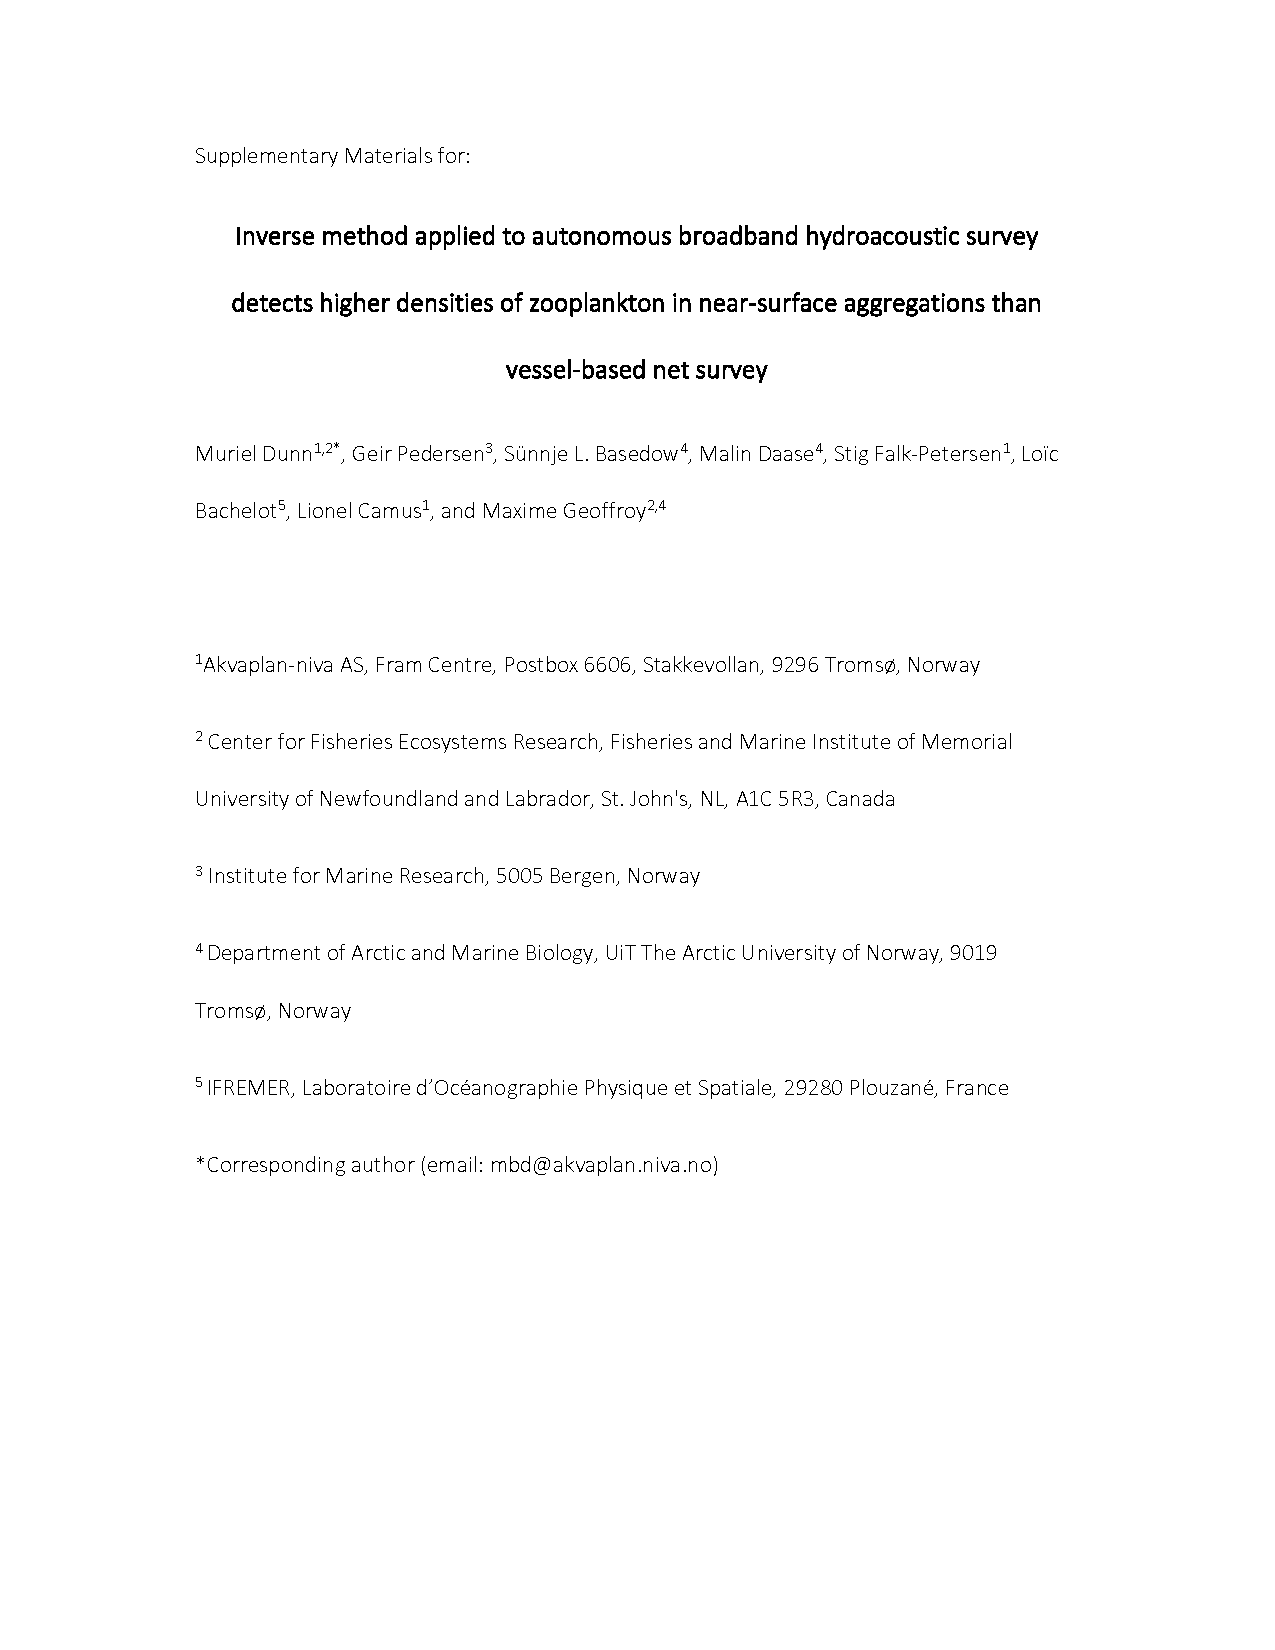
\includepdf[pages=-]{cjfas-2022-0105suppla.pdf}
\chapter{Ethics approval for AFKABAN experiments}
\label{apdx:Ethics1}


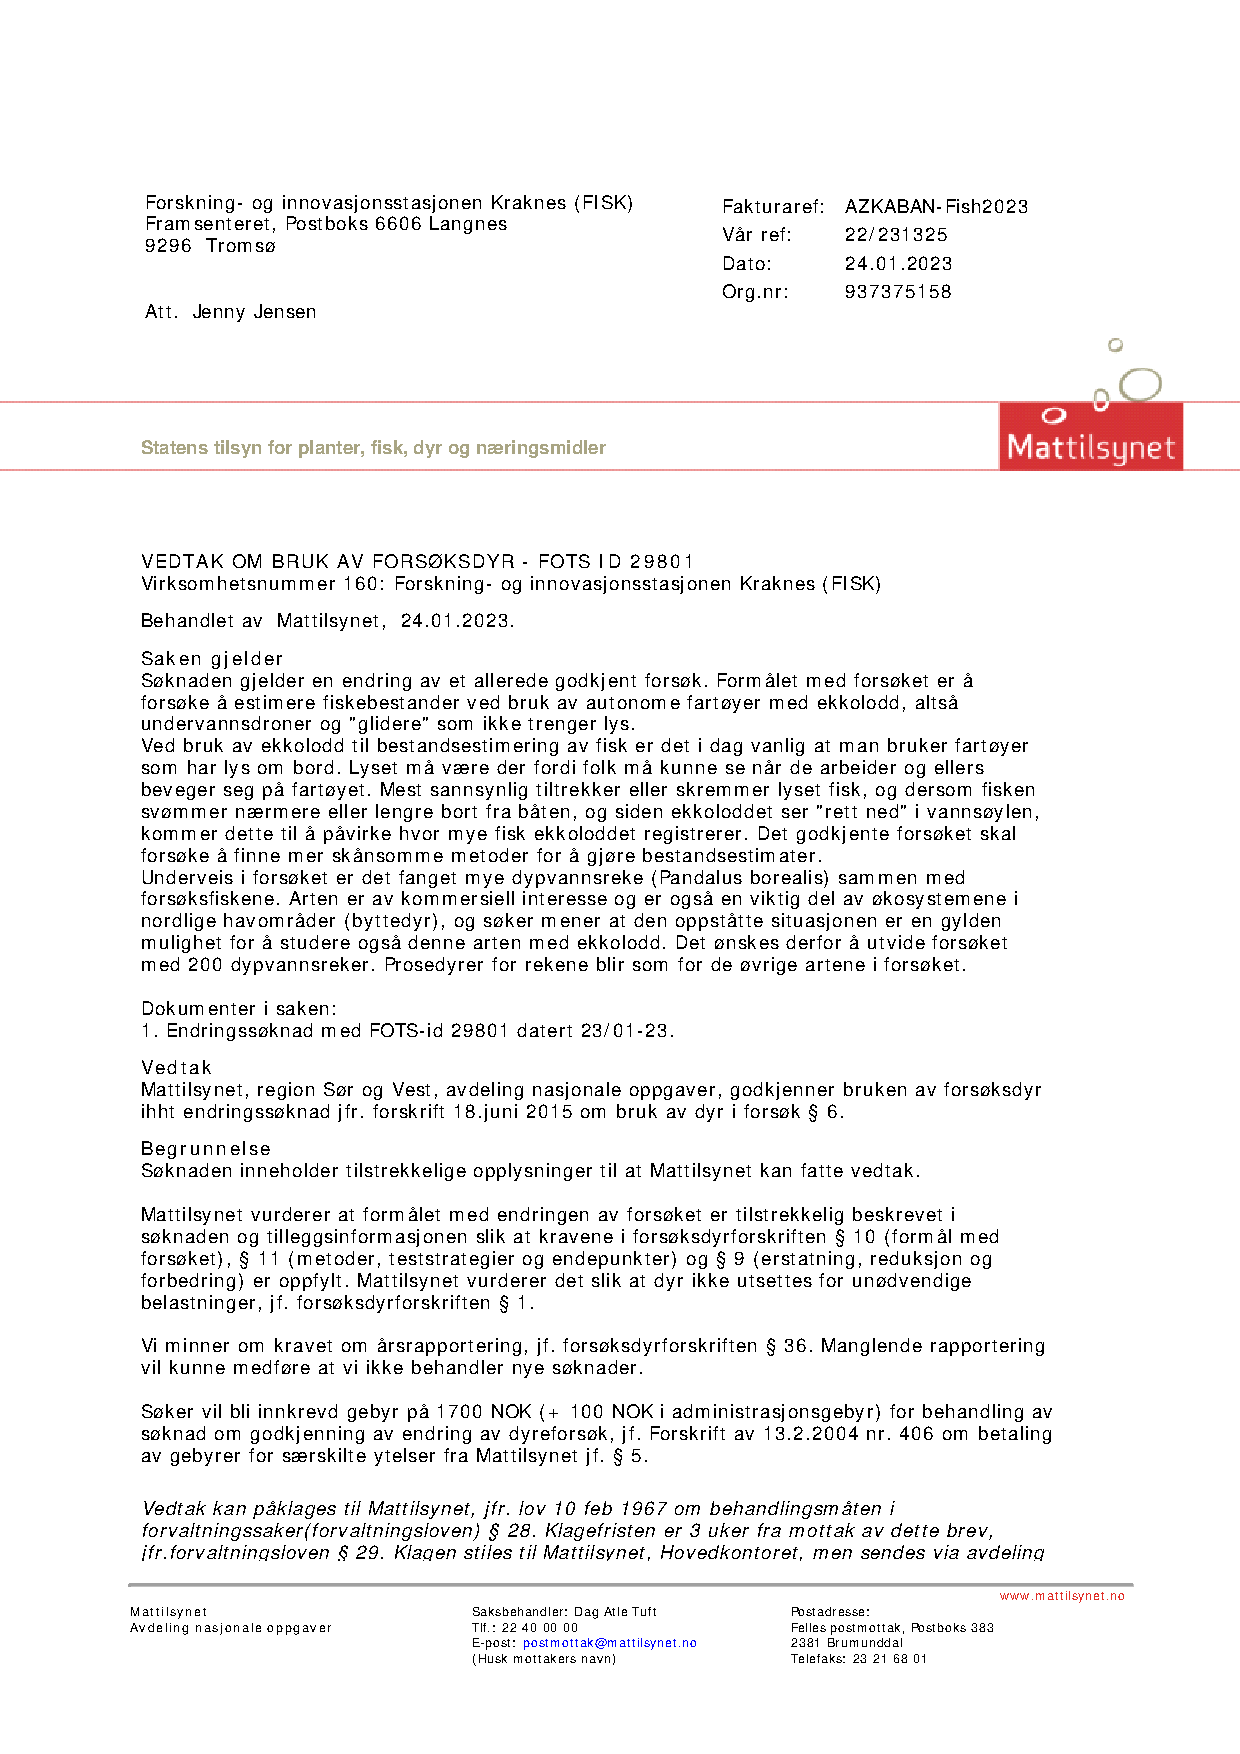
\includepdf[pages=-]{EthicsApproval}
\chapter{Supplementary Materials 2}
\label{apdx:SuppMat2}


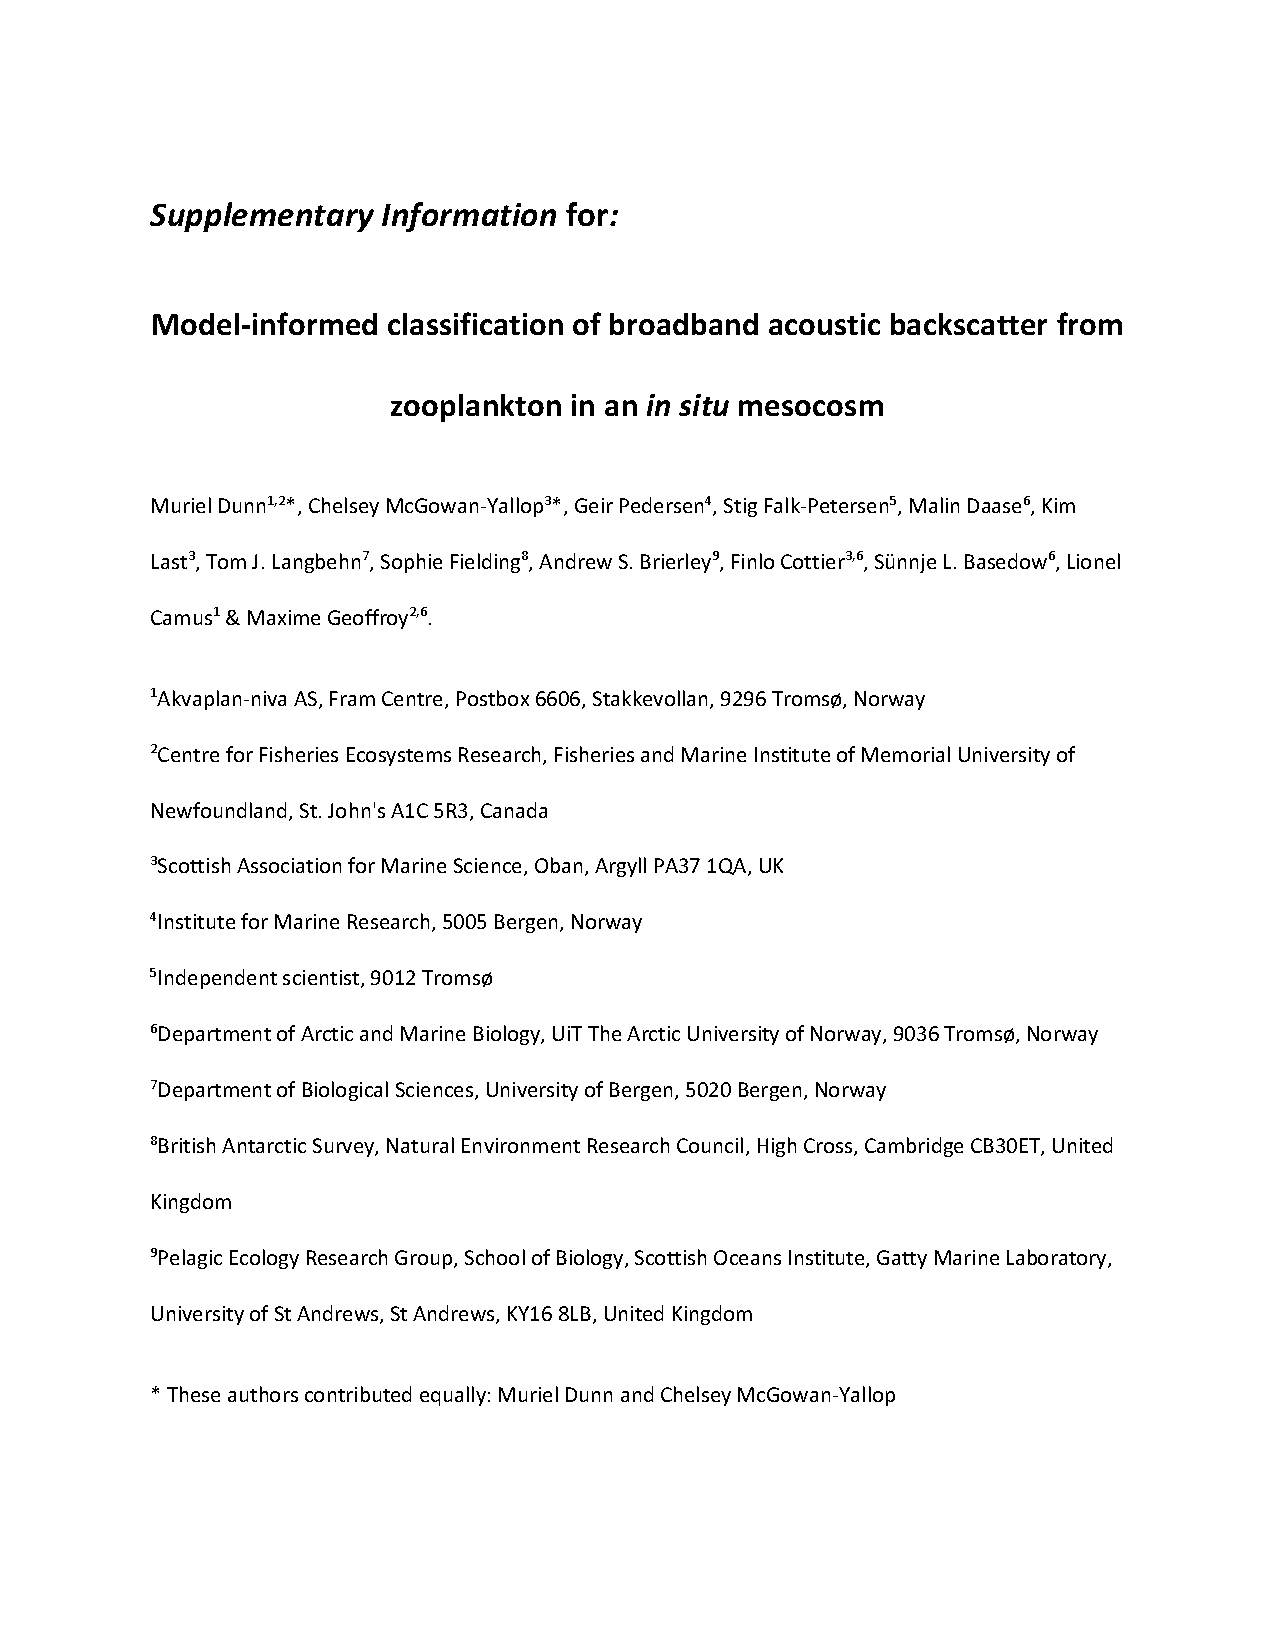
\includepdf[pages=-]{SupplementaryInformation_AZKABAN.pdf}
\chapter{Supplementary Materials 3}
\label{apdx:SuppMat3}


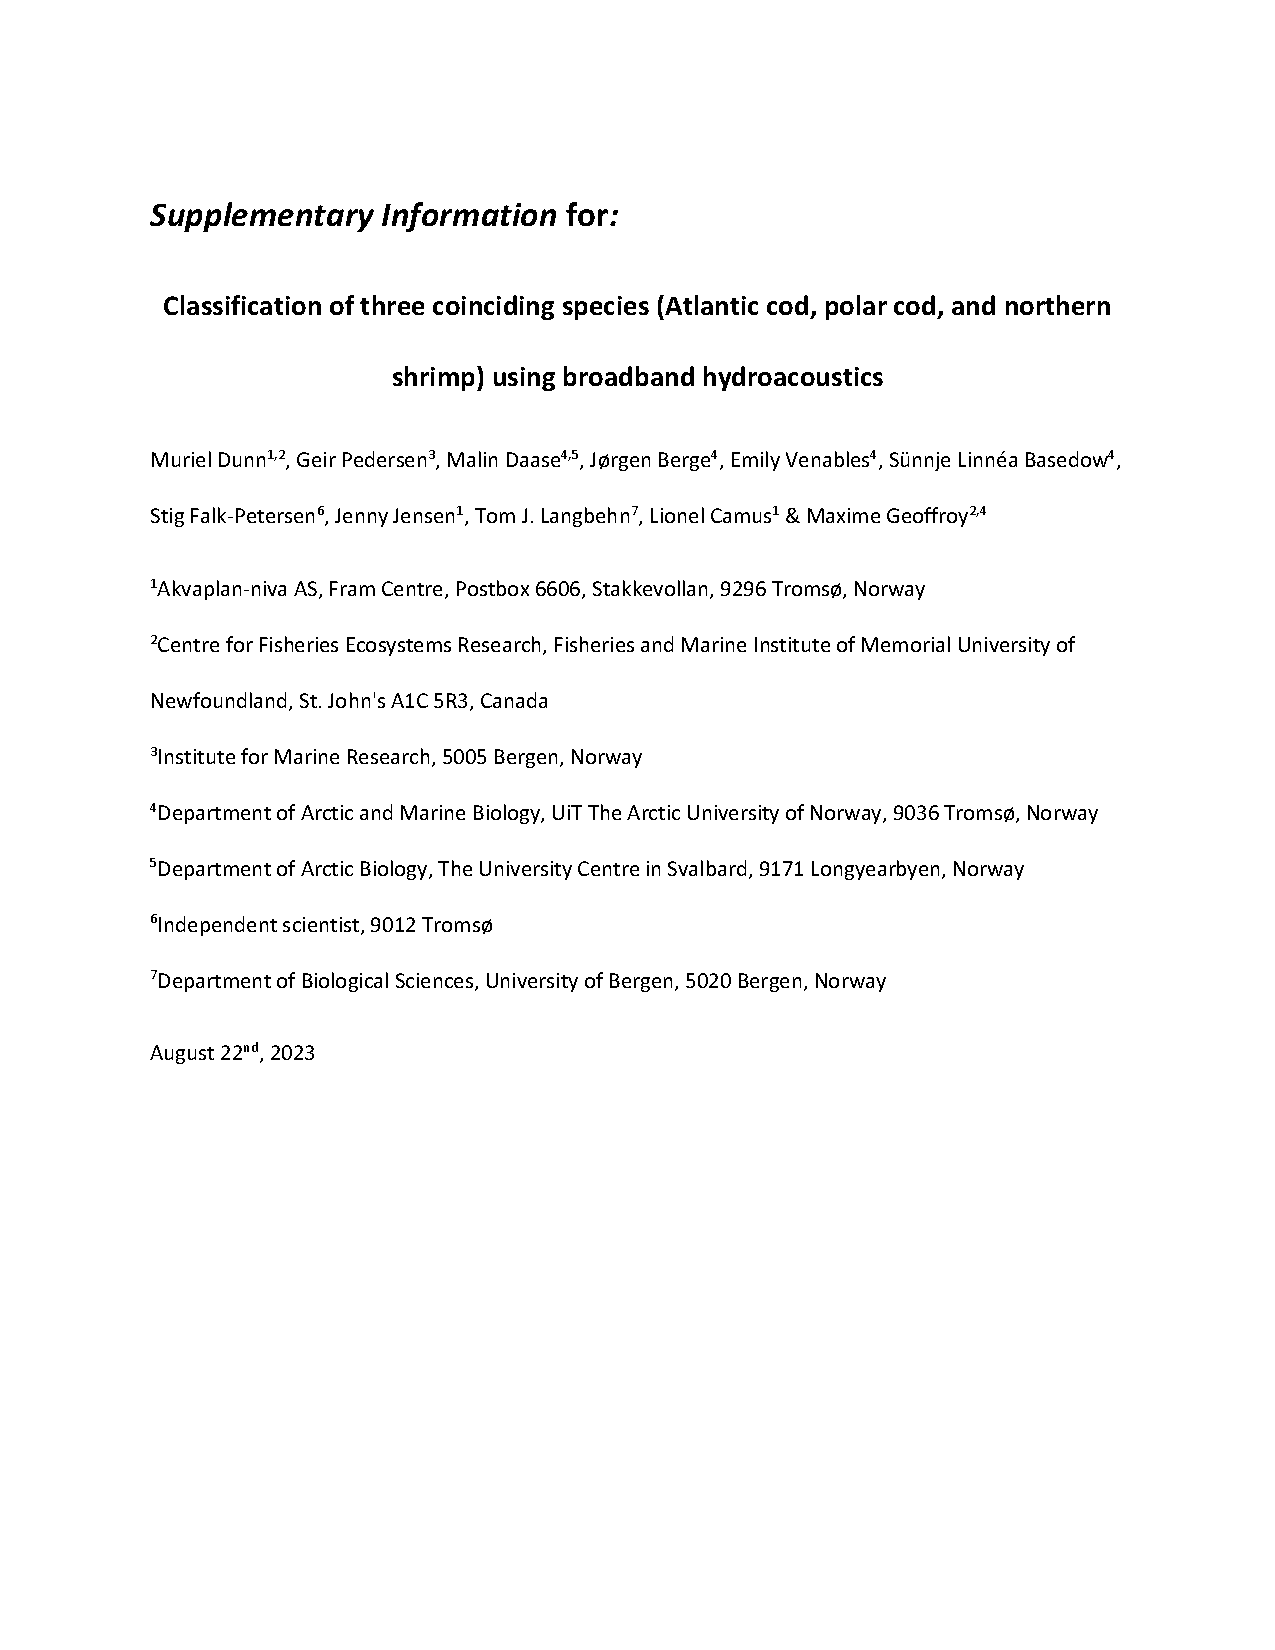
\includepdf[pages=-]{SupplementaryInformation_Classification.pdf}

\end{document}
